\documentclass[11pt,fleqn]{book} % Default font size and left-justified equations

%--------------------------------------------------------------------------
% Document geometry % Page margins
%--------------------------------------------------------------------------
\usepackage[margin=1in,headsep=10pt,a4paper]{geometry}

%--------------------------------------------------------------------------
% MinionPro fonts
%--------------------------------------------------------------------------
\IfFileExists{MinionPro.sty}{%
  \usepackage{MnSymbol}
  \usepackage{MinionPro}
  \usepackage{MyriadPro}
}{%
  \usepackage[T1]{fontenc}
  \usepackage{newtxtext}
  %\usepackage{eulervm}
  \usepackage{amssymb}%needed for \mathbb
}

%--------------------------------------------------------------------------
% Color scheme used in this book
%--------------------------------------------------------------------------
\usepackage{xcolor} % Required for specifying colors by name
\definecolor{ocre}{RGB}{243,102,25} % Define the orange color used for highlighting throughout the book
\definecolor{dkgreen}{rgb}{0,0.6,0}
\definecolor{delim}{RGB}{20,105,176}
\definecolor{background}{HTML}{EEEEEE}
\definecolor{Red}{rgb}{0.8666,0.03137,0.02352}
\definecolor{Blue}{rgb}{0.00784,0.67059,0.91764}
\definecolor{Darkgreen}{rgb}{0,0.68235,0}
\definecolor{Green}{rgb}{0,0.8,0}
\definecolor{Royalblue}{rgb}{0,0.2,0.91764}
\definecolor{Brickred}{rgb}{0.644541,0.164065,0.164065}
\definecolor{Brown}{rgb}{0.6,0.4,0.4}
\definecolor{Orange}{rgb}{1,0.647059,0}
\definecolor{Indigo}{rgb}{0.746105,0,0.996109}
\definecolor{Violet}{rgb}{0.308598,0.183597,0.308598}
\definecolor{Lightgrey}{rgb}{0.762951,0.762951,0.762951}
\definecolor{Darkgrey}{rgb}{0.503548,0.503548,0.503548}
\definecolor{Pink}{rgb}{1,0.6,0.6}
\definecolor{DarkBlue}{rgb}{0,0.08,0.45}
\definecolor{OliveDrab}{rgb}{0.41961,0.55686,0.13725}
\definecolor{LightMagenta}{cmyk}{0.1,0.8,0,0.1}
\definecolor{OliveD}{HTML}{6B8E23}
\definecolor{authorNoteColor}{rgb}{.8,0,0}
\newcommand{\Ochre}{\color{ocre}}
\newcommand{\Red}{\color{Brickred}}
\newcommand{\Blue}{\color{Royalblue}}
\newcommand{\Green}{\color{Darkgreen}}
\newcommand{\DarkGreen}{\color{Darkgreen}}
\newcommand{\Violet}{\color{Violet}}
\newcommand{\Indigo}{\color{Indigo}}
\newcommand{\Orange}{\color{Orange}}
\newcommand{\Brown}{\color{Brown}}
\newcommand{\OliveD}{\color{OliveD}}
\newcommand{\Pink}{\color{Pink}}


%--------------------------------------------------------------------------
% Bibliography : biblatex does not work with tufte-book
%--------------------------------------------------------------------------
\usepackage[style=numeric,
            citestyle=numeric-comp,
            sorting=none,
            sortcites=true,
            autopunct=true,
            babel=hyphen,
            hyperref=true,
            abbreviate=false,
            backref=true,
            backend=biber]{biblatex}
\addbibresource{../Bibliography.bib} % BibTeX bibliography file
\defbibheading{bibempty}{}

%--------------------------------------------------------------------------
% Graphics
%--------------------------------------------------------------------------
\usepackage[pdftex]{graphicx}
\DeclareGraphicsExtensions{{.png},{.pdf},{.jpg},{jpeg}}
\graphicspath{ {../figures/}}
\setkeys{Gin}{width=\linewidth,totalheight=\textheight,keepaspectratio}

%--------------------------------------------------------------------------
% Links
%--------------------------------------------------------------------------
\usepackage{hyperref}
\hypersetup{pdftex, colorlinks=true, linkcolor=blue, citecolor=blue, filecolor=blue, urlcolor=blue, pdftitle=, pdfauthor= , pdfsubject=, pdfkeywords=}

%--------------------------------------------------------------------------
% Code listing
%--------------------------------------------------------------------------
\usepackage{listings}

\lstset{ %
  basicstyle=\scriptsize\ttfamily,           % the size of the fonts that are used for the code
  backgroundcolor=\color{white},      % choose the background color. You must add \usepackage{color}
  showspaces=false,               % show spaces adding particular underscores
  showstringspaces=false,         % underline spaces within strings
  showtabs=false,                 % show tabs within strings adding particular underscores
  tabsize=2,                      % sets default tabsize to 2 spaces
  captionpos=b,                   % sets the caption-position to bottom
  breaklines=true,                % sets automatic line breaking
  breakatwhitespace=false,        % sets if automatic breaks should only happen at whitespace
  commentstyle=\color{dkgreen}\upshape,       % comment style
  escapeinside={\%*}{*)},            % if you want to add LaTeX within your code
  morekeywords={*,MPM,ICE,MPMICE}               % if you want to add more keywords to the set
}

\colorlet{punct}{red!60!black}
\colorlet{numb}{magenta!60!black}

\lstdefinelanguage{XML}
{
  morestring=[b]",
  morestring=[s]{>}{<},
  morecomment=[s]{<?}{?>},
  morestring=[s]{"}{"},
  morecomment=[s]{?}{?},
  morecomment=[s]{!--}{--},
  stringstyle=\color{black},
  identifierstyle=\color{DarkBlue},
  keywordstyle=\color{Brickred},
  backgroundcolor=\color{background},
  frame=lines,
  morekeywords={xmlns,version,type}% list your attributes here
}

\lstdefinelanguage{C++}
{
  keywordstyle=\color{Brickred},
  stringstyle=\color{red},
  identifierstyle=\color{DarkBlue},
  backgroundcolor=\color{background},
  frame=lines,
  morecomment=[l][\color{magenta}]{\#}
}

\lstdefinelanguage{Cpp}
{
  language=C++,
  commentstyle=\color{dkgreen}\upshape,   
  stringstyle=\color{red},
  identifierstyle=\color{DarkBlue},
  backgroundcolor=\color{background},
  frame=lines,
  deletekeywords={...},
  escapeinside={\%*}{*)},
  keywordstyle=\color{Brickred},
  morekeywords={ProblemSpecP, ProcessorGroup, SimulationController,%
                AMRSimulationController, RegridderCommon, SolverInterface,%
                SolverFactory, UintahParallelComponent, SimulationInterface,%
                ComponentFactory, LoadBalancerCommon, LoadBalancerFactory,%
                DataArchiver, Output, SchedulerCommon, SchedulerFactory,%
                ProblemSetupException, Exception,%
                Task, Level, Patch, Ghost, Example,%
                GridP, SimulationStateP, LevelP, SchedulerP,%
                PatchSubset, MaterialSubset, DataWarehouse,% 
                SFCXVariable, PerPatch, IntVector, NodeIterator,%
                VarLabel, MPMMaterial, PatchSet, ParticleSubset,%
                MPMFlags, FlowModel, ConstitutiveModel, MyModel, MyFlow, PlasticityState,%
                particleIndex, TangentModulusTensor, Matrix3, Vector,
                ElasticModuli, TabularPlasticity, ModelState_Tabular, ParticleVariable,
                constParticleVariable, delt_vartype, ElasticModuliModelFactory,%
                YieldConditionFactory, ElasticModuliModel, YieldCondition, CMData,
                ParticleLabelVariableMap, ParameterDict, TabularData, IndependentVar,
                DependentVar, IndexKey, json, DoubleVec1D, DoubleVec2D,
                int,char,double,float,unsigned, size_t,%
                string, istringstream, cerr, exit}, 
  morecomment=[l][\color{magenta}]{\#}
}


\lstdefinelanguage{JSON}{
    numbers=left,
    numberstyle=\scriptsize,
    stepnumber=1,
    numbersep=8pt,
    showstringspaces=false,
    breaklines=true,
    frame=lines,
    backgroundcolor=\color{background},
    literate=
     *{0}{{{\color{numb}0}}}{1}
      {1}{{{\color{numb}1}}}{1}
      {2}{{{\color{numb}2}}}{1}
      {3}{{{\color{numb}3}}}{1}
      {4}{{{\color{numb}4}}}{1}
      {5}{{{\color{numb}5}}}{1}
      {6}{{{\color{numb}6}}}{1}
      {7}{{{\color{numb}7}}}{1}
      {8}{{{\color{numb}8}}}{1}
      {9}{{{\color{numb}9}}}{1}
      {:}{{{\color{punct}{:}}}}{1}
      {,}{{{\color{punct}{,}}}}{1}
      {\{}{{{\color{delim}{\{}}}}{1}
      {\}}{{{\color{delim}{\}}}}}{1}
      {[}{{{\color{delim}{[}}}}{1}
      {]}{{{\color{delim}{]}}}}{1},
}


%--------------------------------------------------------------------------
% Colored boxes:  Must come after graphicx and verbatim
% and Tikz
%--------------------------------------------------------------------------
\RequirePackage{tikz}
\usetikzlibrary{shadings,shadows}
\usetikzlibrary{decorations.pathmorphing}
\usetikzlibrary{patterns}
\usetikzlibrary{intersections}
\usetikzlibrary{calc}

\usepackage{tcolorbox}
\tcbuselibrary{most}
\newtcolorbox{NoteBox}[1][]{%
  colback=yellow!50,
  colframe=yellow!20!black,
  before skip=2mm,after skip=3mm,
  boxrule=0.4pt,left=5mm,right=2mm,top=1mm,bottom=1mm,
  sharp corners,
  rounded corners=southeast,arc is angular,arc=3mm,
  underlay={%
    \path[fill=tcbcol@back!80!black] ([yshift=3mm]interior.south east)--++(-0.4,-0.1)--++(0.1,-0.2);
    \path[draw=tcbcol@frame,shorten <=-0.05mm,shorten >=-0.05mm] ([yshift=3mm]interior.south east)--++(-0.4,-0.1)--++(0.1,-0.2);
    \path[fill=yellow!50!black,draw=none] (interior.south west) rectangle node[white]{\Huge\bfseries !} ([xshift=4mm]interior.north west);
    },
  drop fuzzy shadow,%
  #1}

\newtcolorbox{WarningBox}[1][]{%
  colback=pink!50,
  colframe=pink!20!black,
  before skip=2mm,after skip=3mm,
  boxrule=0.4pt,left=5mm,right=2mm,top=1mm,bottom=1mm,
  sharp corners,
  rounded corners=southeast,arc is angular,arc=3mm,
  underlay={%
    \path[fill=tcbcol@back!80!black] ([yshift=3mm]interior.south east)--++(-0.4,-0.1)--++(0.1,-0.2);
    \path[draw=tcbcol@frame,shorten <=-0.05mm,shorten >=-0.05mm] ([yshift=3mm]interior.south east)--++(-0.4,-0.1)--++(0.1,-0.2);
    \path[fill=pink!50!black,draw=none] (interior.south west) rectangle node[white]{\Huge\bfseries !} ([xshift=4mm]interior.north west);
    },
  drop fuzzy shadow,%
  #1}

\tcbuselibrary{skins}
\newtcolorbox[auto counter,number within=chapter]{ExampleBox}[1][]{%
  enhanced,
  colback=white,
  colframe=green!65!black,
  enlarge top by=10mm,
  overlay={%
    \path[fill=blue!65,line width=.4mm] (frame.north west)--++(17mm,0)coordinate(n2)--++(0,8mm)--++(-20mm,0) arc (-90:90:-4mm)--cycle;
    \node at ([shift={(5mm,4mm)}]frame.north west){\color{white}{\textbf{\sffamily EXAMPLE}}};
    \path[fill=green!65!blue] ([xshift=.4mm]n2)--++(0,8mm)--++(7mm,0)--++(0,-8mm)--cycle;
    \node at ([shift={(4mm,4mm)}]n2){\color{white}{\textbf{\sffamily \thetcbcounter}}};
    %\node at ([shift={(18mm,4mm)}]n2){\itshape\textbf{\sffamily Solution}};
  },
  #1}

\usetikzlibrary{calc}
\usetikzlibrary{positioning}
\tcbuselibrary{skins}
\newtcolorbox[auto counter,number within=section]{SummaryBox}[2][]{%
  enhanced,
  colback=white,
  colframe=ocre,
  enlarge top by=10mm,
  overlay={%
    \path[fill=ocre!65,line width=.4mm] (frame.north west)--++(17mm,0)coordinate(n2)--++(0,8mm)--++(-20mm,0) arc (-90:90:-4mm)--cycle;
    \node at ([shift={(5mm,4mm)}]frame.north west){\color{white}{\textbf{\sffamily Summary}}};
    \path[fill=ocre] ([xshift=.4mm]n2)--++(0,8mm)--++(10mm,0)--++(0,-8mm)--cycle;
    \node (A) at ([shift={(5mm,4mm)}]n2){\color{white}{\textbf{\sffamily \thetcbcounter}}};
    \node [right=0.5cm of A] {\itshape\textbf{\sffamily #2}};
  },
  #1}


%--------------------------------------------------------------------------
% Structure of the document
%--------------------------------------------------------------------------
%%----------------------------------------------------------------------------------------
%	VARIOUS REQUIRED PACKAGES
%----------------------------------------------------------------------------------------

\usepackage{titlesec} % Allows customization of titles

%\usepackage{graphicx} % Required for including pictures
%\graphicspath{{./Pictures/}} % Specifies the directory where pictures are stored

\usepackage{lipsum} % Inserts dummy text

\usepackage{tikz} % Required for drawing custom shapes

\usepackage[english]{babel} % English language/hyphenation

\usepackage{enumitem} % Customize lists
\setlist{nolistsep} % Reduce spacing between bullet points and numbered lists

\usepackage{booktabs} % Required for nicer horizontal rules in tables

\usepackage{eso-pic} % Required for specifying an image background in the title page

%----------------------------------------------------------------------------------------
%	MAIN TABLE OF CONTENTS
%----------------------------------------------------------------------------------------

\usepackage{titletoc} % Required for manipulating the table of contents

\contentsmargin{0cm} % Removes the default margin

% Chapter text styling
\titlecontents{chapter}[1.25cm] % Indentation
{\addvspace{15pt}\large\sffamily\bfseries} % Spacing and font options for chapters
{\color{ocre!60}\contentslabel[\Large\thecontentslabel]{1.25cm}\color{ocre}} % Chapter number
{}  
{\color{ocre!60}\normalsize\sffamily\bfseries\;\titlerule*[.5pc]{.}\;\thecontentspage} % Page number

% Section text styling
\titlecontents{section}[1.55cm] % Indentation
{\addvspace{5pt}\sffamily} % Spacing and font options for sections
{\contentslabel[\thecontentslabel]{1.25cm}} % Section number
{}
{\sffamily\hfill\color{black}\thecontentspage} % Page number
[]

% Subsection text styling
\titlecontents{subsection}[1.85cm] % Indentation
{\addvspace{1pt}\sffamily\small} % Spacing and font options for subsections
{\contentslabel[\thecontentslabel]{1.25cm}} % Subsection number
{}
{\sffamily\;\titlerule*[.5pc]{.}\;\thecontentspage} % Page number
[] 

%----------------------------------------------------------------------------------------
%	MINI TABLE OF CONTENTS IN CHAPTER HEADS
%----------------------------------------------------------------------------------------

% Section text styling
\titlecontents{lsection}[0em] % Indendating
{\footnotesize\sffamily} % Font settings
{}
{}
{}

% Subsection text styling
\titlecontents{lsubsection}[.5em] % Indentation
{\normalfont\footnotesize\sffamily} % Font settings
{}
{}
{}
 
%----------------------------------------------------------------------------------------
%	PAGE HEADERS
%----------------------------------------------------------------------------------------

\usepackage{fancyhdr} % Required for header and footer configuration

\pagestyle{fancy}
\renewcommand{\chaptermark}[1]{\markboth{\sffamily\normalsize\bfseries #1}{}} % Chapter text font settings
\renewcommand{\sectionmark}[1]{\markright{\sffamily\normalsize\thesection\hspace{5pt}#1}{}} % Section text font settings
\fancyhf{} \fancyhead[LE,RO]{\sffamily\normalsize\thepage} % Font setting for the page number in the header
\fancyhead[LO]{\rightmark} % Print the nearest section name on the left side of odd pages
\fancyhead[RE]{\leftmark} % Print the current chapter name on the right side of even pages
\renewcommand{\headrulewidth}{0.5pt} % Width of the rule under the header
\addtolength{\headheight}{2.5pt} % Increase the spacing around the header slightly
\renewcommand{\footrulewidth}{0pt} % Removes the rule in the footer
\fancypagestyle{plain}{\fancyhead{}\renewcommand{\headrulewidth}{0pt}} % Style for when a plain pagestyle is specified

% Removes the header from odd empty pages at the end of chapters
\makeatletter
\renewcommand{\cleardoublepage}{
\clearpage\ifodd\c@page\else
\hbox{}
\vspace*{\fill}
\thispagestyle{empty}
\newpage
\fi}

%----------------------------------------------------------------------------------------
%	THEOREM STYLES
%----------------------------------------------------------------------------------------

\usepackage{amsmath} % For including math equations, theorems, symbols, etc
\usepackage{amsfonts} % For including math equations, theorems, symbols, etc
%\usepackage{amssymb} % For including math equations, theorems, symbols, etc
\usepackage{amsthm} % For including math equations, theorems, symbols, etc

\newcommand{\intoo}[2]{\mathopen{]}#1\,;#2\mathclose{[}}
\newcommand{\ud}{\mathop{\mathrm{{}d}}\mathopen{}}
\newcommand{\intff}[2]{\mathopen{[}#1\,;#2\mathclose{]}}
\newtheorem{notation}{Notation}[chapter]

\newtheoremstyle{ocrenum} % Theorem style name
{7pt} % Space above
{7pt} % Space below
{\normalfont} % Body font
{} % Indent amount
{\small\bf\sffamily\color{ocre}} % Theorem head font
{\;\;} % Punctuation after theorem head
{0.25em} % Space after theorem head
{\small\sffamily\color{ocre}\thmname{#1}\thmnumber{\@ifnotempty{#1}{ }\@upn{#2}} % Theorem text (e.g. Theorem 2.1)
\thmnote{\ {\the\thm@notefont\sffamily\bfseries\color{black}--- #3.}}} % Optional theorem note
\renewcommand{\qedsymbol}{$\blacksquare$} % Optional qed square

\newtheoremstyle{blacknumex} % Theorem style name
{7pt} % Space above
{7pt} % Space below
{\normalfont} % Body font
{} % Indent amount
{\small\bf\sffamily} % Theorem head font
{\;\;} % Punctuation after theorem head
{0.25em} % Space after theorem head
{\small\sffamily{\tiny\ensuremath{\blacksquare}}\ \thmname{#1}\thmnumber{\@ifnotempty{#1}{ }\@upn{#2}} % Theorem text (e.g. Theorem 2.1)
\thmnote{\ {\the\thm@notefont\sffamily\bfseries--- #3.}}} % Optional theorem note

\newtheoremstyle{blacknum} % Theorem style name
{7pt} % Space above
{7pt} % Space below
{\normalfont} % Body font
{} % Indent amount
{\small\bf\sffamily} % Theorem head font
{\;\;} % Punctuation after theorem head
{0.25em} % Space after theorem head
{\small\sffamily\thmname{#1}\thmnumber{\@ifnotempty{#1}{ }\@upn{#2}} % Theorem text (e.g. Theorem 2.1)
\thmnote{\ {\the\thm@notefont\sffamily\bfseries--- #3.}}} % Optional theorem note
\makeatother

% Defines the theorem text style for each type of theorem to one of the three styles above
\theoremstyle{ocrenum}
\newtheorem{theoremeT}{Theorem}[chapter]
\newtheorem{proposition}{Proposition}[chapter]
\newtheorem{problem}{Problem}[chapter]
\newtheorem{exerciseT}{Exercise}[chapter]
\theoremstyle{blacknumex}
\newtheorem{exampleT}{Example}[chapter]
\theoremstyle{blacknum}
\newtheorem{vocabulary}{Vocabulary}[chapter]
\newtheorem{definitionT}{Definition}[chapter]
\newtheorem{corollaryT}{Corollary}[chapter]

%----------------------------------------------------------------------------------------
%	DEFINITION OF COLORED BOXES
%----------------------------------------------------------------------------------------

\RequirePackage[framemethod=default]{mdframed} % Required for creating the theorem, definition, exercise and corollary boxes

% Theorem box
\newmdenv[skipabove=7pt,
skipbelow=7pt,
backgroundcolor=black!5,
linecolor=ocre,
innerleftmargin=5pt,
innerrightmargin=5pt,
innertopmargin=5pt,
leftmargin=0cm,
rightmargin=0cm,
innerbottommargin=5pt]{tBox}

% Exercise box	  
\newmdenv[skipabove=7pt,
skipbelow=7pt,
rightline=false,
leftline=true,
topline=false,
bottomline=false,
backgroundcolor=ocre!10,
linecolor=ocre,
innerleftmargin=5pt,
innerrightmargin=5pt,
innertopmargin=5pt,
innerbottommargin=5pt,
leftmargin=0cm,
rightmargin=0cm,
linewidth=4pt]{eBox}	

% Definition box
\newmdenv[skipabove=10pt,
skipbelow=10pt,
rightline=false,
leftline=true,
topline=false,
bottomline=false,
linecolor=ocre,
innerleftmargin=5pt,
innerrightmargin=5pt,
innertopmargin=0pt,
leftmargin=0cm,
rightmargin=0cm,
linewidth=4pt,
innerbottommargin=0pt]{dBox}	

% Corollary box
\newmdenv[skipabove=7pt,
skipbelow=7pt,
rightline=false,
leftline=true,
topline=false,
bottomline=false,
linecolor=gray,
backgroundcolor=black!5,
innerleftmargin=5pt,
innerrightmargin=5pt,
innertopmargin=5pt,
leftmargin=0cm,
rightmargin=0cm,
linewidth=4pt,
innerbottommargin=5pt]{cBox}				  
		  

% Creates an environment for each type of theorem and assigns it a theorem text style from the "Theorem Styles" section above and a colored box from above
\newenvironment{theorem}{\begin{tBox}\begin{theoremeT}}{\end{theoremeT}\end{tBox}}
\newenvironment{exercise}{\begin{eBox}\begin{exerciseT}}{\hfill{\color{ocre}\tiny\ensuremath{\blacksquare}}\end{exerciseT}\end{eBox}}				  
\newenvironment{definition}{\begin{dBox}\begin{definitionT}}{\end{definitionT}\end{dBox}}	
\newenvironment{example}{\begin{exampleT}}{\hfill{\tiny\ensuremath{\blacksquare}}\end{exampleT}}		
\newenvironment{corollary}{\begin{cBox}\begin{corollaryT}}{\end{corollaryT}\end{cBox}}	

%----------------------------------------------------------------------------------------
%	REMARK ENVIRONMENT
%----------------------------------------------------------------------------------------

\newenvironment{remark}{\par\vskip10pt\small % Vertical white space above the remark and smaller font size
\begin{list}{}{
\leftmargin=35pt % Indentation on the left
\rightmargin=25pt}\item\ignorespaces % Indentation on the right
\makebox[-2.5pt]{\begin{tikzpicture}[overlay]
\node[draw=ocre!60,line width=1pt,circle,fill=ocre!25,font=\sffamily\bfseries,inner sep=2pt,outer sep=0pt] at (-15pt,0pt){\textcolor{ocre}{R}};\end{tikzpicture}} % Orange R in a circle
\advance\baselineskip -1pt}{\end{list}\vskip5pt} % Tighter line spacing and white space after remark

%----------------------------------------------------------------------------------------
%	SECTION NUMBERING IN THE MARGIN
%----------------------------------------------------------------------------------------

\makeatletter
\renewcommand{\@seccntformat}[1]{\llap{\textcolor{ocre}{\csname the#1\endcsname}\hspace{1em}}}                    
\renewcommand{\section}{\@startsection{section}{1}{\z@}
{-4ex \@plus -1ex \@minus -.4ex}
{1ex \@plus.2ex }
{\normalfont\large\sffamily\bfseries}}
\renewcommand{\subsection}{\@startsection {subsection}{2}{\z@}
{-3ex \@plus -0.1ex \@minus -.4ex}
{0.5ex \@plus.2ex }
{\normalfont\sffamily\bfseries}}
\renewcommand{\subsubsection}{\@startsection {subsubsection}{3}{\z@}
{-2ex \@plus -0.1ex \@minus -.2ex}
{0.2ex \@plus.2ex }
{\color{teal}\normalfont\small\sffamily\bfseries}}                        
\renewcommand\paragraph{\@startsection{paragraph}{4}{\z@}
{-2ex \@plus-.2ex \@minus .2ex}
{0.1ex}
{\normalfont\small\sffamily\bfseries}}

%----------------------------------------------------------------------------------------
%	CHAPTER HEADINGS
%----------------------------------------------------------------------------------------

\newcommand{\thechapterimage}{}
\newcommand{\chapterimage}[1]{\renewcommand{\thechapterimage}{#1}}
\def\thechapter{\arabic{chapter}}
\def\@makechapterhead#1{
\thispagestyle{empty}
{\centering \normalfont\sffamily
\ifnum \c@secnumdepth >\m@ne
\if@mainmatter
\startcontents
\begin{tikzpicture}[remember picture,overlay]
\node at (current page.north west)
{\begin{tikzpicture}[remember picture,overlay]

\node[anchor=north west,inner sep=0pt] at (14,-0.5) {\includegraphics[width=0.3\paperwidth]{\thechapterimage}};

%Commenting the 3 lines below removes the small contents box in the chapter heading
%\draw[fill=white,opacity=.6] (1cm,0) rectangle (8cm,-7cm);
%\node[anchor=north west] at (1cm,.25cm) {\parbox[t][8cm][t]{6.5cm}{\huge\bfseries\flushleft \printcontents{l}{1}{\setcounter{tocdepth}{2}}}};

\draw[anchor=west] (5cm,-8cm) node [rounded corners=25pt,fill=white,fill opacity=1.0,text opacity=1,draw=ocre,draw opacity=1,line width=2pt,inner sep=15pt]{\huge\sffamily\bfseries\textcolor{black}{\thechapter\ ---\ #1\vphantom{plPQq}\makebox[22cm]{}}};
\end{tikzpicture}};
\end{tikzpicture}}\par\vspace*{200\p@}
\fi
\fi
}
\def\@makeschapterhead#1{
\thispagestyle{empty}
{\centering \normalfont\sffamily
\ifnum \c@secnumdepth >\m@ne
\if@mainmatter
\startcontents
\begin{tikzpicture}[remember picture,overlay]
\node at (current page.north west)
{\begin{tikzpicture}[remember picture,overlay]
\node[anchor=north west] at (14,-0.5) {\includegraphics[width=0.3\paperwidth]{\thechapterimage}};
\draw[anchor=west] (5cm,-8cm) node [rounded corners=25pt,fill=white,opacity=.7,inner sep=15.5pt]{\huge\sffamily\bfseries\textcolor{black}{\vphantom{plPQq}\makebox[22cm]{}}};
\draw[anchor=west] (5cm,-8cm) node [rounded corners=25pt,draw=ocre,line width=2pt,inner sep=15pt]{\huge\sffamily\bfseries\textcolor{black}{#1\vphantom{plPQq}\makebox[22cm]{}}};
\end{tikzpicture}};
\end{tikzpicture}}\par\vspace*{200\p@}
\fi
\fi
}
\makeatother


%--------------------------------------------------------------------------
% Other packges
%--------------------------------------------------------------------------
%\usepackage{bm}%to get bold math symbols
%\usepackage[pdftex]{graphicx}
%\usepackage{verbatim}
%\usepackage[tt]{titlepic}%package i downloaded to put a pic in the titlepage
%\usepackage{helvet}
%\usepackage[usenames,dvipsnames]{xcolor}%options to use names like redviolet and others
%\usepackage{xspace}
%\usepackage[mathscr]{eucal}%Defines which font to use with \mathscr
%\usepackage{enumerate}
%\usepackage{comment}
%\usepackage{mathrsfs}
%\usepackage{floatrow}%automatically centers graphics without needing a \center command on each and every figure.

% Index
%\usepackage{calc} % For simpler calculation - used for spacing the index letter headings correctly
%\usepackage{makeidx} % Required to make an index

%-------------------------------------------------------
% For appendix
%-------------------------------------------------------
%\usepackage{esint}
\usepackage[toc,page,title,titletoc]{appendix}

%\usepackage{makeidx} % Used to generate the index

%\usepackage{xspace} % Used for printing a trailing space better than using a tilde (~) using the \xspace command

%\usepackage{epsf}
%\usepackage{epsfig}
%\usepackage{boxedminipage}
%\usepackage{stmaryrd}
%\usepackage{cancel}

%-------------------------------------------------------
% For text wrap around figures and captions for subfigures
%-------------------------------------------------------
\usepackage{wrapfig}
\usepackage{subcaption}

%-------------------------------------------------------
% For underlines
%-------------------------------------------------------
\usepackage[normalem]{ulem}

%-------------------------------------------------------
% For parallel columns
%-------------------------------------------------------
\usepackage{paracol}

%-------------------------------------------------------
% For algorithms
%-------------------------------------------------------
\usepackage{algorithm, algpseudocode, float}
%\usepackage{algorithmic}

\makeatletter
\newenvironment{breakablealgorithm}
  {% \begin{breakablealgorithm}
   \begin{center}
     \refstepcounter{algorithm}% New algorithm
     \hrule height.8pt depth0pt \kern2pt% \@fs@pre for \@fs@ruled
     \renewcommand{\caption}[2][\relax]{% Make a new \caption
       {\raggedright\textbf{\ALG@name~\thealgorithm} ##2\par}%
       \ifx\relax##1\relax % #1 is \relax
         \addcontentsline{loa}{algorithm}{\protect\numberline{\thealgorithm}##2}%
       \else % #1 is not \relax
         \addcontentsline{loa}{algorithm}{\protect\numberline{\thealgorithm}##1}%
       \fi
       \kern2pt\hrule\kern2pt
     }
  }{% \end{breakablealgorithm}
     \kern2pt\hrule\relax% \@fs@post for \@fs@ruled
   \end{center}
  }
\makeatother
\renewcommand{\algorithmiccomment}[1]{\hfill{\color{ocre}$\triangleright$\textit{#1}}}



%\newcommand{\AuthorNote}[1]{{\color{authorNoteColor} \sffamily{\textbf{#1}}}}

\newcommand{\Vaango}{\textsc{Vaango}\,}
\newcommand{\Uintah}{\textsc{Uintah}\,}
\newcommand{\MPM}{\textsc{MPM}\,}
\newcommand{\ICE}{\textsc{ICE}\,}
\newcommand{\MPMICE}{\textsc{MPMICE}\,}
\newcommand{\Arena}{\textsc{Arena}\,}
\newcommand{\Visit}{\textsc{VisIt}\,}
\newcommand{\Parsim}{\textsc{ParSim}\,}
\newcommand{\Textsfc}[1]{{\OliveD \textsf{#1}}\,}
\newcommand{\Textbfc}[1]{{\Pink \textsf{#1}}\,}
\newcommand{\Textttc}[1]{{\DarkGreen \texttt{#1}}\,}

%Wide bar
\newcommand{\overbar}[1]{\mkern 1.5mu\overline{\mkern-1.5mu#1\mkern-1.5mu}\mkern 1.5mu}
\renewcommand{\bar}[1]{\overbar{#1}}
\renewcommand{\widehat}[1]{\hat{#1}}

%__________________________________
% new commands for all sections
\newcommand{\BBComment}[1]{ \marginpar{{\scriptsize \color{red} #1 }}}
\newcommand{\red}[1]{\color{red} {#1} \color{black}}
\newcommand{\TT}[1]{\ensuremath{\tt{#1}\normalfont}}

% MPM & ICE
\newcommand{\tn}[1]{\mbox{\ensuremath{\mathbf{#1}}}}
\newcommand{\sig}{\mbox{\boldmath $\sigma \!\!$ \unboldmath}}
\newcommand{\bnabla} {\mbox {\boldmath $\nabla \!\!$ \unboldmath}}
\newcommand{\taubold} {\mbox{\boldmath $\tau \!\!$ \unboldmath}}
\newcommand{\f}{\ensuremath{f^{\theta}_r} }

\newcommand{\Texp}{\rm{exp}}
\newcommand{\Delt}{\ensuremath{\Delta t}}
\newcommand{\Epj}{\ensuremath{\epsilon_{p,j}}}
\newcommand{\Epo}{\ensuremath{\epsilon_{p,0}}}
\newcommand{\lambdadot}{\ensuremath{\dot{\lambda}}}
\def\bfE{{\bf E}}

\newcommand{\hangp}[1]{\makebox[0pt][r]{(}#1\makebox[0pt][l]{)}} % New command to create parentheses around text in tables which take up no horizontal space - this improves column spacing
\newcommand{\hangstar}{\makebox[0pt][l]{*}} % New command to create asterisks in tables which take up no horizontal space - this improves column spacing

\newcommand{\monthyear}{\ifcase\month\or January\or February\or March\or April\or May\or June\or July\or August\or September\or October\or November\or December\fi\space\number\year} % A command to print the current month and year

\newcommand{\blankpage}{\newpage\hbox{}\thispagestyle{empty}\newpage} % Command to insert a blank page

\def\rmd{{\rm d}}
\def\rme{{\rm e}}
\def\rmf{{\rm f}}
\def\rmr{{\rm r}}
\def\rmR{{\rm R}}
\def\rms{{\rm s}}
\def\bfd{{\bf d}}
\def\bfE{{\bf E}}
\def\bfF{{\bf F}}
\def\bff{{\bf f}}
\def\bfg{{\bf g}}
\def\bfI{{\bf I}}
\def\bfj{{\bf j}}
\def\bfm{{\bf m}}
\def\bfr{{\bf r}}
\def\bfx{{\bf x}}
\def\bfu{{\bf u}}
\def\rmg{{\rm g}}
\def\bfa{{\bf a}}
\def\bfG{{\bf G}}
\def\bfv{{\bf v}}
\def\tdot{{\textstyle\cdot}}

\pdfcompresslevel=9
%\raggedright

\newcommand{\handout}[3]{
        \begin{center}
         % \copyright 
          Biswajit Banerjee \hspace{4.2in} University of Utah\\
          \vspace{10pt}
          {\Large\bf Waves in Composites and Metamaterials}\\
          \vspace{6pt}
          (Instructor: Prof. G. W. Milton)
        \end{center}
        \vspace{8pt}\noindent
        %\begin{center}
        {\underline{\makebox[7.0in]{\large\bf\noindent
                \makebox[1.5in][l]{#1~~~} \hfill {~~~#2~~~} \hfill
                \makebox[1.5in][r]{~~~#3}}}}
        %\end{center}
        }

\newcommand{\heading}[1]{
        \begin{center}{\large\bf{#1}}\end{center}}

\newcommand{\subheading}[1]{
        \begin{center}{\normalsize\bf{#1}}\end{center}}

\newcommand{\subsubheading}[1]{
        \begin{center}{\small\bf{#1}}\end{center}}

\newcommand{\Heading}[1]{
        \vspace{12pt}\begin{center}{\Large\bf{#1}}\end{center}}

\newcommand{\Subheading}[1]{
        \vspace{8pt}\begin{center}{\large\bf{#1}}\end{center}}

\newcommand{\Jump}[1]{\ensuremath{\llbracket#1\rrbracket}}
\newcommand{\Blimitx}[1]{\ensuremath{\left[#1\right]_{x_a}^{x_b}}}
\newcommand{\Deriv}[2]{\ensuremath{\cfrac{d#1}{d#2}}}
\newcommand{\MDeriv}[2]{\ensuremath{\cfrac{D#1}{D#2}}}
\newcommand{\DDeriv}[2]{\ensuremath{\cfrac{d^2#1}{d#2^2}}}
\newcommand{\DDDeriv}[2]{\ensuremath{\cfrac{d^3#1}{d#2^3}}}
\newcommand{\DDDDeriv}[2]{\ensuremath{\cfrac{d^4#1}{d#2^4}}}
\newcommand{\Intx}{\ensuremath{\int_{x_a}^{x_b}}}
\newcommand{\IntX}{\ensuremath{\int_{X_a}^{X_b}}}
\newcommand{\Intiso}{\ensuremath{\int_{-1}^{1}}}
\newcommand{\IntOmegaA}{\ensuremath{\int_{\Omega_0}}}
\newcommand{\IntOmega}{\ensuremath{\int_{\Omega}}}
\newcommand{\IntDOmega}{\ensuremath{\int_{\partial\Omega}}}
\newcommand{\Norm}[2]{\ensuremath{\left\lVert#1\right\rVert_{#2}}}
\newcommand{\norm}[1]{\ensuremath{\left\lVert#1\right\rVert}}
\newcommand{\Var}[1]{\ensuremath{\delta #1}}
\newcommand{\DelT}{\ensuremath{\Delta t}}
\newcommand{\CalA}{\ensuremath{\mathcal{A}}}
\newcommand{\CalB}{\ensuremath{\mathcal{B}}}
\newcommand{\CalC}{\ensuremath{\mathcal{C}}}
\newcommand{\CalF}{\ensuremath{\mathcal{F}}}
\newcommand{\CalL}{\ensuremath{\mathcal{L}}}
\newcommand{\CalM}{\ensuremath{\mathcal{M}}}
\newcommand{\BCalM}{\ensuremath{\boldsymbol{\CalM}}}
\newcommand{\CalN}{\ensuremath{\mathcal{N}}}
\newcommand{\CalP}{\ensuremath{\mathcal{P}}}
\newcommand{\CalS}{\ensuremath{\mathcal{S}}}
\newcommand{\BCalS}{\ensuremath{\boldsymbol{\CalS}}}
\newcommand{\CalT}{\ensuremath{\mathcal{T}}}
\newcommand{\CalV}{\ensuremath{\mathcal{V}}}
\newcommand{\CalW}{\ensuremath{\mathcal{W}}}
\newcommand{\CalX}{\ensuremath{\mathcal{X}}}
\newcommand{\Comp}[2]{\ensuremath{#1 \circ #2}}
\newcommand{\Map}[3]{\ensuremath{#1 : #2 \rightarrow #3}}
\newcommand{\MapTo}[3]{\ensuremath{#1 : #2 \mapsto #3}}
\newcommand{\Real}[1]{\ensuremath{\mathbb{R}^{#1}}}
\newcommand{\Ve}{\ensuremath{\varepsilon}}
\newcommand{\BHat}[1]{\ensuremath{\widehat{\boldsymbol{#1}}}}
\newcommand{\BTx}{\ensuremath{\tilde{\boldsymbol{x}}}}
\newcommand{\Beh}{\ensuremath{\hat{\boldsymbol{e}}}}
\newcommand{\BHex}{\ensuremath{\hat{\boldsymbol{e}}_1}}
\newcommand{\BHey}{\ensuremath{\hat{\boldsymbol{e}}_2}}
\newcommand{\BHez}{\ensuremath{\hat{\boldsymbol{e}}_3}}
\newcommand{\BHn}[1]{\ensuremath{\hat{\boldsymbol{n}}_{#1}}}
\newcommand{\BHe}[1]{\ensuremath{\hat{\boldsymbol{e}}_{#1}}}
\newcommand{\BHg}[1]{\ensuremath{\hat{\boldsymbol{g}}_{#1}}}
\newcommand{\BHG}[1]{\ensuremath{\hat{\boldsymbol{G}}_{#1}}}
\newcommand{\Hn}{\ensuremath{\hat{\boldsymbol{n}}}}
\newcommand{\Mba}{\ensuremath{\mathbf{a}}}
\newcommand{\Mbatilde}{\ensuremath{\widetilde{\mathbf{a}}}}
\newcommand{\Mbb}{\ensuremath{\mathbf{b}}}
\newcommand{\Mbd}{\ensuremath{\mathbf{d}}}
\newcommand{\Mbf}{\ensuremath{\mathbf{f}}}
\newcommand{\Mbn}{\ensuremath{\mathbf{n}}}
\newcommand{\Mbntilde}{\ensuremath{\widetilde{\mathbf{n}}}}
\newcommand{\Mbr}{\ensuremath{\mathbf{r}}}
\newcommand{\Mbu}{\ensuremath{\mathbf{u}}}
\newcommand{\Mbv}{\ensuremath{\mathbf{v}}}
\newcommand{\Mbx}{\ensuremath{\mathbf{x}}}
\newcommand{\MbA}{\ensuremath{\mathbf{A}}}
\newcommand{\MbB}{\ensuremath{\mathbf{B}}}
\newcommand{\MbC}{\ensuremath{\mathbf{C}}}
\newcommand{\MbD}{\ensuremath{\mathbf{D}}}
\newcommand{\MbH}{\ensuremath{\mathbf{H}}}
\newcommand{\MbHbar}{\ensuremath{\mathbf{\overline{H}}}}
\newcommand{\MbI}{\ensuremath{\mathbf{I}}}
\newcommand{\MbK}{\ensuremath{\mathbf{K}}}
\newcommand{\MbKbar}{\ensuremath{\overline{\mathbf{K}}}}
\newcommand{\MbKtilde}{\ensuremath{\widetilde{\mathbf{K}}}}
\newcommand{\MbM}{\ensuremath{\mathbf{M}}}
\newcommand{\MbN}{\ensuremath{\mathbf{N}}}
\newcommand{\MbP}{\ensuremath{\mathbf{P}}}
\newcommand{\MbPbar}{\ensuremath{\overline{\mathbf{P}}}}
\newcommand{\MbR}{\ensuremath{\mathbf{R}}}
\newcommand{\MbT}{\ensuremath{\mathbf{T}}}
\newcommand{\MbU}{\ensuremath{\mathbf{U}}}
\newcommand{\MbV}{\ensuremath{\mathbf{V}}}
\newcommand{\MbX}{\ensuremath{\mathbf{X}}}
\newcommand{\MbSig}{\ensuremath{\boldsymbol{\sigma}}}
\newcommand{\Mbone}{\ensuremath{\mathbf{1}}}
\newcommand{\Mbzero}{\ensuremath{\mathbf{0}}}
%\newcommand{\Mb}{\ensuremath{\left[\mathsf{b}\right]}}
%\newcommand{\Mu}{\ensuremath{\left[\mathsf{u}\right]}}
%\newcommand{\Mv}{\ensuremath{\left[\mathsf{v}\right]}}
%\newcommand{\Mw}{\ensuremath{\left[\mathsf{w}\right]}}
%\newcommand{\Mx}{\ensuremath{\left[\mathsf{x}\right]}}
\newcommand{\MA}{\ensuremath{\left[\mathsf{A}\right]}}
\newcommand{\MB}{\ensuremath{\left[\mathsf{B}\right]}}
\newcommand{\MC}{\ensuremath{\left[\mathsf{C}\right]}}
\newcommand{\MD}{\ensuremath{\left[\mathsf{D}\right]}}
\newcommand{\MH}{\ensuremath{\left[\mathsf{H}\right]}}
\newcommand{\MI}{\ensuremath{\left[\mathsf{I}\right]}}
\newcommand{\ML}{\ensuremath{\left[\mathsf{L}\right]}}
\newcommand{\MM}{\ensuremath{\left[\mathsf{M}\right]}}
\newcommand{\MN}{\ensuremath{\left[\mathsf{N}\right]}}
\newcommand{\MP}{\ensuremath{\left[\mathsf{P}\right]}}
\newcommand{\MQ}{\ensuremath{\left[\mathsf{Q}\right]}}
\newcommand{\MR}{\ensuremath{\left[\mathsf{R}\right]}}
\newcommand{\MT}{\ensuremath{\left[\mathsf{T}\right]}}
\newcommand{\MV}{\ensuremath{\left[\mathsf{V}\right]}}
%\newcommand{\Mone}{\ensuremath{\left[\mathsf{1}\right]}}
%\newcommand{\Mzero}{\ensuremath{\left[\mathsf{0}\right]}}
\newcommand{\SfA}{\ensuremath{\boldsymbol{\mathsf{A}}}}
\newcommand{\SfB}{\ensuremath{\boldsymbol{\mathsf{B}}}}
\newcommand{\SfC}{\ensuremath{\boldsymbol{\mathsf{C}}}}
\newcommand{\SfD}{\ensuremath{\boldsymbol{\mathsf{D}}}}
\newcommand{\SfI}{\ensuremath{\boldsymbol{\mathsf{I}}}}
\newcommand{\SfL}{\ensuremath{\boldsymbol{\mathsf{L}}}}
\newcommand{\Sfp}{\ensuremath{\boldsymbol{\mathsf{p}}}}
\newcommand{\SfP}{\ensuremath{\boldsymbol{\mathsf{P}}}}
\newcommand{\SfS}{\ensuremath{\boldsymbol{\mathsf{S}}}}
\newcommand{\SfT}{\ensuremath{\boldsymbol{\mathsf{T}}}}
\newcommand{\Msig}{\ensuremath{\left[\boldsymbol{\sigma}\right]}}
\newcommand{\Meps}{\ensuremath{\left[\boldsymbol{\varepsilon}\right]}}
\newcommand{\Ex}{\ensuremath{\boldsymbol{e}_1}}
\newcommand{\Ey}{\ensuremath{\boldsymbol{e}_2}}
\newcommand{\Ez}{\ensuremath{\boldsymbol{e}_3}}
\newcommand{\Exp}{\ensuremath{\boldsymbol{e}^{'}_1}}
\newcommand{\Eyp}{\ensuremath{\boldsymbol{e}^{'}_2}}
\newcommand{\Ezp}{\ensuremath{\boldsymbol{e}^{'}_3}}
\newcommand{\Ep}{\ensuremath{\varepsilon_p}}
\newcommand{\Epi}{\ensuremath{\varepsilon_{pi}}}
\newcommand{\Epdot}[1]{\ensuremath{\dot{\varepsilon}_{p#1}}}
\newcommand{\Epsxx}{\ensuremath{\varepsilon_{11}}}
\newcommand{\Epsyy}{\ensuremath{\varepsilon_{22}}}
\newcommand{\Epszz}{\ensuremath{\varepsilon_{33}}}
\newcommand{\Epsyz}{\ensuremath{\varepsilon_{23}}}
\newcommand{\Epszx}{\ensuremath{\varepsilon_{31}}}
\newcommand{\Epsxy}{\ensuremath{\varepsilon_{12}}}
\newcommand{\Sigxx}{\ensuremath{\sigma_{11}}}
\newcommand{\Sigyy}{\ensuremath{\sigma_{22}}}
\newcommand{\Sigzz}{\ensuremath{\sigma_{33}}}
\newcommand{\Sigyz}{\ensuremath{\sigma_{23}}}
\newcommand{\Sigzx}{\ensuremath{\sigma_{31}}}
\newcommand{\Sigxy}{\ensuremath{\sigma_{12}}}
\newcommand{\Eps}[1]{\ensuremath{\varepsilon_{#1}}}
\newcommand{\Sig}[1]{\ensuremath{\sigma_{#1}}}
\newcommand{\X}{\ensuremath{X_1}}
\newcommand{\Y}{\ensuremath{X_2}}
\newcommand{\Z}{\ensuremath{X_3}}
\newcommand{\erf}{\text{erf}}
\newcommand{\Xidot}{\ensuremath{\dot{\xi}}}
\newcommand{\Balpha}{\ensuremath{\boldsymbol{\alpha}}}
\newcommand{\Balphahat}{\ensuremath{\widehat{\boldsymbol{\alpha}}}}
\newcommand{\Bbeta}{\ensuremath{\boldsymbol{\beta}}}
\newcommand{\Beta}{\ensuremath{\boldsymbol{\eta}}}
\newcommand{\Bchi}{\ensuremath{\boldsymbol{\chi}}}
\newcommand{\Bpsi}{\ensuremath{\boldsymbol{\psi}}}
\newcommand{\Bveps}{\ensuremath{\boldsymbol{\varepsilon}}}
\newcommand{\BGamma}{\ensuremath{\boldsymbol{\mathit{\Gamma}}}}
\newcommand{\BGammahat}{\ensuremath{\boldsymbol{\mathit{\widehat{\Gamma}}}}}
%\newcommand{\BGammahat}{\ensuremath{\widehat{\BGamma}}}
\newcommand{\Bkappa}{\ensuremath{\boldsymbol{\kappa}}}
\newcommand{\Bbeps}{\ensuremath{\bar{\boldsymbol{\varepsilon}}}}
\newcommand{\Bnabla}{\ensuremath{\boldsymbol{\nabla}}}
\newcommand{\Bomega}{\ensuremath{\boldsymbol{\omega}}}
\newcommand{\BOmega}{\ensuremath{\boldsymbol{\Omega}}}
\newcommand{\Bsig}{\ensuremath{\boldsymbol{\sigma}}}
\newcommand{\Bsigbar}{\ensuremath{\overline{\boldsymbol{\sigma}}}}
\newcommand{\BSig}{\ensuremath{\boldsymbol{\Sigma}}}
\newcommand{\Btau}{\ensuremath{\boldsymbol{\tau}}}
\newcommand{\Bpi}{\ensuremath{\boldsymbol{\pi}}}
\newcommand{\Brho}{\ensuremath{\boldsymbol{\rho}}}
\newcommand{\Bvarphi}{\ensuremath{\boldsymbol{\varphi}}}
\newcommand{\phibar}{\ensuremath{\overline{\varphi}}}
\newcommand{\Blambda}{\ensuremath{\boldsymbol{\lambda}}}
\newcommand{\Btheta}{\ensuremath{\boldsymbol{\theta}}}
\newcommand{\Bthetav}{\ensuremath{\mathbf{\theta}}}
\newcommand{\Bgamma}{\ensuremath{\boldsymbol{\gamma}}}
\newcommand{\Bmu}{\ensuremath{\boldsymbol{\mu}}}
\newcommand{\Bxi}{\ensuremath{\boldsymbol{\xi}}}
\newcommand{\BPi}{\ensuremath{\boldsymbol{\Pi}}}
\newcommand{\Bone}{\ensuremath{\boldsymbol{\mathit{1}}}}
\newcommand{\Bonev}{\ensuremath{\boldsymbol{1}}}
\newcommand{\Bzero}{\ensuremath{\boldsymbol{0}}}
\newcommand{\BzeroT}{\ensuremath{\boldsymbol{\mathit{0}}}}
\newcommand{\Ba}{\ensuremath{\mathbf{a}}}
\newcommand{\Bb}{\ensuremath{\mathbf{b}}}
\newcommand{\BbT}{\ensuremath{\boldsymbol{b}}}
\newcommand{\Bc}{\ensuremath{\mathbf{c}}}
\newcommand{\Bd}{\ensuremath{\mathbf{d}}}
\newcommand{\BdT}{\ensuremath{\boldsymbol{d}}}
\newcommand{\Bdv}{\ensuremath{\mathbf{d}}}
\newcommand{\Be}{\ensuremath{\mathbf{e}}}
\newcommand{\BeT}{\ensuremath{\boldsymbol{e}}}
\newcommand{\Bf}{\ensuremath{\mathbf{f}}}
\newcommand{\Bg}{\ensuremath{\mathbf{g}}}
\newcommand{\Bh}{\ensuremath{\boldsymbol{h}}}
\newcommand{\Bhv}{\ensuremath{\mathbf{h}}}
\newcommand{\Bj}{\ensuremath{\mathbf{j}}}
\newcommand{\Bk}{\ensuremath{\mathbf{k}}}
\newcommand{\Bl}{\ensuremath{\mathbf{l}}}
\newcommand{\BlT}{\ensuremath{\boldsymbol{l}}}
\newcommand{\Bm}{\ensuremath{\mathbf{m}}}
\newcommand{\Bn}{\ensuremath{\mathbf{n}}}
\newcommand{\BnT}{\ensuremath{\boldsymbol{n}}}
\newcommand{\Bo}{\ensuremath{\mathbf{o}}}
\newcommand{\Bp}{\ensuremath{\mathbf{p}}}
\newcommand{\Bq}{\ensuremath{\mathbf{q}}}
\newcommand{\Br}{\ensuremath{\boldsymbol{r}}}
\newcommand{\Brv}{\ensuremath{\mathbf{r}}}
\newcommand{\Bs}{\ensuremath{\mathbf{s}}}
\newcommand{\BsT}{\ensuremath{\boldsymbol{s}}}
\newcommand{\Bsv}{\ensuremath{\mathbf{s}}}
\newcommand{\Bt}{\ensuremath{\mathbf{t}}}
\newcommand{\Bu}{\ensuremath{\mathbf{u}}}
\newcommand{\Bv}{\ensuremath{\mathbf{v}}}
\newcommand{\Bw}{\ensuremath{\mathbf{w}}}
\newcommand{\Bx}{\ensuremath{\mathbf{x}}}
\newcommand{\By}{\ensuremath{\mathbf{y}}}
\newcommand{\Bz}{\ensuremath{\mathbf{z}}}
\newcommand{\BA}{\ensuremath{\boldsymbol{A}}}
\newcommand{\BB}{\ensuremath{\boldsymbol{B}}}
\newcommand{\BBbar}{\ensuremath{\bar{\boldsymbol{B}}}}
\newcommand{\BC}{\ensuremath{\boldsymbol{C}}}
\newcommand{\BCbar}{\ensuremath{\bar{\boldsymbol{C}}}}
\newcommand{\Cbar}{\ensuremath{\bar{C}}}
\newcommand{\BD}{\ensuremath{\boldsymbol{D}}}
\newcommand{\BE}{\ensuremath{\boldsymbol{E}}}
\newcommand{\BF}{\ensuremath{\boldsymbol{F}}}
\newcommand{\BFbar}{\ensuremath{\bar{\boldsymbol{F}}}}
\newcommand{\Fbar}{\ensuremath{\bar{F}}}
\newcommand{\BG}{\ensuremath{\boldsymbol{G}}}
\newcommand{\BGv}{\ensuremath{\mathbf{G}}}
\newcommand{\BH}{\ensuremath{\boldsymbol{H}}}
\newcommand{\BI}{\ensuremath{\boldsymbol{I}}}
\newcommand{\BBI}{\ensuremath{\mathbb{I}}}
\newcommand{\BJ}{\ensuremath{\boldsymbol{J}}}
\newcommand{\BK}{\ensuremath{\boldsymbol{K}}}
\newcommand{\BL}{\ensuremath{\boldsymbol{L}}}
\newcommand{\BM}{\ensuremath{\boldsymbol{M}}}
\newcommand{\BNv}{\ensuremath{\mathbf{N}}}
\newcommand{\BN}{\ensuremath{\boldsymbol{N}}}
\newcommand{\BP}{\ensuremath{\boldsymbol{P}}}
\newcommand{\BBP}{\ensuremath{\mathbb{P}}}
\newcommand{\BQ}{\ensuremath{\boldsymbol{Q}}}
\newcommand{\BBQ}{\ensuremath{\mathbb{Q}}}
\newcommand{\BQv}{\ensuremath{\mathbf{Q}}}
\newcommand{\BR}{\ensuremath{\boldsymbol{R}}}
\newcommand{\BBR}{\ensuremath{\mathbb{R}}}
\newcommand{\BS}{\ensuremath{\boldsymbol{S}}}
\newcommand{\BSmat}{\ensuremath{\mathbf{S}}}
\newcommand{\BT}{\ensuremath{\boldsymbol{T}}}
\newcommand{\BTv}{\ensuremath{\mathbf{T}}}
\newcommand{\BU}{\ensuremath{\boldsymbol{U}}}
\newcommand{\BV}{\ensuremath{\boldsymbol{V}}}
\newcommand{\BW}{\ensuremath{\boldsymbol{W}}}
\newcommand{\BX}{\ensuremath{\mathbf{X}}}
\newcommand{\BXT}{\ensuremath{\boldsymbol{X}}}
\newcommand{\BY}{\ensuremath{\boldsymbol{Y}}}
\newcommand{\BZ}{\ensuremath{\boldsymbol{Z}}}
\newcommand{\Trial}{\ensuremath{\text{trial}}}
\newcommand{\Tiso}{\ensuremath{\text{iso}}}
\newcommand{\Tint}{\ensuremath{\text{int}}}
\newcommand{\Text}{\ensuremath{\text{ext}}}
\newcommand{\Tkin}{\ensuremath{\text{kin}}}
\newcommand{\Tbody}{\ensuremath{\text{body}}}
\newcommand{\Tinert}{\ensuremath{\text{inertial}}}
\newcommand{\Telast}{\ensuremath{\text{elastic}}}
\newcommand{\Ttop}{\ensuremath{\text{top}}}
\newcommand{\Tbot}{\ensuremath{\text{bot}}}
\newcommand{\Tcore}{\ensuremath{\text{core}}}
\newcommand{\Teq}{\ensuremath{\text{eq}}}
\newcommand{\Tface}{\ensuremath{\text{face}}}
\newcommand{\Tpot}{\ensuremath{\text{pot}}}
\newcommand{\Tright}{\ensuremath{\text{right}}}
\newcommand{\Tleft}{\ensuremath{\text{left}}}
\newcommand{\Tdrag}{\ensuremath{\text{drag}}}
\newcommand{\Tmin}{\ensuremath{\text{min}}}
\newcommand{\Tmax}{\ensuremath{\text{max}}}
\newcommand{\Tsat}{\ensuremath{\text{sat}}}
\newcommand{\Tapex}{\ensuremath{\text{apex}}}
\newcommand{\Tref}{\ensuremath{\text{ref}}}
\newcommand{\Tnew}{\ensuremath{\text{new}}}
\newcommand{\Told}{\ensuremath{\text{old}}}
\newcommand{\Tin}{\ensuremath{\text{in}}}
\newcommand{\Tlocal}{\ensuremath{\text{local}}}
\newcommand{\Tmid}{\ensuremath{\text{mid}}}
\newcommand{\Tout}{\ensuremath{\text{out}}}
\newcommand{\Tratio}{\ensuremath{\text{ratio}}}
\newcommand{\Tsub}{\ensuremath{\text{sub}}}
\newcommand{\Te}{\ensuremath{\text{e}}}
\newcommand{\Tp}{\ensuremath{\text{p}}}
\newcommand{\Tn}{\ensuremath{\text{n}}}
\newcommand{\Tpeak}{\ensuremath{\text{peak}}}
\newcommand{\Trot}{\ensuremath{\text{rot}}}
\newcommand{\Tor}{\ensuremath{\text{or}}}
\newcommand{\Tr}{\ensuremath{\text{tr}}}
\newcommand{\Dev}{\ensuremath{\text{dev}}}
\newcommand{\Ttt}{\ensuremath{\text{tt}}}
\newcommand{\Ttb}{\ensuremath{\text{tb}}}
\newcommand{\Tbt}{\ensuremath{\text{bt}}}
\newcommand{\Tbb}{\ensuremath{\text{bb}}}
\newcommand{\Ttc}{\ensuremath{\text{tc}}}
\newcommand{\Tbc}{\ensuremath{\text{bc}}}
\newcommand{\Tdev}{\ensuremath{\text{dev}}}
\newcommand{\Tvol}{\ensuremath{\text{vol}}}
\newcommand{\Half}{\ensuremath{\tfrac{1}{2}}}
\newcommand{\SThr}{\ensuremath{\sqrt{3}}}
\newcommand{\STT}{\ensuremath{\frac{\sqrt{3}}{2}}}
\newcommand{\Third}{\ensuremath{\tfrac{1}{3}}}
\newcommand{\TwoThird}{\ensuremath{\tfrac{2}{3}}}
\newcommand{\Inner}[2]{\ensuremath{\langle#1,~#2\rangle}}
\newcommand{\Bcross}[2]{\ensuremath{#1\boldsymbol{\times}#2}}
\newcommand{\Bdot}[2]{\ensuremath{#1\cdot#2}}
\newcommand{\Dyad}[2]{\ensuremath{#1\boldsymbol{\otimes}#2}}
\newcommand{\Grad}[1]{\ensuremath{\Bnabla #1}}
\newcommand{\Gradp}[1]{\ensuremath{\Bnabla' #1}}
\newcommand{\Grads}[1]{\ensuremath{\Bnabla_s #1}}
\newcommand{\Grady}[1]{\ensuremath{\Bnabla_y #1}}
\newcommand{\Lap}[1]{\ensuremath{\nabla^2 #1}}
\newcommand{\Biharm}[1]{\ensuremath{\nabla^4 #1}}
\newcommand{\Div}[1]{\ensuremath{\Bdot{\Bnabla}{#1}}}
\newcommand{\Divp}[1]{\ensuremath{\Bdot{\Bnabla'}{#1}}}
\newcommand{\Divy}[1]{\ensuremath{\Bdot{\Bnabla_y}{#1}}}
\newcommand{\Curl}[1]{\ensuremath{\Bcross{\Bnabla}{#1}}}
\newcommand{\Curlp}[1]{\ensuremath{\Bcross{\Bnabla'}{#1}}}
\newcommand{\Curls}[1]{\ensuremath{\Bcross{\Bnabla_s}{#1}}}
\newcommand{\Curly}[1]{\ensuremath{\Bcross{\Bnabla_y}{#1}}}
\newcommand{\Gradu}{\ensuremath{\Grad{\Bu}}}
\newcommand{\Divu}{\ensuremath{\Div{\Bu}}}
\newcommand{\Curlu}{\ensuremath{\Curl{\Bu}}}
\newcommand{\Gradv}{\ensuremath{\Grad{\Bv}}}
\newcommand{\Divv}{\ensuremath{\Div{\Bv}}}
\newcommand{\Curlv}{\ensuremath{\Curl{\Bv}}}
\newcommand{\Dualn}{\ensuremath{\Bdual{\Bn}{\Bn}}}
\newcommand{\Over}[1]{\ensuremath{\frac{1}{#1}}}
\newcommand{\Diff}[2]{\ensuremath{\frac{d #1}{d #2}}}
\newcommand{\Partial}[2]{\ensuremath{\frac{\displaystyle\partial #1}{\displaystyle\partial #2}}}
\newcommand{\PPartial}[2]{\ensuremath{\frac{\partial^2 #1}{\partial #2^2}}}
\newcommand{\PPartialA}[3]{\ensuremath{\frac{\partial^2 #1}{\partial #2\partial#3}}}
\newcommand{\FPartial}[2]{\ensuremath{\frac{\partial^4 #1}{\partial #2^4}}}
\newcommand{\FPartialA}[3]{\ensuremath{\frac{\partial^4 #1}{\partial #2^2
         \partial #3^2}}}
\newcommand{\DotMbT}{\ensuremath{\dot{\MbT}}}
\newcommand{\TildeMbT}{\ensuremath{\widetilde{\MbT}}}
\newcommand{\BarT}{\ensuremath{\overline{T}}}
\newcommand{\Barq}{\ensuremath{\overline{q}}}
\newcommand{\Domega}{\ensuremath{\partial{\Omega}}}
\newcommand{\Av}[1]{\ensuremath{\left\langle#1\right\rangle}}
\newcommand{\AvSig}{\ensuremath{\langle\Bsig\rangle}}
\newcommand{\AvTau}{\ensuremath{\langle\Btau\rangle}}
\newcommand{\AvP}{\ensuremath{\langle\BP\rangle}}
\newcommand{\AvEps}{\ensuremath{\langle\Beps\rangle}}
\newcommand{\AvEpsdot}{\ensuremath{\langle\dot{\Beps}\rangle}}
\newcommand{\AvDisp}{\ensuremath{\langle\Bu\rangle}}
\newcommand{\AvF}{\ensuremath{\langle\BF\rangle}}
\newcommand{\AvFdot}{\ensuremath{\langle\dot{\BF}\rangle}}
\newcommand{\Avl}{\ensuremath{\overline{\Bl}}}
\newcommand{\AvSigBar}{\ensuremath{\overline{\Bsig}}}
\newcommand{\AvTauBar}{\ensuremath{\overline{\Btau}}}
\newcommand{\AvOmega}{\ensuremath{\langle\Bomega\rangle}}
\newcommand{\AvGradu}{\ensuremath{\langle\Gradu\rangle}}
\newcommand{\AvGradudot}{\ensuremath{\langle\Grad{\dot{\Bu}}\rangle}}
\newcommand{\AvGradv}{\ensuremath{\langle\Gradv\rangle}}
\newcommand{\AvPower}{\ensuremath{\langle\Bsig:\Gradv\rangle}}
\newcommand{\AvPowerInf}{\ensuremath{\langle\Bsig:\dot{\Beps}\rangle}}
\newcommand{\AvWorkInf}{\ensuremath{\langle\Bsig:\Beps\rangle}}
\newcommand{\AvPowerPF}{\ensuremath{\langle\BP^T:\dot{\BF}\rangle}}
\newcommand{\DA}{\ensuremath{\text{dA}}}
\newcommand{\DAvec}{\ensuremath{\text{d}\mathbf{A}}}
\newcommand{\Da}{\ensuremath{\text{da}}}
\newcommand{\Davec}{\ensuremath{\text{d}\mathbf{a}}}
\newcommand{\DV}{\ensuremath{\text{dV}}}
\newcommand{\Dv}{\ensuremath{\text{dv}}}
\newcommand{\BCe}{\ensuremath{\mathcal{E}}}
\newcommand{\GradX}[1]{\ensuremath{\Bnabla_{\mkern-3.7mu 0}#1}}
\newcommand{\DivX}[1]{\ensuremath{\Bdot{\Bnabla_0}{#1}}}
\newcommand{\Bxdot}{\ensuremath{\dot{\Bx}}}
\newcommand{\BFdot}{\ensuremath{\dot{\BF}}}
\newcommand{\BAv}{\ensuremath{\mathbf{A}}}
\newcommand{\BBv}{\ensuremath{\mathbf{B}}}
\newcommand{\BDv}{\ensuremath{\mathbf{D}}}
\newcommand{\BEv}{\ensuremath{\mathbf{E}}}
\newcommand{\BFv}{\ensuremath{\mathbf{F}}}
\newcommand{\BHv}{\ensuremath{\mathbf{H}}}
\newcommand{\BJv}{\ensuremath{\mathbf{J}}}
\newcommand{\BMv}{\ensuremath{\mathbf{M}}}
\newcommand{\BPv}{\ensuremath{\mathbf{P}}}
\newcommand{\BRv}{\ensuremath{\mathbf{R}}}
\newcommand{\BVv}{\ensuremath{\mathbf{V}}}
\newcommand{\Bdelta}{\ensuremath{\boldsymbol{\delta}}}
\newcommand{\Beps}{\ensuremath{\boldsymbol{\epsilon}}}
\newcommand{\Veps}{\ensuremath{\varepsilon}}
\newcommand{\BVeps}{\ensuremath{\boldsymbol{\varepsilon}}}
\newcommand{\BDtildev}{\ensuremath{\mathbf{\widetilde{D}}}}
\newcommand{\IntInfT}{\ensuremath{\int_{-\infty}^t}}
\newcommand{\IntInfInf}{\ensuremath{\int_{-\infty}^{\infty}}}
\newcommand{\IntInfZero}{\ensuremath{\int_{-\infty}^{0}}}
\newcommand{\IntZeroInf}{\ensuremath{\int_{0}^{\infty}}}
\newcommand{\IntZeroT}{\ensuremath{\int_{0}^{t}}}
\newcommand{\IIntInfInf}{\ensuremath{\int_{-\infty}^{\infty}\int_{-\infty}^{\infty}}}
\newcommand{\IIIntInfInf}{\ensuremath{\int_{-\infty}^{\infty}\int_{-\infty}^{\infty}\int_{-\infty}^{\infty}}}
\newcommand{\Dtau}{\ensuremath{\text{d}\tau}}
\newcommand{\domega}{\ensuremath{\text{d}\omega}}
\newcommand{\dOmega}{\ensuremath{\text{d}\Omega}}
\newcommand{\dGamma}{\ensuremath{\text{d}\Gamma}}
\newcommand{\dzeta}{\ensuremath{\text{d}\zeta}}
\newcommand{\Ds}{\ensuremath{\text{d}s}}
\newcommand{\Dt}{\ensuremath{\text{d}t}}
\newcommand{\Dx}{\ensuremath{\text{d}\Bx}}
\newcommand{\dr}{\ensuremath{\text{d}r}}
\newcommand{\dx}{\ensuremath{\text{d}x}}
\newcommand{\dy}{\ensuremath{\text{d}y}}
\newcommand{\dz}{\ensuremath{\text{d}z}}
\newcommand{\dtheta}{\ensuremath{\text{d}\theta}}
\newcommand{\dk}{\ensuremath{\text{d}k}}
\newcommand{\dBx}{\ensuremath{\text{d}\Bx}}
\newcommand{\dBk}{\ensuremath{\text{d}\Bk}}
\newcommand{\dBr}{\ensuremath{\text{d}\Br}}
\newcommand{\That}{\ensuremath{\widehat{T}}}
\newcommand{\BKbar}{\ensuremath{\boldsymbol{\bar{K}}}}
\newcommand{\Bahat}{\ensuremath{\widehat{\Ba}}}
\newcommand{\Bbhat}{\ensuremath{\widehat{\Bb}}}
\newcommand{\BAhat}{\ensuremath{\widehat{\BA}}}
\newcommand{\BBhat}{\ensuremath{\widehat{\BB}}}
\newcommand{\BBhatv}{\ensuremath{\widehat{\mathbf{B}}}}
\newcommand{\BDhatv}{\ensuremath{\widehat{\mathbf{D}}}}
\newcommand{\BEhatv}{\ensuremath{\widehat{\mathbf{E}}}}
\newcommand{\BFhatv}{\ensuremath{\widehat{\mathbf{F}}}}
\newcommand{\BHhatv}{\ensuremath{\widehat{\mathbf{H}}}}
\newcommand{\BPhatv}{\ensuremath{\widehat{\mathbf{P}}}}
\newcommand{\BVhatv}{\ensuremath{\widehat{\mathbf{V}}}}
\newcommand{\BXhatv}{\ensuremath{\mathbf{\widehat{X}}}}
\newcommand{\Rea}{\ensuremath{\text{Re}}}
\newcommand{\Img}{\ensuremath{\text{Im}}}
\newcommand{\Teff}{\ensuremath{\text{eff}}}
\newcommand{\Tand}{\ensuremath{\text{and}}}
\newcommand{\CalE}{\ensuremath{\mathcal{E}}}
\newcommand{\CalH}{\ensuremath{\mathcal{H}}}
\newcommand{\CalJ}{\ensuremath{\mathcal{J}}}
\newcommand{\CalU}{\ensuremath{\mathcal{U}}}
\newcommand{\Dhat}{\ensuremath{\widehat{D}}}
\newcommand{\Ehat}{\ensuremath{\widehat{E}}}
\newcommand{\Fhat}{\ensuremath{\widehat{F}}}
\newcommand{\Phat}{\ensuremath{\widehat{P}}}
\newcommand{\Uhat}{\ensuremath{\widehat{U}}}
\newcommand{\Vhat}{\ensuremath{\widehat{V}}}
\newcommand{\bhat}{\ensuremath{\widehat{b}}}
\newcommand{\fhat}{\ensuremath{\widehat{f}}}
\newcommand{\ghat}{\ensuremath{\widehat{g}}}
\newcommand{\phat}{\ensuremath{\widehat{p}}}
\newcommand{\uhat}{\ensuremath{\widehat{u}}}
\newcommand{\vhat}{\ensuremath{\widehat{v}}}
\newcommand{\xhat}{\ensuremath{\widehat{x}}}
\newcommand{\yhat}{\ensuremath{\widehat{y}}}
\newcommand{\Beq}{\begin{equation}}
\newcommand{\Eeq}{\end{equation}}
\newcommand{\Bal}{\begin{aligned}}
\newcommand{\Eal}{\end{aligned}}
\newcommand{\BAl}{\begin{align}}
\newcommand{\EAl}{\end{align}}

\newcommand{\Ibar}{\ensuremath{\bar{I}}}
\newcommand{\Ionebar}{\ensuremath{\bar{I_1}}}
\newcommand{\kappabar}{\ensuremath{\bar{\kappa}}}
\newcommand{\zetabar}{\ensuremath{\bar{\zeta}}}
\newcommand{\Xbar}{\ensuremath{\bar{X}}}

\newcommand{\Tbar}{\ensuremath{\text{bar}}}
\newcommand{\Tball}{\ensuremath{\text{ball}}}
\newcommand{\Buhat}{\ensuremath{\widehat{\Bu}}}
\newcommand{\Bvhat}{\ensuremath{\widehat{\Bv}}}
\newcommand{\Bxhat}{\ensuremath{\widehat{\Bx}}}
\newcommand{\BHhat}{\ensuremath{\widehat{\BH}}}
\newcommand{\Bsighat}{\ensuremath{\widehat{\Bsig}}}
\newcommand{\Bepshat}{\ensuremath{\widehat{\Beps}}}
\newcommand{\sighat}{\ensuremath{\widehat{\sigma}}}
\newcommand{\epshat}{\ensuremath{\widehat{\epsilon}}}
\newcommand{\Behat}{\ensuremath{\widehat{\Be}}}
\newcommand{\BOmegahat}{\ensuremath{\widehat{\BOmega}}}
\newcommand{\Omegahat}{\ensuremath{\widehat{\Omega}}}
\newcommand{\Bthetahat}{\ensuremath{\widehat{\Btheta}}}
\newcommand{\rhohat}{\ensuremath{\widehat{\rho}}}
\newcommand{\phihat}{\ensuremath{\widehat{\varphi}}}
\newcommand{\kappahat}{\ensuremath{\widehat{\kappa}}}
\newcommand{\SfK}{\ensuremath{\boldsymbol{\mathsf{K}}}}
\newcommand{\SfZero}{\ensuremath{\boldsymbol{\mathsf{0}}}}
\newcommand{\Gradbar}[1]{\ensuremath{\overline{\Bnabla} #1}}
\newcommand{\Divbar}[1]{\ensuremath{\Bdot{\overline{\Bnabla}}{#1}}}
\newcommand{\Bxbar}{\ensuremath{\overline{\Bx}}}
\newcommand{\Bpbar}{\ensuremath{\overline{\Bp}}}
\newcommand{\BRbar}{\ensuremath{\overline{\BR}}}
\newcommand{\MRbar}{\ensuremath{\left[\mathsf{\overline{R}}\right]}}
\newcommand{\Rate}[1]{\ensuremath{\overset{\circ}{\vphantom{a}\smash{#1}}}}
\newcommand{\pbar}{\ensuremath{\bar{p}}}
\newcommand{\qbar}{\ensuremath{\bar{q}}}
\newcommand{\Tfoam}{\ensuremath{\text{f}}}
\newcommand{\Tfor}{\ensuremath{\text{for}}}
\newcommand{\Tsolid}{\ensuremath{\text{s}}}
\newcommand{\Ttrue}{\ensuremath{\text{true}}}
%\newcommand{\IntOmega}{\ensuremath{\int_{\Omega}}}
\newcommand{\IntDomega}{\ensuremath{\int_{\Domega}}}
\newcommand{\IntOmegac}{\ensuremath{\int_{\Omega_c}}}
\newcommand{\IntOmegapc}{\ensuremath{\int_{\Omega_p\cap\Omega_c}}}
\newcommand{\IntOmegap}{\ensuremath{\int_{\Omega_p\cap\Omega}}}
\newcommand{\IntOmegaq}{\ensuremath{\int_{\Omega_q\cap\Omega}}}
%\newcommand{\IntOmegaA}{\ensuremath{\int_{\Omega_0}}}
\newcommand{\IntGammat}{\ensuremath{\int_{\Gamma_t}}}
\newcommand{\IntGammau}{\ensuremath{\int_{\Gamma_u}}}
\newcommand{\IntGammaq}{\ensuremath{\int_{\Gamma_q}}}
\newcommand{\IntGammaT}{\ensuremath{\int_{\Gamma_T}}}
\newcommand{\IntGamma}{\ensuremath{\int_{\Gamma}}}
\newcommand{\IntOmegat}{\ensuremath{\int_{\Omega(t)}}}
\newcommand{\IntDomegat}{\ensuremath{\int_{\Domega(t)}}}
\newcommand{\IntOmegatDelt}{\ensuremath{\int_{\Omega(t+\Delt)}}}
\newcommand{\IntOmegar}{\ensuremath{\int_{\Omega_0}}}
\newcommand{\IntDomegar}{\ensuremath{\int_{\Domega_0}}}
\newcommand{\ktilde}{\ensuremath{\widetilde{k}}}
\newcommand{\Etilde}{\ensuremath{\widetilde{E}}}
\newcommand{\Htilde}{\ensuremath{\widetilde{H}}}
\newcommand{\Ktilde}{\ensuremath{\widetilde{K}}}
\newcommand{\Rtilde}{\ensuremath{\widetilde{R}}}
\newcommand{\Ttilde}{\ensuremath{\widetilde{T}}}
\newcommand{\TAi}{\ensuremath{\text{Ai}}}
\newcommand{\TBi}{\ensuremath{\text{Bi}}}
\newcommand{\sgn}{\ensuremath{\text{sgn}}}
\newcommand{\DelTwo}{\ensuremath{\Delta/2}}
\newcommand{\Bepseff}{\ensuremath{\Beps_\Teff}}
\newcommand{\Bmueff}{\ensuremath{\Bmu_\Teff}}
\newcommand{\epseff}{\ensuremath{\epsilon_\Teff}}
\newcommand{\mueff}{\ensuremath{\mu_\Teff}}
\newcommand{\BAeff}{\ensuremath{\BA_\Teff}}
\newcommand{\Conj}[1]{\ensuremath{\overline{#1}}}
\newcommand{\kappatilde}{\ensuremath{\widetilde{\kappa}}}
\newcommand{\lambdatilde}{\ensuremath{\widetilde{\lambda}}}

\newcommand{\MAmat}{\ensuremath{\uuline{\mathsf{A}}}}
\newcommand{\MBmat}{\ensuremath{\uuline{\mathsf{B}}}}
\newcommand{\MCmat}{\ensuremath{\uuline{\mathsf{C}}}}
\newcommand{\Ma}{\ensuremath{\uuline{\mathsf{a}}}}
\newcommand{\Matilde}{\ensuremath{\widetilde{\Ma}}}
\newcommand{\Mb}{\ensuremath{\uuline{\mathsf{b}}}}
\newcommand{\Mf}{\ensuremath{\uuline{\mathsf{f}}}}
\newcommand{\Mg}{\ensuremath{\uuline{\mathsf{g}}}}
\newcommand{\Mn}{\ensuremath{\uuline{\mathsf{n}}}}
\newcommand{\Mntilde}{\ensuremath{\widetilde{\Mn}}}
\newcommand{\Mp}{\ensuremath{\uuline{\mathsf{p}}}}
\newcommand{\Mq}{\ensuremath{\uuline{\mathsf{q}}}}
\newcommand{\Mr}{\ensuremath{\uuline{\mathsf{r}}}}
\newcommand{\Ms}{\ensuremath{\uuline{\mathsf{s}}}}
\newcommand{\Mnhat}{\ensuremath{\uuline{\widehat{\mathsf{n}}}}}
\newcommand{\Mqhat}{\ensuremath{\uuline{\widehat{\mathsf{q}}}}}
\newcommand{\Mshat}{\ensuremath{\uuline{\widehat{\mathsf{s}}}}}
\newcommand{\Mu}{\ensuremath{\uuline{\mathsf{u}}}}
\newcommand{\Mv}{\ensuremath{\uuline{\mathsf{v}}}}
\newcommand{\Mw}{\ensuremath{\uuline{\mathsf{w}}}}
\newcommand{\Mx}{\ensuremath{\uuline{\mathsf{x}}}}
\newcommand{\Mone}{\ensuremath{\uuline{\mathsf{1}}}}
\newcommand{\Mzero}{\ensuremath{\uuline{\mathsf{0}}}}

\newcommand{\TTmatl}{{\small\Red\texttt{matl}}}
\newcommand{\TTpart}{{\small\Blue\texttt{part}}}
\newcommand{\TTnode}{{\small\Green\texttt{node}}}
\newcommand{\TTFac}[1]{{\small\Orange\texttt{#1}}}
\newcommand{\TTObj}[1]{{\small\Indigo\texttt{#1}}}
\newcommand{\TTList}[1]{{\small\OliveD\texttt{#1}}}
\newcommand{\WRP}{\par\qquad\(\hookrightarrow\)\enspace}
\newcommand{\WWRP}{\par\qquad\qquad\qquad\(\hookrightarrow\)\enspace}

\newcommand{\Tunrot}{\ensuremath{\text{unrot}}}
\newcommand{\Tfix}{\ensuremath{\text{fixed}}}
\newcommand{\Tclose}{\ensuremath{\text{close}}}
\newcommand{\Tpoly}{\ensuremath{\text{poly}}}
\newcommand{\Tlow}{\ensuremath{\text{low}}}
\newcommand{\Thigh}{\ensuremath{\text{high}}}
\newcommand{\Tstart}{\ensuremath{\text{start}}}
\newcommand{\Tend}{\ensuremath{\text{end}}}
\newcommand{\Tseg}{\ensuremath{\text{seg}}}
\newcommand{\Tproj}{\ensuremath{\text{proj}}}
\newcommand{\Temp}{\ensuremath{\text{temp}}}
\newcommand{\Tdyn}{\ensuremath{\text{dyn}}}

\newcommand{\BBeq}{\begin{tcolorbox}[ams equation]}
\newcommand{\BEeq}{\end{tcolorbox}}

\newcommand{\CalD}{\ensuremath{\mathcal{D}}}
\newcommand{\CalG}{\ensuremath{\mathcal{G}}}

\newcommand{\fthetar}{\ensuremath{f^{\theta r}}}
\newcommand{\Tproduct}{\ensuremath{\text{product}}}
\newcommand{\Treactant}{\ensuremath{\text{reactant}}}

\newcommand{\SUM}{\raise1.5pt\hbox{$\scriptstyle\sum_{s=1}^N$}}
\newcommand {\cc}{\tiny(CC)}
\newcommand {\fc}{\tiny(FC)}
\newcommand {\dat}{\tiny(dat)}


%-------------------------------------------------------
% For index
%-------------------------------------------------------
\makeindex 

%-------------------------------------------------------
% Background picture
%-------------------------------------------------------
\newcommand\BackgroundPic{%
\put(0,0){%
\parbox[b][\paperheight]{\paperwidth}{%
\vfill
\centering
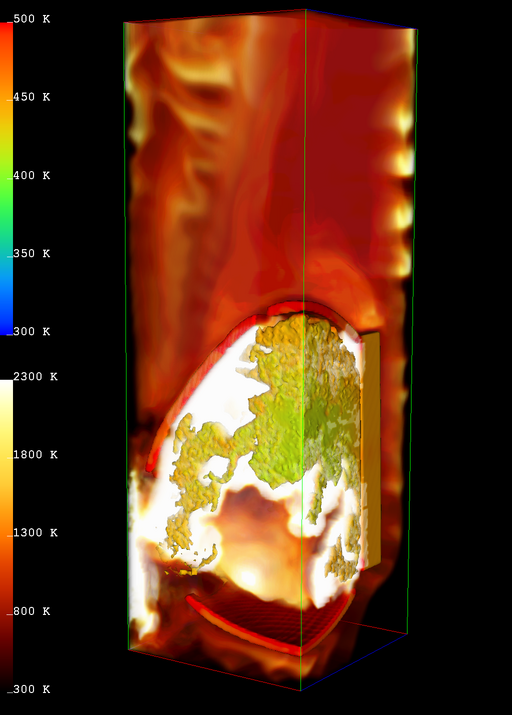
\includegraphics[width=\paperwidth,height=\paperheight,%
keepaspectratio]{fire-container-explosion-scirun.png}%
\vfill
}}}

%-------------------------------------------------------
% Versioning
%-------------------------------------------------------
\makeatletter
\def\MyYear#1{%
  \def\yy@##1##2##3##4;{##3##4}%
  \expandafter\yy@#1;
}
\def\MyMonth#1{%
  \def\yy@##1;{0##1}%
  \def\yy@##1##2;{##1##2}%
  \expandafter\yy@#1;
}
\def\MyDay#1{%
  \def\yy@##1;{0##1}%
  \def\yy@##1##2;{##1##2}%
  \expandafter\yy@#1;
}
\makeatother
\newcommand{\version}{Version \MyYear{\the\year}.\MyMonth{\the\month}.\MyDay{\the\day}}



%----------------------------------------------------------------------------------------
%	VARIOUS REQUIRED PACKAGES
%----------------------------------------------------------------------------------------

\usepackage{titlesec} % Allows customization of titles

%\usepackage{graphicx} % Required for including pictures
%\graphicspath{{./Pictures/}} % Specifies the directory where pictures are stored

\usepackage{lipsum} % Inserts dummy text

\usepackage{tikz} % Required for drawing custom shapes

\usepackage[english]{babel} % English language/hyphenation

\usepackage{enumitem} % Customize lists
\setlist{nolistsep} % Reduce spacing between bullet points and numbered lists

\usepackage{booktabs} % Required for nicer horizontal rules in tables

\usepackage{eso-pic} % Required for specifying an image background in the title page

%----------------------------------------------------------------------------------------
%	MAIN TABLE OF CONTENTS
%----------------------------------------------------------------------------------------

\usepackage{titletoc} % Required for manipulating the table of contents

\contentsmargin{0cm} % Removes the default margin

% Chapter text styling
\titlecontents{chapter}[1.25cm] % Indentation
{\addvspace{15pt}\large\sffamily\bfseries} % Spacing and font options for chapters
{\color{ocre!60}\contentslabel[\Large\thecontentslabel]{1.25cm}\color{ocre}} % Chapter number
{}  
{\color{ocre!60}\normalsize\sffamily\bfseries\;\titlerule*[.5pc]{.}\;\thecontentspage} % Page number

% Section text styling
\titlecontents{section}[1.55cm] % Indentation
{\addvspace{5pt}\sffamily} % Spacing and font options for sections
{\contentslabel[\thecontentslabel]{1.25cm}} % Section number
{}
{\sffamily\hfill\color{black}\thecontentspage} % Page number
[]

% Subsection text styling
\titlecontents{subsection}[1.85cm] % Indentation
{\addvspace{1pt}\sffamily\small} % Spacing and font options for subsections
{\contentslabel[\thecontentslabel]{1.25cm}} % Subsection number
{}
{\sffamily\;\titlerule*[.5pc]{.}\;\thecontentspage} % Page number
[] 

%----------------------------------------------------------------------------------------
%	MINI TABLE OF CONTENTS IN CHAPTER HEADS
%----------------------------------------------------------------------------------------

% Section text styling
\titlecontents{lsection}[0em] % Indendating
{\footnotesize\sffamily} % Font settings
{}
{}
{}

% Subsection text styling
\titlecontents{lsubsection}[.5em] % Indentation
{\normalfont\footnotesize\sffamily} % Font settings
{}
{}
{}
 
%----------------------------------------------------------------------------------------
%	PAGE HEADERS
%----------------------------------------------------------------------------------------

\usepackage{fancyhdr} % Required for header and footer configuration

\pagestyle{fancy}
\renewcommand{\chaptermark}[1]{\markboth{\sffamily\normalsize\bfseries #1}{}} % Chapter text font settings
\renewcommand{\sectionmark}[1]{\markright{\sffamily\normalsize\thesection\hspace{5pt}#1}{}} % Section text font settings
\fancyhf{} \fancyhead[LE,RO]{\sffamily\normalsize\thepage} % Font setting for the page number in the header
\fancyhead[LO]{\rightmark} % Print the nearest section name on the left side of odd pages
\fancyhead[RE]{\leftmark} % Print the current chapter name on the right side of even pages
\renewcommand{\headrulewidth}{0.5pt} % Width of the rule under the header
\addtolength{\headheight}{2.5pt} % Increase the spacing around the header slightly
\renewcommand{\footrulewidth}{0pt} % Removes the rule in the footer
\fancypagestyle{plain}{\fancyhead{}\renewcommand{\headrulewidth}{0pt}} % Style for when a plain pagestyle is specified

% Removes the header from odd empty pages at the end of chapters
\makeatletter
\renewcommand{\cleardoublepage}{
\clearpage\ifodd\c@page\else
\hbox{}
\vspace*{\fill}
\thispagestyle{empty}
\newpage
\fi}

%----------------------------------------------------------------------------------------
%	THEOREM STYLES
%----------------------------------------------------------------------------------------

\usepackage{amsmath} % For including math equations, theorems, symbols, etc
\usepackage{amsfonts} % For including math equations, theorems, symbols, etc
%\usepackage{amssymb} % For including math equations, theorems, symbols, etc
\usepackage{amsthm} % For including math equations, theorems, symbols, etc

\newcommand{\intoo}[2]{\mathopen{]}#1\,;#2\mathclose{[}}
\newcommand{\ud}{\mathop{\mathrm{{}d}}\mathopen{}}
\newcommand{\intff}[2]{\mathopen{[}#1\,;#2\mathclose{]}}
\newtheorem{notation}{Notation}[chapter]

\newtheoremstyle{ocrenum} % Theorem style name
{7pt} % Space above
{7pt} % Space below
{\normalfont} % Body font
{} % Indent amount
{\small\bf\sffamily\color{ocre}} % Theorem head font
{\;\;} % Punctuation after theorem head
{0.25em} % Space after theorem head
{\small\sffamily\color{ocre}\thmname{#1}\thmnumber{\@ifnotempty{#1}{ }\@upn{#2}} % Theorem text (e.g. Theorem 2.1)
\thmnote{\ {\the\thm@notefont\sffamily\bfseries\color{black}--- #3.}}} % Optional theorem note
\renewcommand{\qedsymbol}{$\blacksquare$} % Optional qed square

\newtheoremstyle{blacknumex} % Theorem style name
{7pt} % Space above
{7pt} % Space below
{\normalfont} % Body font
{} % Indent amount
{\small\bf\sffamily} % Theorem head font
{\;\;} % Punctuation after theorem head
{0.25em} % Space after theorem head
{\small\sffamily{\tiny\ensuremath{\blacksquare}}\ \thmname{#1}\thmnumber{\@ifnotempty{#1}{ }\@upn{#2}} % Theorem text (e.g. Theorem 2.1)
\thmnote{\ {\the\thm@notefont\sffamily\bfseries--- #3.}}} % Optional theorem note

\newtheoremstyle{blacknum} % Theorem style name
{7pt} % Space above
{7pt} % Space below
{\normalfont} % Body font
{} % Indent amount
{\small\bf\sffamily} % Theorem head font
{\;\;} % Punctuation after theorem head
{0.25em} % Space after theorem head
{\small\sffamily\thmname{#1}\thmnumber{\@ifnotempty{#1}{ }\@upn{#2}} % Theorem text (e.g. Theorem 2.1)
\thmnote{\ {\the\thm@notefont\sffamily\bfseries--- #3.}}} % Optional theorem note
\makeatother

% Defines the theorem text style for each type of theorem to one of the three styles above
\theoremstyle{ocrenum}
\newtheorem{theoremeT}{Theorem}[chapter]
\newtheorem{proposition}{Proposition}[chapter]
\newtheorem{problem}{Problem}[chapter]
\newtheorem{exerciseT}{Exercise}[chapter]
\theoremstyle{blacknumex}
\newtheorem{exampleT}{Example}[chapter]
\theoremstyle{blacknum}
\newtheorem{vocabulary}{Vocabulary}[chapter]
\newtheorem{definitionT}{Definition}[chapter]
\newtheorem{corollaryT}{Corollary}[chapter]

%----------------------------------------------------------------------------------------
%	DEFINITION OF COLORED BOXES
%----------------------------------------------------------------------------------------

\RequirePackage[framemethod=default]{mdframed} % Required for creating the theorem, definition, exercise and corollary boxes

% Theorem box
\newmdenv[skipabove=7pt,
skipbelow=7pt,
backgroundcolor=black!5,
linecolor=ocre,
innerleftmargin=5pt,
innerrightmargin=5pt,
innertopmargin=5pt,
leftmargin=0cm,
rightmargin=0cm,
innerbottommargin=5pt]{tBox}

% Exercise box	  
\newmdenv[skipabove=7pt,
skipbelow=7pt,
rightline=false,
leftline=true,
topline=false,
bottomline=false,
backgroundcolor=ocre!10,
linecolor=ocre,
innerleftmargin=5pt,
innerrightmargin=5pt,
innertopmargin=5pt,
innerbottommargin=5pt,
leftmargin=0cm,
rightmargin=0cm,
linewidth=4pt]{eBox}	

% Definition box
\newmdenv[skipabove=10pt,
skipbelow=10pt,
rightline=false,
leftline=true,
topline=false,
bottomline=false,
linecolor=ocre,
innerleftmargin=5pt,
innerrightmargin=5pt,
innertopmargin=0pt,
leftmargin=0cm,
rightmargin=0cm,
linewidth=4pt,
innerbottommargin=0pt]{dBox}	

% Corollary box
\newmdenv[skipabove=7pt,
skipbelow=7pt,
rightline=false,
leftline=true,
topline=false,
bottomline=false,
linecolor=gray,
backgroundcolor=black!5,
innerleftmargin=5pt,
innerrightmargin=5pt,
innertopmargin=5pt,
leftmargin=0cm,
rightmargin=0cm,
linewidth=4pt,
innerbottommargin=5pt]{cBox}				  
		  

% Creates an environment for each type of theorem and assigns it a theorem text style from the "Theorem Styles" section above and a colored box from above
\newenvironment{theorem}{\begin{tBox}\begin{theoremeT}}{\end{theoremeT}\end{tBox}}
\newenvironment{exercise}{\begin{eBox}\begin{exerciseT}}{\hfill{\color{ocre}\tiny\ensuremath{\blacksquare}}\end{exerciseT}\end{eBox}}				  
\newenvironment{definition}{\begin{dBox}\begin{definitionT}}{\end{definitionT}\end{dBox}}	
\newenvironment{example}{\begin{exampleT}}{\hfill{\tiny\ensuremath{\blacksquare}}\end{exampleT}}		
\newenvironment{corollary}{\begin{cBox}\begin{corollaryT}}{\end{corollaryT}\end{cBox}}	

%----------------------------------------------------------------------------------------
%	REMARK ENVIRONMENT
%----------------------------------------------------------------------------------------

\newenvironment{remark}{\par\vskip10pt\small % Vertical white space above the remark and smaller font size
\begin{list}{}{
\leftmargin=35pt % Indentation on the left
\rightmargin=25pt}\item\ignorespaces % Indentation on the right
\makebox[-2.5pt]{\begin{tikzpicture}[overlay]
\node[draw=ocre!60,line width=1pt,circle,fill=ocre!25,font=\sffamily\bfseries,inner sep=2pt,outer sep=0pt] at (-15pt,0pt){\textcolor{ocre}{R}};\end{tikzpicture}} % Orange R in a circle
\advance\baselineskip -1pt}{\end{list}\vskip5pt} % Tighter line spacing and white space after remark

%----------------------------------------------------------------------------------------
%	SECTION NUMBERING IN THE MARGIN
%----------------------------------------------------------------------------------------

\makeatletter
\renewcommand{\@seccntformat}[1]{\llap{\textcolor{ocre}{\csname the#1\endcsname}\hspace{1em}}}                    
\renewcommand{\section}{\@startsection{section}{1}{\z@}
{-4ex \@plus -1ex \@minus -.4ex}
{1ex \@plus.2ex }
{\normalfont\large\sffamily\bfseries}}
\renewcommand{\subsection}{\@startsection {subsection}{2}{\z@}
{-3ex \@plus -0.1ex \@minus -.4ex}
{0.5ex \@plus.2ex }
{\normalfont\sffamily\bfseries}}
\renewcommand{\subsubsection}{\@startsection {subsubsection}{3}{\z@}
{-2ex \@plus -0.1ex \@minus -.2ex}
{0.2ex \@plus.2ex }
{\color{teal}\normalfont\small\sffamily\bfseries}}                        
\renewcommand\paragraph{\@startsection{paragraph}{4}{\z@}
{-2ex \@plus-.2ex \@minus .2ex}
{0.1ex}
{\normalfont\small\sffamily\bfseries}}

%----------------------------------------------------------------------------------------
%	CHAPTER HEADINGS
%----------------------------------------------------------------------------------------

\newcommand{\thechapterimage}{}
\newcommand{\chapterimage}[1]{\renewcommand{\thechapterimage}{#1}}
\def\thechapter{\arabic{chapter}}
\def\@makechapterhead#1{
\thispagestyle{empty}
{\centering \normalfont\sffamily
\ifnum \c@secnumdepth >\m@ne
\if@mainmatter
\startcontents
\begin{tikzpicture}[remember picture,overlay]
\node at (current page.north west)
{\begin{tikzpicture}[remember picture,overlay]

\node[anchor=north west,inner sep=0pt] at (14,-0.5) {\includegraphics[width=0.3\paperwidth]{\thechapterimage}};

%Commenting the 3 lines below removes the small contents box in the chapter heading
%\draw[fill=white,opacity=.6] (1cm,0) rectangle (8cm,-7cm);
%\node[anchor=north west] at (1cm,.25cm) {\parbox[t][8cm][t]{6.5cm}{\huge\bfseries\flushleft \printcontents{l}{1}{\setcounter{tocdepth}{2}}}};

\draw[anchor=west] (5cm,-8cm) node [rounded corners=25pt,fill=white,fill opacity=1.0,text opacity=1,draw=ocre,draw opacity=1,line width=2pt,inner sep=15pt]{\huge\sffamily\bfseries\textcolor{black}{\thechapter\ ---\ #1\vphantom{plPQq}\makebox[22cm]{}}};
\end{tikzpicture}};
\end{tikzpicture}}\par\vspace*{200\p@}
\fi
\fi
}
\def\@makeschapterhead#1{
\thispagestyle{empty}
{\centering \normalfont\sffamily
\ifnum \c@secnumdepth >\m@ne
\if@mainmatter
\startcontents
\begin{tikzpicture}[remember picture,overlay]
\node at (current page.north west)
{\begin{tikzpicture}[remember picture,overlay]
\node[anchor=north west] at (14,-0.5) {\includegraphics[width=0.3\paperwidth]{\thechapterimage}};
\draw[anchor=west] (5cm,-8cm) node [rounded corners=25pt,fill=white,opacity=.7,inner sep=15.5pt]{\huge\sffamily\bfseries\textcolor{black}{\vphantom{plPQq}\makebox[22cm]{}}};
\draw[anchor=west] (5cm,-8cm) node [rounded corners=25pt,draw=ocre,line width=2pt,inner sep=15pt]{\huge\sffamily\bfseries\textcolor{black}{#1\vphantom{plPQq}\makebox[22cm]{}}};
\end{tikzpicture}};
\end{tikzpicture}}\par\vspace*{200\p@}
\fi
\fi
}
\makeatother

\newcommand{\AuthorNote}[1]{{\color{authorNoteColor} \sffamily{\textbf{#1}}}}

\newcommand{\Vaango}{\textsc{Vaango}\,}
\newcommand{\Uintah}{\textsc{Uintah}\,}
\newcommand{\MPM}{\textsc{MPM}\,}
\newcommand{\ICE}{\textsc{ICE}\,}
\newcommand{\MPMICE}{\textsc{MPMICE}\,}
\newcommand{\Arena}{\textsc{Arena}\,}
\newcommand{\Visit}{\textsc{VisIt}\,}
\newcommand{\Parsim}{\textsc{ParSim}\,}
\newcommand{\Textsfc}[1]{{\OliveD \textsf{#1}}\,}
\newcommand{\Textbfc}[1]{{\Pink \textsf{#1}}\,}
\newcommand{\Textttc}[1]{{\DarkGreen \texttt{#1}}\,}

%Wide bar
\newcommand{\overbar}[1]{\mkern 1.5mu\overline{\mkern-1.5mu#1\mkern-1.5mu}\mkern 1.5mu}
\renewcommand{\bar}[1]{\overbar{#1}}
\renewcommand{\widehat}[1]{\hat{#1}}

%__________________________________
% new commands for all sections
\newcommand{\BBComment}[1]{ \marginpar{{\scriptsize \color{red} #1 }}}
\newcommand{\red}[1]{\color{red} {#1} \color{black}}
\newcommand{\TT}[1]{\ensuremath{\tt{#1}\normalfont}}

% MPM & ICE
\newcommand{\tn}[1]{\mbox{\ensuremath{\mathbf{#1}}}}
\newcommand{\sig}{\mbox{\boldmath $\sigma \!\!$ \unboldmath}}
\newcommand{\bnabla} {\mbox {\boldmath $\nabla \!\!$ \unboldmath}}
\newcommand{\taubold} {\mbox{\boldmath $\tau \!\!$ \unboldmath}}
\newcommand{\f}{\ensuremath{f^{\theta}_r} }

\newcommand{\Texp}{\rm{exp}}
\newcommand{\Delt}{\ensuremath{\Delta t}}
\newcommand{\Epj}{\ensuremath{\epsilon_{p,j}}}
\newcommand{\Epo}{\ensuremath{\epsilon_{p,0}}}
\newcommand{\lambdadot}{\ensuremath{\dot{\lambda}}}
\def\bfE{{\bf E}}

\newcommand{\hangp}[1]{\makebox[0pt][r]{(}#1\makebox[0pt][l]{)}} % New command to create parentheses around text in tables which take up no horizontal space - this improves column spacing
\newcommand{\hangstar}{\makebox[0pt][l]{*}} % New command to create asterisks in tables which take up no horizontal space - this improves column spacing

\newcommand{\monthyear}{\ifcase\month\or January\or February\or March\or April\or May\or June\or July\or August\or September\or October\or November\or December\fi\space\number\year} % A command to print the current month and year

\newcommand{\blankpage}{\newpage\hbox{}\thispagestyle{empty}\newpage} % Command to insert a blank page

\def\rmd{{\rm d}}
\def\rme{{\rm e}}
\def\rmf{{\rm f}}
\def\rmr{{\rm r}}
\def\rmR{{\rm R}}
\def\rms{{\rm s}}
\def\bfd{{\bf d}}
\def\bfE{{\bf E}}
\def\bfF{{\bf F}}
\def\bff{{\bf f}}
\def\bfg{{\bf g}}
\def\bfI{{\bf I}}
\def\bfj{{\bf j}}
\def\bfm{{\bf m}}
\def\bfr{{\bf r}}
\def\bfx{{\bf x}}
\def\bfu{{\bf u}}
\def\rmg{{\rm g}}
\def\bfa{{\bf a}}
\def\bfG{{\bf G}}
\def\bfv{{\bf v}}
\def\tdot{{\textstyle\cdot}}

\pdfcompresslevel=9
%\raggedright

\newcommand{\handout}[3]{
        \begin{center}
         % \copyright 
          Biswajit Banerjee \hspace{4.2in} University of Utah\\
          \vspace{10pt}
          {\Large\bf Waves in Composites and Metamaterials}\\
          \vspace{6pt}
          (Instructor: Prof. G. W. Milton)
        \end{center}
        \vspace{8pt}\noindent
        %\begin{center}
        {\underline{\makebox[7.0in]{\large\bf\noindent
                \makebox[1.5in][l]{#1~~~} \hfill {~~~#2~~~} \hfill
                \makebox[1.5in][r]{~~~#3}}}}
        %\end{center}
        }

\newcommand{\heading}[1]{
        \begin{center}{\large\bf{#1}}\end{center}}

\newcommand{\subheading}[1]{
        \begin{center}{\normalsize\bf{#1}}\end{center}}

\newcommand{\subsubheading}[1]{
        \begin{center}{\small\bf{#1}}\end{center}}

\newcommand{\Heading}[1]{
        \vspace{12pt}\begin{center}{\Large\bf{#1}}\end{center}}

\newcommand{\Subheading}[1]{
        \vspace{8pt}\begin{center}{\large\bf{#1}}\end{center}}

\newcommand{\Jump}[1]{\ensuremath{\llbracket#1\rrbracket}}
\newcommand{\Blimitx}[1]{\ensuremath{\left[#1\right]_{x_a}^{x_b}}}
\newcommand{\Deriv}[2]{\ensuremath{\cfrac{d#1}{d#2}}}
\newcommand{\MDeriv}[2]{\ensuremath{\cfrac{D#1}{D#2}}}
\newcommand{\DDeriv}[2]{\ensuremath{\cfrac{d^2#1}{d#2^2}}}
\newcommand{\DDDeriv}[2]{\ensuremath{\cfrac{d^3#1}{d#2^3}}}
\newcommand{\DDDDeriv}[2]{\ensuremath{\cfrac{d^4#1}{d#2^4}}}
\newcommand{\Intx}{\ensuremath{\int_{x_a}^{x_b}}}
\newcommand{\IntX}{\ensuremath{\int_{X_a}^{X_b}}}
\newcommand{\Intiso}{\ensuremath{\int_{-1}^{1}}}
\newcommand{\IntOmegaA}{\ensuremath{\int_{\Omega_0}}}
\newcommand{\IntOmega}{\ensuremath{\int_{\Omega}}}
\newcommand{\IntDOmega}{\ensuremath{\int_{\partial\Omega}}}
\newcommand{\Norm}[2]{\ensuremath{\left\lVert#1\right\rVert_{#2}}}
\newcommand{\norm}[1]{\ensuremath{\left\lVert#1\right\rVert}}
\newcommand{\Var}[1]{\ensuremath{\delta #1}}
\newcommand{\DelT}{\ensuremath{\Delta t}}
\newcommand{\CalA}{\ensuremath{\mathcal{A}}}
\newcommand{\CalB}{\ensuremath{\mathcal{B}}}
\newcommand{\CalC}{\ensuremath{\mathcal{C}}}
\newcommand{\CalF}{\ensuremath{\mathcal{F}}}
\newcommand{\CalL}{\ensuremath{\mathcal{L}}}
\newcommand{\CalM}{\ensuremath{\mathcal{M}}}
\newcommand{\BCalM}{\ensuremath{\boldsymbol{\CalM}}}
\newcommand{\CalN}{\ensuremath{\mathcal{N}}}
\newcommand{\CalP}{\ensuremath{\mathcal{P}}}
\newcommand{\CalS}{\ensuremath{\mathcal{S}}}
\newcommand{\BCalS}{\ensuremath{\boldsymbol{\CalS}}}
\newcommand{\CalT}{\ensuremath{\mathcal{T}}}
\newcommand{\CalV}{\ensuremath{\mathcal{V}}}
\newcommand{\CalW}{\ensuremath{\mathcal{W}}}
\newcommand{\CalX}{\ensuremath{\mathcal{X}}}
\newcommand{\Comp}[2]{\ensuremath{#1 \circ #2}}
\newcommand{\Map}[3]{\ensuremath{#1 : #2 \rightarrow #3}}
\newcommand{\MapTo}[3]{\ensuremath{#1 : #2 \mapsto #3}}
\newcommand{\Real}[1]{\ensuremath{\mathbb{R}^{#1}}}
\newcommand{\Ve}{\ensuremath{\varepsilon}}
\newcommand{\BHat}[1]{\ensuremath{\widehat{\boldsymbol{#1}}}}
\newcommand{\BTx}{\ensuremath{\tilde{\boldsymbol{x}}}}
\newcommand{\Beh}{\ensuremath{\hat{\boldsymbol{e}}}}
\newcommand{\BHex}{\ensuremath{\hat{\boldsymbol{e}}_1}}
\newcommand{\BHey}{\ensuremath{\hat{\boldsymbol{e}}_2}}
\newcommand{\BHez}{\ensuremath{\hat{\boldsymbol{e}}_3}}
\newcommand{\BHn}[1]{\ensuremath{\hat{\boldsymbol{n}}_{#1}}}
\newcommand{\BHe}[1]{\ensuremath{\hat{\boldsymbol{e}}_{#1}}}
\newcommand{\BHg}[1]{\ensuremath{\hat{\boldsymbol{g}}_{#1}}}
\newcommand{\BHG}[1]{\ensuremath{\hat{\boldsymbol{G}}_{#1}}}
\newcommand{\Hn}{\ensuremath{\hat{\boldsymbol{n}}}}
\newcommand{\Mba}{\ensuremath{\mathbf{a}}}
\newcommand{\Mbatilde}{\ensuremath{\widetilde{\mathbf{a}}}}
\newcommand{\Mbb}{\ensuremath{\mathbf{b}}}
\newcommand{\Mbd}{\ensuremath{\mathbf{d}}}
\newcommand{\Mbf}{\ensuremath{\mathbf{f}}}
\newcommand{\Mbn}{\ensuremath{\mathbf{n}}}
\newcommand{\Mbntilde}{\ensuremath{\widetilde{\mathbf{n}}}}
\newcommand{\Mbr}{\ensuremath{\mathbf{r}}}
\newcommand{\Mbu}{\ensuremath{\mathbf{u}}}
\newcommand{\Mbv}{\ensuremath{\mathbf{v}}}
\newcommand{\Mbx}{\ensuremath{\mathbf{x}}}
\newcommand{\MbA}{\ensuremath{\mathbf{A}}}
\newcommand{\MbB}{\ensuremath{\mathbf{B}}}
\newcommand{\MbC}{\ensuremath{\mathbf{C}}}
\newcommand{\MbD}{\ensuremath{\mathbf{D}}}
\newcommand{\MbH}{\ensuremath{\mathbf{H}}}
\newcommand{\MbHbar}{\ensuremath{\mathbf{\overline{H}}}}
\newcommand{\MbI}{\ensuremath{\mathbf{I}}}
\newcommand{\MbK}{\ensuremath{\mathbf{K}}}
\newcommand{\MbKbar}{\ensuremath{\overline{\mathbf{K}}}}
\newcommand{\MbKtilde}{\ensuremath{\widetilde{\mathbf{K}}}}
\newcommand{\MbM}{\ensuremath{\mathbf{M}}}
\newcommand{\MbN}{\ensuremath{\mathbf{N}}}
\newcommand{\MbP}{\ensuremath{\mathbf{P}}}
\newcommand{\MbPbar}{\ensuremath{\overline{\mathbf{P}}}}
\newcommand{\MbR}{\ensuremath{\mathbf{R}}}
\newcommand{\MbT}{\ensuremath{\mathbf{T}}}
\newcommand{\MbU}{\ensuremath{\mathbf{U}}}
\newcommand{\MbV}{\ensuremath{\mathbf{V}}}
\newcommand{\MbX}{\ensuremath{\mathbf{X}}}
\newcommand{\MbSig}{\ensuremath{\boldsymbol{\sigma}}}
\newcommand{\Mbone}{\ensuremath{\mathbf{1}}}
\newcommand{\Mbzero}{\ensuremath{\mathbf{0}}}
%\newcommand{\Mb}{\ensuremath{\left[\mathsf{b}\right]}}
%\newcommand{\Mu}{\ensuremath{\left[\mathsf{u}\right]}}
%\newcommand{\Mv}{\ensuremath{\left[\mathsf{v}\right]}}
%\newcommand{\Mw}{\ensuremath{\left[\mathsf{w}\right]}}
%\newcommand{\Mx}{\ensuremath{\left[\mathsf{x}\right]}}
\newcommand{\MA}{\ensuremath{\left[\mathsf{A}\right]}}
\newcommand{\MB}{\ensuremath{\left[\mathsf{B}\right]}}
\newcommand{\MC}{\ensuremath{\left[\mathsf{C}\right]}}
\newcommand{\MD}{\ensuremath{\left[\mathsf{D}\right]}}
\newcommand{\MH}{\ensuremath{\left[\mathsf{H}\right]}}
\newcommand{\MI}{\ensuremath{\left[\mathsf{I}\right]}}
\newcommand{\ML}{\ensuremath{\left[\mathsf{L}\right]}}
\newcommand{\MM}{\ensuremath{\left[\mathsf{M}\right]}}
\newcommand{\MN}{\ensuremath{\left[\mathsf{N}\right]}}
\newcommand{\MP}{\ensuremath{\left[\mathsf{P}\right]}}
\newcommand{\MQ}{\ensuremath{\left[\mathsf{Q}\right]}}
\newcommand{\MR}{\ensuremath{\left[\mathsf{R}\right]}}
\newcommand{\MT}{\ensuremath{\left[\mathsf{T}\right]}}
\newcommand{\MV}{\ensuremath{\left[\mathsf{V}\right]}}
%\newcommand{\Mone}{\ensuremath{\left[\mathsf{1}\right]}}
%\newcommand{\Mzero}{\ensuremath{\left[\mathsf{0}\right]}}
\newcommand{\SfA}{\ensuremath{\boldsymbol{\mathsf{A}}}}
\newcommand{\SfB}{\ensuremath{\boldsymbol{\mathsf{B}}}}
\newcommand{\SfC}{\ensuremath{\boldsymbol{\mathsf{C}}}}
\newcommand{\SfD}{\ensuremath{\boldsymbol{\mathsf{D}}}}
\newcommand{\SfI}{\ensuremath{\boldsymbol{\mathsf{I}}}}
\newcommand{\SfL}{\ensuremath{\boldsymbol{\mathsf{L}}}}
\newcommand{\Sfp}{\ensuremath{\boldsymbol{\mathsf{p}}}}
\newcommand{\SfP}{\ensuremath{\boldsymbol{\mathsf{P}}}}
\newcommand{\SfS}{\ensuremath{\boldsymbol{\mathsf{S}}}}
\newcommand{\SfT}{\ensuremath{\boldsymbol{\mathsf{T}}}}
\newcommand{\Msig}{\ensuremath{\left[\boldsymbol{\sigma}\right]}}
\newcommand{\Meps}{\ensuremath{\left[\boldsymbol{\varepsilon}\right]}}
\newcommand{\Ex}{\ensuremath{\boldsymbol{e}_1}}
\newcommand{\Ey}{\ensuremath{\boldsymbol{e}_2}}
\newcommand{\Ez}{\ensuremath{\boldsymbol{e}_3}}
\newcommand{\Exp}{\ensuremath{\boldsymbol{e}^{'}_1}}
\newcommand{\Eyp}{\ensuremath{\boldsymbol{e}^{'}_2}}
\newcommand{\Ezp}{\ensuremath{\boldsymbol{e}^{'}_3}}
\newcommand{\Ep}{\ensuremath{\varepsilon_p}}
\newcommand{\Epi}{\ensuremath{\varepsilon_{pi}}}
\newcommand{\Epdot}[1]{\ensuremath{\dot{\varepsilon}_{p#1}}}
\newcommand{\Epsxx}{\ensuremath{\varepsilon_{11}}}
\newcommand{\Epsyy}{\ensuremath{\varepsilon_{22}}}
\newcommand{\Epszz}{\ensuremath{\varepsilon_{33}}}
\newcommand{\Epsyz}{\ensuremath{\varepsilon_{23}}}
\newcommand{\Epszx}{\ensuremath{\varepsilon_{31}}}
\newcommand{\Epsxy}{\ensuremath{\varepsilon_{12}}}
\newcommand{\Sigxx}{\ensuremath{\sigma_{11}}}
\newcommand{\Sigyy}{\ensuremath{\sigma_{22}}}
\newcommand{\Sigzz}{\ensuremath{\sigma_{33}}}
\newcommand{\Sigyz}{\ensuremath{\sigma_{23}}}
\newcommand{\Sigzx}{\ensuremath{\sigma_{31}}}
\newcommand{\Sigxy}{\ensuremath{\sigma_{12}}}
\newcommand{\Eps}[1]{\ensuremath{\varepsilon_{#1}}}
\newcommand{\Sig}[1]{\ensuremath{\sigma_{#1}}}
\newcommand{\X}{\ensuremath{X_1}}
\newcommand{\Y}{\ensuremath{X_2}}
\newcommand{\Z}{\ensuremath{X_3}}
\newcommand{\erf}{\text{erf}}
\newcommand{\Xidot}{\ensuremath{\dot{\xi}}}
\newcommand{\Balpha}{\ensuremath{\boldsymbol{\alpha}}}
\newcommand{\Balphahat}{\ensuremath{\widehat{\boldsymbol{\alpha}}}}
\newcommand{\Bbeta}{\ensuremath{\boldsymbol{\beta}}}
\newcommand{\Beta}{\ensuremath{\boldsymbol{\eta}}}
\newcommand{\Bchi}{\ensuremath{\boldsymbol{\chi}}}
\newcommand{\Bpsi}{\ensuremath{\boldsymbol{\psi}}}
\newcommand{\Bveps}{\ensuremath{\boldsymbol{\varepsilon}}}
\newcommand{\BGamma}{\ensuremath{\boldsymbol{\mathit{\Gamma}}}}
\newcommand{\BGammahat}{\ensuremath{\boldsymbol{\mathit{\widehat{\Gamma}}}}}
%\newcommand{\BGammahat}{\ensuremath{\widehat{\BGamma}}}
\newcommand{\Bkappa}{\ensuremath{\boldsymbol{\kappa}}}
\newcommand{\Bbeps}{\ensuremath{\bar{\boldsymbol{\varepsilon}}}}
\newcommand{\Bnabla}{\ensuremath{\boldsymbol{\nabla}}}
\newcommand{\Bomega}{\ensuremath{\boldsymbol{\omega}}}
\newcommand{\BOmega}{\ensuremath{\boldsymbol{\Omega}}}
\newcommand{\Bsig}{\ensuremath{\boldsymbol{\sigma}}}
\newcommand{\Bsigbar}{\ensuremath{\overline{\boldsymbol{\sigma}}}}
\newcommand{\BSig}{\ensuremath{\boldsymbol{\Sigma}}}
\newcommand{\Btau}{\ensuremath{\boldsymbol{\tau}}}
\newcommand{\Bpi}{\ensuremath{\boldsymbol{\pi}}}
\newcommand{\Brho}{\ensuremath{\boldsymbol{\rho}}}
\newcommand{\Bvarphi}{\ensuremath{\boldsymbol{\varphi}}}
\newcommand{\phibar}{\ensuremath{\overline{\varphi}}}
\newcommand{\Blambda}{\ensuremath{\boldsymbol{\lambda}}}
\newcommand{\Btheta}{\ensuremath{\boldsymbol{\theta}}}
\newcommand{\Bthetav}{\ensuremath{\mathbf{\theta}}}
\newcommand{\Bgamma}{\ensuremath{\boldsymbol{\gamma}}}
\newcommand{\Bmu}{\ensuremath{\boldsymbol{\mu}}}
\newcommand{\Bxi}{\ensuremath{\boldsymbol{\xi}}}
\newcommand{\BPi}{\ensuremath{\boldsymbol{\Pi}}}
\newcommand{\Bone}{\ensuremath{\boldsymbol{\mathit{1}}}}
\newcommand{\Bonev}{\ensuremath{\boldsymbol{1}}}
\newcommand{\Bzero}{\ensuremath{\boldsymbol{0}}}
\newcommand{\BzeroT}{\ensuremath{\boldsymbol{\mathit{0}}}}
\newcommand{\Ba}{\ensuremath{\mathbf{a}}}
\newcommand{\Bb}{\ensuremath{\mathbf{b}}}
\newcommand{\BbT}{\ensuremath{\boldsymbol{b}}}
\newcommand{\Bc}{\ensuremath{\mathbf{c}}}
\newcommand{\Bd}{\ensuremath{\mathbf{d}}}
\newcommand{\BdT}{\ensuremath{\boldsymbol{d}}}
\newcommand{\Bdv}{\ensuremath{\mathbf{d}}}
\newcommand{\Be}{\ensuremath{\mathbf{e}}}
\newcommand{\BeT}{\ensuremath{\boldsymbol{e}}}
\newcommand{\Bf}{\ensuremath{\mathbf{f}}}
\newcommand{\Bg}{\ensuremath{\mathbf{g}}}
\newcommand{\Bh}{\ensuremath{\boldsymbol{h}}}
\newcommand{\Bhv}{\ensuremath{\mathbf{h}}}
\newcommand{\Bj}{\ensuremath{\mathbf{j}}}
\newcommand{\Bk}{\ensuremath{\mathbf{k}}}
\newcommand{\Bl}{\ensuremath{\mathbf{l}}}
\newcommand{\BlT}{\ensuremath{\boldsymbol{l}}}
\newcommand{\Bm}{\ensuremath{\mathbf{m}}}
\newcommand{\Bn}{\ensuremath{\mathbf{n}}}
\newcommand{\BnT}{\ensuremath{\boldsymbol{n}}}
\newcommand{\Bo}{\ensuremath{\mathbf{o}}}
\newcommand{\Bp}{\ensuremath{\mathbf{p}}}
\newcommand{\Bq}{\ensuremath{\mathbf{q}}}
\newcommand{\Br}{\ensuremath{\boldsymbol{r}}}
\newcommand{\Brv}{\ensuremath{\mathbf{r}}}
\newcommand{\Bs}{\ensuremath{\mathbf{s}}}
\newcommand{\BsT}{\ensuremath{\boldsymbol{s}}}
\newcommand{\Bsv}{\ensuremath{\mathbf{s}}}
\newcommand{\Bt}{\ensuremath{\mathbf{t}}}
\newcommand{\Bu}{\ensuremath{\mathbf{u}}}
\newcommand{\Bv}{\ensuremath{\mathbf{v}}}
\newcommand{\Bw}{\ensuremath{\mathbf{w}}}
\newcommand{\Bx}{\ensuremath{\mathbf{x}}}
\newcommand{\By}{\ensuremath{\mathbf{y}}}
\newcommand{\Bz}{\ensuremath{\mathbf{z}}}
\newcommand{\BA}{\ensuremath{\boldsymbol{A}}}
\newcommand{\BB}{\ensuremath{\boldsymbol{B}}}
\newcommand{\BBbar}{\ensuremath{\bar{\boldsymbol{B}}}}
\newcommand{\BC}{\ensuremath{\boldsymbol{C}}}
\newcommand{\BCbar}{\ensuremath{\bar{\boldsymbol{C}}}}
\newcommand{\Cbar}{\ensuremath{\bar{C}}}
\newcommand{\BD}{\ensuremath{\boldsymbol{D}}}
\newcommand{\BE}{\ensuremath{\boldsymbol{E}}}
\newcommand{\BF}{\ensuremath{\boldsymbol{F}}}
\newcommand{\BFbar}{\ensuremath{\bar{\boldsymbol{F}}}}
\newcommand{\Fbar}{\ensuremath{\bar{F}}}
\newcommand{\BG}{\ensuremath{\boldsymbol{G}}}
\newcommand{\BGv}{\ensuremath{\mathbf{G}}}
\newcommand{\BH}{\ensuremath{\boldsymbol{H}}}
\newcommand{\BI}{\ensuremath{\boldsymbol{I}}}
\newcommand{\BBI}{\ensuremath{\mathbb{I}}}
\newcommand{\BJ}{\ensuremath{\boldsymbol{J}}}
\newcommand{\BK}{\ensuremath{\boldsymbol{K}}}
\newcommand{\BL}{\ensuremath{\boldsymbol{L}}}
\newcommand{\BM}{\ensuremath{\boldsymbol{M}}}
\newcommand{\BNv}{\ensuremath{\mathbf{N}}}
\newcommand{\BN}{\ensuremath{\boldsymbol{N}}}
\newcommand{\BP}{\ensuremath{\boldsymbol{P}}}
\newcommand{\BBP}{\ensuremath{\mathbb{P}}}
\newcommand{\BQ}{\ensuremath{\boldsymbol{Q}}}
\newcommand{\BBQ}{\ensuremath{\mathbb{Q}}}
\newcommand{\BQv}{\ensuremath{\mathbf{Q}}}
\newcommand{\BR}{\ensuremath{\boldsymbol{R}}}
\newcommand{\BBR}{\ensuremath{\mathbb{R}}}
\newcommand{\BS}{\ensuremath{\boldsymbol{S}}}
\newcommand{\BSmat}{\ensuremath{\mathbf{S}}}
\newcommand{\BT}{\ensuremath{\boldsymbol{T}}}
\newcommand{\BTv}{\ensuremath{\mathbf{T}}}
\newcommand{\BU}{\ensuremath{\boldsymbol{U}}}
\newcommand{\BV}{\ensuremath{\boldsymbol{V}}}
\newcommand{\BW}{\ensuremath{\boldsymbol{W}}}
\newcommand{\BX}{\ensuremath{\mathbf{X}}}
\newcommand{\BXT}{\ensuremath{\boldsymbol{X}}}
\newcommand{\BY}{\ensuremath{\boldsymbol{Y}}}
\newcommand{\BZ}{\ensuremath{\boldsymbol{Z}}}
\newcommand{\Trial}{\ensuremath{\text{trial}}}
\newcommand{\Tiso}{\ensuremath{\text{iso}}}
\newcommand{\Tint}{\ensuremath{\text{int}}}
\newcommand{\Text}{\ensuremath{\text{ext}}}
\newcommand{\Tkin}{\ensuremath{\text{kin}}}
\newcommand{\Tbody}{\ensuremath{\text{body}}}
\newcommand{\Tinert}{\ensuremath{\text{inertial}}}
\newcommand{\Telast}{\ensuremath{\text{elastic}}}
\newcommand{\Ttop}{\ensuremath{\text{top}}}
\newcommand{\Tbot}{\ensuremath{\text{bot}}}
\newcommand{\Tcore}{\ensuremath{\text{core}}}
\newcommand{\Teq}{\ensuremath{\text{eq}}}
\newcommand{\Tface}{\ensuremath{\text{face}}}
\newcommand{\Tpot}{\ensuremath{\text{pot}}}
\newcommand{\Tright}{\ensuremath{\text{right}}}
\newcommand{\Tleft}{\ensuremath{\text{left}}}
\newcommand{\Tdrag}{\ensuremath{\text{drag}}}
\newcommand{\Tmin}{\ensuremath{\text{min}}}
\newcommand{\Tmax}{\ensuremath{\text{max}}}
\newcommand{\Tsat}{\ensuremath{\text{sat}}}
\newcommand{\Tapex}{\ensuremath{\text{apex}}}
\newcommand{\Tref}{\ensuremath{\text{ref}}}
\newcommand{\Tnew}{\ensuremath{\text{new}}}
\newcommand{\Told}{\ensuremath{\text{old}}}
\newcommand{\Tin}{\ensuremath{\text{in}}}
\newcommand{\Tlocal}{\ensuremath{\text{local}}}
\newcommand{\Tmid}{\ensuremath{\text{mid}}}
\newcommand{\Tout}{\ensuremath{\text{out}}}
\newcommand{\Tratio}{\ensuremath{\text{ratio}}}
\newcommand{\Tsub}{\ensuremath{\text{sub}}}
\newcommand{\Te}{\ensuremath{\text{e}}}
\newcommand{\Tp}{\ensuremath{\text{p}}}
\newcommand{\Tn}{\ensuremath{\text{n}}}
\newcommand{\Tpeak}{\ensuremath{\text{peak}}}
\newcommand{\Trot}{\ensuremath{\text{rot}}}
\newcommand{\Tor}{\ensuremath{\text{or}}}
\newcommand{\Tr}{\ensuremath{\text{tr}}}
\newcommand{\Dev}{\ensuremath{\text{dev}}}
\newcommand{\Ttt}{\ensuremath{\text{tt}}}
\newcommand{\Ttb}{\ensuremath{\text{tb}}}
\newcommand{\Tbt}{\ensuremath{\text{bt}}}
\newcommand{\Tbb}{\ensuremath{\text{bb}}}
\newcommand{\Ttc}{\ensuremath{\text{tc}}}
\newcommand{\Tbc}{\ensuremath{\text{bc}}}
\newcommand{\Tdev}{\ensuremath{\text{dev}}}
\newcommand{\Tvol}{\ensuremath{\text{vol}}}
\newcommand{\Half}{\ensuremath{\tfrac{1}{2}}}
\newcommand{\SThr}{\ensuremath{\sqrt{3}}}
\newcommand{\STT}{\ensuremath{\frac{\sqrt{3}}{2}}}
\newcommand{\Third}{\ensuremath{\tfrac{1}{3}}}
\newcommand{\TwoThird}{\ensuremath{\tfrac{2}{3}}}
\newcommand{\Inner}[2]{\ensuremath{\langle#1,~#2\rangle}}
\newcommand{\Bcross}[2]{\ensuremath{#1\boldsymbol{\times}#2}}
\newcommand{\Bdot}[2]{\ensuremath{#1\cdot#2}}
\newcommand{\Dyad}[2]{\ensuremath{#1\boldsymbol{\otimes}#2}}
\newcommand{\Grad}[1]{\ensuremath{\Bnabla #1}}
\newcommand{\Gradp}[1]{\ensuremath{\Bnabla' #1}}
\newcommand{\Grads}[1]{\ensuremath{\Bnabla_s #1}}
\newcommand{\Grady}[1]{\ensuremath{\Bnabla_y #1}}
\newcommand{\Lap}[1]{\ensuremath{\nabla^2 #1}}
\newcommand{\Biharm}[1]{\ensuremath{\nabla^4 #1}}
\newcommand{\Div}[1]{\ensuremath{\Bdot{\Bnabla}{#1}}}
\newcommand{\Divp}[1]{\ensuremath{\Bdot{\Bnabla'}{#1}}}
\newcommand{\Divy}[1]{\ensuremath{\Bdot{\Bnabla_y}{#1}}}
\newcommand{\Curl}[1]{\ensuremath{\Bcross{\Bnabla}{#1}}}
\newcommand{\Curlp}[1]{\ensuremath{\Bcross{\Bnabla'}{#1}}}
\newcommand{\Curls}[1]{\ensuremath{\Bcross{\Bnabla_s}{#1}}}
\newcommand{\Curly}[1]{\ensuremath{\Bcross{\Bnabla_y}{#1}}}
\newcommand{\Gradu}{\ensuremath{\Grad{\Bu}}}
\newcommand{\Divu}{\ensuremath{\Div{\Bu}}}
\newcommand{\Curlu}{\ensuremath{\Curl{\Bu}}}
\newcommand{\Gradv}{\ensuremath{\Grad{\Bv}}}
\newcommand{\Divv}{\ensuremath{\Div{\Bv}}}
\newcommand{\Curlv}{\ensuremath{\Curl{\Bv}}}
\newcommand{\Dualn}{\ensuremath{\Bdual{\Bn}{\Bn}}}
\newcommand{\Over}[1]{\ensuremath{\frac{1}{#1}}}
\newcommand{\Diff}[2]{\ensuremath{\frac{d #1}{d #2}}}
\newcommand{\Partial}[2]{\ensuremath{\frac{\displaystyle\partial #1}{\displaystyle\partial #2}}}
\newcommand{\PPartial}[2]{\ensuremath{\frac{\partial^2 #1}{\partial #2^2}}}
\newcommand{\PPartialA}[3]{\ensuremath{\frac{\partial^2 #1}{\partial #2\partial#3}}}
\newcommand{\FPartial}[2]{\ensuremath{\frac{\partial^4 #1}{\partial #2^4}}}
\newcommand{\FPartialA}[3]{\ensuremath{\frac{\partial^4 #1}{\partial #2^2
         \partial #3^2}}}
\newcommand{\DotMbT}{\ensuremath{\dot{\MbT}}}
\newcommand{\TildeMbT}{\ensuremath{\widetilde{\MbT}}}
\newcommand{\BarT}{\ensuremath{\overline{T}}}
\newcommand{\Barq}{\ensuremath{\overline{q}}}
\newcommand{\Domega}{\ensuremath{\partial{\Omega}}}
\newcommand{\Av}[1]{\ensuremath{\left\langle#1\right\rangle}}
\newcommand{\AvSig}{\ensuremath{\langle\Bsig\rangle}}
\newcommand{\AvTau}{\ensuremath{\langle\Btau\rangle}}
\newcommand{\AvP}{\ensuremath{\langle\BP\rangle}}
\newcommand{\AvEps}{\ensuremath{\langle\Beps\rangle}}
\newcommand{\AvEpsdot}{\ensuremath{\langle\dot{\Beps}\rangle}}
\newcommand{\AvDisp}{\ensuremath{\langle\Bu\rangle}}
\newcommand{\AvF}{\ensuremath{\langle\BF\rangle}}
\newcommand{\AvFdot}{\ensuremath{\langle\dot{\BF}\rangle}}
\newcommand{\Avl}{\ensuremath{\overline{\Bl}}}
\newcommand{\AvSigBar}{\ensuremath{\overline{\Bsig}}}
\newcommand{\AvTauBar}{\ensuremath{\overline{\Btau}}}
\newcommand{\AvOmega}{\ensuremath{\langle\Bomega\rangle}}
\newcommand{\AvGradu}{\ensuremath{\langle\Gradu\rangle}}
\newcommand{\AvGradudot}{\ensuremath{\langle\Grad{\dot{\Bu}}\rangle}}
\newcommand{\AvGradv}{\ensuremath{\langle\Gradv\rangle}}
\newcommand{\AvPower}{\ensuremath{\langle\Bsig:\Gradv\rangle}}
\newcommand{\AvPowerInf}{\ensuremath{\langle\Bsig:\dot{\Beps}\rangle}}
\newcommand{\AvWorkInf}{\ensuremath{\langle\Bsig:\Beps\rangle}}
\newcommand{\AvPowerPF}{\ensuremath{\langle\BP^T:\dot{\BF}\rangle}}
\newcommand{\DA}{\ensuremath{\text{dA}}}
\newcommand{\DAvec}{\ensuremath{\text{d}\mathbf{A}}}
\newcommand{\Da}{\ensuremath{\text{da}}}
\newcommand{\Davec}{\ensuremath{\text{d}\mathbf{a}}}
\newcommand{\DV}{\ensuremath{\text{dV}}}
\newcommand{\Dv}{\ensuremath{\text{dv}}}
\newcommand{\BCe}{\ensuremath{\mathcal{E}}}
\newcommand{\GradX}[1]{\ensuremath{\Bnabla_{\mkern-3.7mu 0}#1}}
\newcommand{\DivX}[1]{\ensuremath{\Bdot{\Bnabla_0}{#1}}}
\newcommand{\Bxdot}{\ensuremath{\dot{\Bx}}}
\newcommand{\BFdot}{\ensuremath{\dot{\BF}}}
\newcommand{\BAv}{\ensuremath{\mathbf{A}}}
\newcommand{\BBv}{\ensuremath{\mathbf{B}}}
\newcommand{\BDv}{\ensuremath{\mathbf{D}}}
\newcommand{\BEv}{\ensuremath{\mathbf{E}}}
\newcommand{\BFv}{\ensuremath{\mathbf{F}}}
\newcommand{\BHv}{\ensuremath{\mathbf{H}}}
\newcommand{\BJv}{\ensuremath{\mathbf{J}}}
\newcommand{\BMv}{\ensuremath{\mathbf{M}}}
\newcommand{\BPv}{\ensuremath{\mathbf{P}}}
\newcommand{\BRv}{\ensuremath{\mathbf{R}}}
\newcommand{\BVv}{\ensuremath{\mathbf{V}}}
\newcommand{\Bdelta}{\ensuremath{\boldsymbol{\delta}}}
\newcommand{\Beps}{\ensuremath{\boldsymbol{\epsilon}}}
\newcommand{\Veps}{\ensuremath{\varepsilon}}
\newcommand{\BVeps}{\ensuremath{\boldsymbol{\varepsilon}}}
\newcommand{\BDtildev}{\ensuremath{\mathbf{\widetilde{D}}}}
\newcommand{\IntInfT}{\ensuremath{\int_{-\infty}^t}}
\newcommand{\IntInfInf}{\ensuremath{\int_{-\infty}^{\infty}}}
\newcommand{\IntInfZero}{\ensuremath{\int_{-\infty}^{0}}}
\newcommand{\IntZeroInf}{\ensuremath{\int_{0}^{\infty}}}
\newcommand{\IntZeroT}{\ensuremath{\int_{0}^{t}}}
\newcommand{\IIntInfInf}{\ensuremath{\int_{-\infty}^{\infty}\int_{-\infty}^{\infty}}}
\newcommand{\IIIntInfInf}{\ensuremath{\int_{-\infty}^{\infty}\int_{-\infty}^{\infty}\int_{-\infty}^{\infty}}}
\newcommand{\Dtau}{\ensuremath{\text{d}\tau}}
\newcommand{\domega}{\ensuremath{\text{d}\omega}}
\newcommand{\dOmega}{\ensuremath{\text{d}\Omega}}
\newcommand{\dGamma}{\ensuremath{\text{d}\Gamma}}
\newcommand{\dzeta}{\ensuremath{\text{d}\zeta}}
\newcommand{\Ds}{\ensuremath{\text{d}s}}
\newcommand{\Dt}{\ensuremath{\text{d}t}}
\newcommand{\Dx}{\ensuremath{\text{d}\Bx}}
\newcommand{\dr}{\ensuremath{\text{d}r}}
\newcommand{\dx}{\ensuremath{\text{d}x}}
\newcommand{\dy}{\ensuremath{\text{d}y}}
\newcommand{\dz}{\ensuremath{\text{d}z}}
\newcommand{\dtheta}{\ensuremath{\text{d}\theta}}
\newcommand{\dk}{\ensuremath{\text{d}k}}
\newcommand{\dBx}{\ensuremath{\text{d}\Bx}}
\newcommand{\dBk}{\ensuremath{\text{d}\Bk}}
\newcommand{\dBr}{\ensuremath{\text{d}\Br}}
\newcommand{\That}{\ensuremath{\widehat{T}}}
\newcommand{\BKbar}{\ensuremath{\boldsymbol{\bar{K}}}}
\newcommand{\Bahat}{\ensuremath{\widehat{\Ba}}}
\newcommand{\Bbhat}{\ensuremath{\widehat{\Bb}}}
\newcommand{\BAhat}{\ensuremath{\widehat{\BA}}}
\newcommand{\BBhat}{\ensuremath{\widehat{\BB}}}
\newcommand{\BBhatv}{\ensuremath{\widehat{\mathbf{B}}}}
\newcommand{\BDhatv}{\ensuremath{\widehat{\mathbf{D}}}}
\newcommand{\BEhatv}{\ensuremath{\widehat{\mathbf{E}}}}
\newcommand{\BFhatv}{\ensuremath{\widehat{\mathbf{F}}}}
\newcommand{\BHhatv}{\ensuremath{\widehat{\mathbf{H}}}}
\newcommand{\BPhatv}{\ensuremath{\widehat{\mathbf{P}}}}
\newcommand{\BVhatv}{\ensuremath{\widehat{\mathbf{V}}}}
\newcommand{\BXhatv}{\ensuremath{\mathbf{\widehat{X}}}}
\newcommand{\Rea}{\ensuremath{\text{Re}}}
\newcommand{\Img}{\ensuremath{\text{Im}}}
\newcommand{\Teff}{\ensuremath{\text{eff}}}
\newcommand{\Tand}{\ensuremath{\text{and}}}
\newcommand{\CalE}{\ensuremath{\mathcal{E}}}
\newcommand{\CalH}{\ensuremath{\mathcal{H}}}
\newcommand{\CalJ}{\ensuremath{\mathcal{J}}}
\newcommand{\CalU}{\ensuremath{\mathcal{U}}}
\newcommand{\Dhat}{\ensuremath{\widehat{D}}}
\newcommand{\Ehat}{\ensuremath{\widehat{E}}}
\newcommand{\Fhat}{\ensuremath{\widehat{F}}}
\newcommand{\Phat}{\ensuremath{\widehat{P}}}
\newcommand{\Uhat}{\ensuremath{\widehat{U}}}
\newcommand{\Vhat}{\ensuremath{\widehat{V}}}
\newcommand{\bhat}{\ensuremath{\widehat{b}}}
\newcommand{\fhat}{\ensuremath{\widehat{f}}}
\newcommand{\ghat}{\ensuremath{\widehat{g}}}
\newcommand{\phat}{\ensuremath{\widehat{p}}}
\newcommand{\uhat}{\ensuremath{\widehat{u}}}
\newcommand{\vhat}{\ensuremath{\widehat{v}}}
\newcommand{\xhat}{\ensuremath{\widehat{x}}}
\newcommand{\yhat}{\ensuremath{\widehat{y}}}
\newcommand{\Beq}{\begin{equation}}
\newcommand{\Eeq}{\end{equation}}
\newcommand{\Bal}{\begin{aligned}}
\newcommand{\Eal}{\end{aligned}}
\newcommand{\BAl}{\begin{align}}
\newcommand{\EAl}{\end{align}}

\newcommand{\Ibar}{\ensuremath{\bar{I}}}
\newcommand{\Ionebar}{\ensuremath{\bar{I_1}}}
\newcommand{\kappabar}{\ensuremath{\bar{\kappa}}}
\newcommand{\zetabar}{\ensuremath{\bar{\zeta}}}
\newcommand{\Xbar}{\ensuremath{\bar{X}}}

\newcommand{\Tbar}{\ensuremath{\text{bar}}}
\newcommand{\Tball}{\ensuremath{\text{ball}}}
\newcommand{\Buhat}{\ensuremath{\widehat{\Bu}}}
\newcommand{\Bvhat}{\ensuremath{\widehat{\Bv}}}
\newcommand{\Bxhat}{\ensuremath{\widehat{\Bx}}}
\newcommand{\BHhat}{\ensuremath{\widehat{\BH}}}
\newcommand{\Bsighat}{\ensuremath{\widehat{\Bsig}}}
\newcommand{\Bepshat}{\ensuremath{\widehat{\Beps}}}
\newcommand{\sighat}{\ensuremath{\widehat{\sigma}}}
\newcommand{\epshat}{\ensuremath{\widehat{\epsilon}}}
\newcommand{\Behat}{\ensuremath{\widehat{\Be}}}
\newcommand{\BOmegahat}{\ensuremath{\widehat{\BOmega}}}
\newcommand{\Omegahat}{\ensuremath{\widehat{\Omega}}}
\newcommand{\Bthetahat}{\ensuremath{\widehat{\Btheta}}}
\newcommand{\rhohat}{\ensuremath{\widehat{\rho}}}
\newcommand{\phihat}{\ensuremath{\widehat{\varphi}}}
\newcommand{\kappahat}{\ensuremath{\widehat{\kappa}}}
\newcommand{\SfK}{\ensuremath{\boldsymbol{\mathsf{K}}}}
\newcommand{\SfZero}{\ensuremath{\boldsymbol{\mathsf{0}}}}
\newcommand{\Gradbar}[1]{\ensuremath{\overline{\Bnabla} #1}}
\newcommand{\Divbar}[1]{\ensuremath{\Bdot{\overline{\Bnabla}}{#1}}}
\newcommand{\Bxbar}{\ensuremath{\overline{\Bx}}}
\newcommand{\Bpbar}{\ensuremath{\overline{\Bp}}}
\newcommand{\BRbar}{\ensuremath{\overline{\BR}}}
\newcommand{\MRbar}{\ensuremath{\left[\mathsf{\overline{R}}\right]}}
\newcommand{\Rate}[1]{\ensuremath{\overset{\circ}{\vphantom{a}\smash{#1}}}}
\newcommand{\pbar}{\ensuremath{\bar{p}}}
\newcommand{\qbar}{\ensuremath{\bar{q}}}
\newcommand{\Tfoam}{\ensuremath{\text{f}}}
\newcommand{\Tfor}{\ensuremath{\text{for}}}
\newcommand{\Tsolid}{\ensuremath{\text{s}}}
\newcommand{\Ttrue}{\ensuremath{\text{true}}}
%\newcommand{\IntOmega}{\ensuremath{\int_{\Omega}}}
\newcommand{\IntDomega}{\ensuremath{\int_{\Domega}}}
\newcommand{\IntOmegac}{\ensuremath{\int_{\Omega_c}}}
\newcommand{\IntOmegapc}{\ensuremath{\int_{\Omega_p\cap\Omega_c}}}
\newcommand{\IntOmegap}{\ensuremath{\int_{\Omega_p\cap\Omega}}}
\newcommand{\IntOmegaq}{\ensuremath{\int_{\Omega_q\cap\Omega}}}
%\newcommand{\IntOmegaA}{\ensuremath{\int_{\Omega_0}}}
\newcommand{\IntGammat}{\ensuremath{\int_{\Gamma_t}}}
\newcommand{\IntGammau}{\ensuremath{\int_{\Gamma_u}}}
\newcommand{\IntGammaq}{\ensuremath{\int_{\Gamma_q}}}
\newcommand{\IntGammaT}{\ensuremath{\int_{\Gamma_T}}}
\newcommand{\IntGamma}{\ensuremath{\int_{\Gamma}}}
\newcommand{\IntOmegat}{\ensuremath{\int_{\Omega(t)}}}
\newcommand{\IntDomegat}{\ensuremath{\int_{\Domega(t)}}}
\newcommand{\IntOmegatDelt}{\ensuremath{\int_{\Omega(t+\Delt)}}}
\newcommand{\IntOmegar}{\ensuremath{\int_{\Omega_0}}}
\newcommand{\IntDomegar}{\ensuremath{\int_{\Domega_0}}}
\newcommand{\ktilde}{\ensuremath{\widetilde{k}}}
\newcommand{\Etilde}{\ensuremath{\widetilde{E}}}
\newcommand{\Htilde}{\ensuremath{\widetilde{H}}}
\newcommand{\Ktilde}{\ensuremath{\widetilde{K}}}
\newcommand{\Rtilde}{\ensuremath{\widetilde{R}}}
\newcommand{\Ttilde}{\ensuremath{\widetilde{T}}}
\newcommand{\TAi}{\ensuremath{\text{Ai}}}
\newcommand{\TBi}{\ensuremath{\text{Bi}}}
\newcommand{\sgn}{\ensuremath{\text{sgn}}}
\newcommand{\DelTwo}{\ensuremath{\Delta/2}}
\newcommand{\Bepseff}{\ensuremath{\Beps_\Teff}}
\newcommand{\Bmueff}{\ensuremath{\Bmu_\Teff}}
\newcommand{\epseff}{\ensuremath{\epsilon_\Teff}}
\newcommand{\mueff}{\ensuremath{\mu_\Teff}}
\newcommand{\BAeff}{\ensuremath{\BA_\Teff}}
\newcommand{\Conj}[1]{\ensuremath{\overline{#1}}}
\newcommand{\kappatilde}{\ensuremath{\widetilde{\kappa}}}
\newcommand{\lambdatilde}{\ensuremath{\widetilde{\lambda}}}

\newcommand{\MAmat}{\ensuremath{\uuline{\mathsf{A}}}}
\newcommand{\MBmat}{\ensuremath{\uuline{\mathsf{B}}}}
\newcommand{\MCmat}{\ensuremath{\uuline{\mathsf{C}}}}
\newcommand{\Ma}{\ensuremath{\uuline{\mathsf{a}}}}
\newcommand{\Matilde}{\ensuremath{\widetilde{\Ma}}}
\newcommand{\Mb}{\ensuremath{\uuline{\mathsf{b}}}}
\newcommand{\Mf}{\ensuremath{\uuline{\mathsf{f}}}}
\newcommand{\Mg}{\ensuremath{\uuline{\mathsf{g}}}}
\newcommand{\Mn}{\ensuremath{\uuline{\mathsf{n}}}}
\newcommand{\Mntilde}{\ensuremath{\widetilde{\Mn}}}
\newcommand{\Mp}{\ensuremath{\uuline{\mathsf{p}}}}
\newcommand{\Mq}{\ensuremath{\uuline{\mathsf{q}}}}
\newcommand{\Mr}{\ensuremath{\uuline{\mathsf{r}}}}
\newcommand{\Ms}{\ensuremath{\uuline{\mathsf{s}}}}
\newcommand{\Mnhat}{\ensuremath{\uuline{\widehat{\mathsf{n}}}}}
\newcommand{\Mqhat}{\ensuremath{\uuline{\widehat{\mathsf{q}}}}}
\newcommand{\Mshat}{\ensuremath{\uuline{\widehat{\mathsf{s}}}}}
\newcommand{\Mu}{\ensuremath{\uuline{\mathsf{u}}}}
\newcommand{\Mv}{\ensuremath{\uuline{\mathsf{v}}}}
\newcommand{\Mw}{\ensuremath{\uuline{\mathsf{w}}}}
\newcommand{\Mx}{\ensuremath{\uuline{\mathsf{x}}}}
\newcommand{\Mone}{\ensuremath{\uuline{\mathsf{1}}}}
\newcommand{\Mzero}{\ensuremath{\uuline{\mathsf{0}}}}

\newcommand{\TTmatl}{{\small\Red\texttt{matl}}}
\newcommand{\TTpart}{{\small\Blue\texttt{part}}}
\newcommand{\TTnode}{{\small\Green\texttt{node}}}
\newcommand{\TTFac}[1]{{\small\Orange\texttt{#1}}}
\newcommand{\TTObj}[1]{{\small\Indigo\texttt{#1}}}
\newcommand{\TTList}[1]{{\small\OliveD\texttt{#1}}}
\newcommand{\WRP}{\par\qquad\(\hookrightarrow\)\enspace}
\newcommand{\WWRP}{\par\qquad\qquad\qquad\(\hookrightarrow\)\enspace}

\newcommand{\Tunrot}{\ensuremath{\text{unrot}}}
\newcommand{\Tfix}{\ensuremath{\text{fixed}}}
\newcommand{\Tclose}{\ensuremath{\text{close}}}
\newcommand{\Tpoly}{\ensuremath{\text{poly}}}
\newcommand{\Tlow}{\ensuremath{\text{low}}}
\newcommand{\Thigh}{\ensuremath{\text{high}}}
\newcommand{\Tstart}{\ensuremath{\text{start}}}
\newcommand{\Tend}{\ensuremath{\text{end}}}
\newcommand{\Tseg}{\ensuremath{\text{seg}}}
\newcommand{\Tproj}{\ensuremath{\text{proj}}}
\newcommand{\Temp}{\ensuremath{\text{temp}}}
\newcommand{\Tdyn}{\ensuremath{\text{dyn}}}

\newcommand{\BBeq}{\begin{tcolorbox}[ams equation]}
\newcommand{\BEeq}{\end{tcolorbox}}

\newcommand{\CalD}{\ensuremath{\mathcal{D}}}
\newcommand{\CalG}{\ensuremath{\mathcal{G}}}

\newcommand{\fthetar}{\ensuremath{f^{\theta r}}}
\newcommand{\Tproduct}{\ensuremath{\text{product}}}
\newcommand{\Treactant}{\ensuremath{\text{reactant}}}

\newcommand{\SUM}{\raise1.5pt\hbox{$\scriptstyle\sum_{s=1}^N$}}
\newcommand {\cc}{\tiny(CC)}
\newcommand {\fc}{\tiny(FC)}
\newcommand {\dat}{\tiny(dat)}


\begin{document}

  %----------------------------------------------------------------------------------------
  %       TITLE PAGE
  %----------------------------------------------------------------------------------------
  \begingroup
    \thispagestyle{empty}
    \AddToShipoutPicture*{\BackgroundPic} % Image background
    \centering
    \vspace*{1cm}
    \par\normalfont\fontsize{35}{35}\sffamily\selectfont
    \textcolor{blue}{Understanding the BMPM Python Code}\par % Book title
    \vspace*{1cm}
    {\Huge \textcolor{blue}{BMPM2D version 14.06}}\par
    {\Huge \textcolor{blue}{June 2014}}\par
    \vspace*{1cm}
    {\Huge \textcolor{blue}{Bryan Smith and Biswajit Banerjee}}\par % Author name
  \endgroup

    %----------------------------------------------------------------------------------------
  %       COPYRIGHT PAGE
  %----------------------------------------------------------------------------------------

  \newpage
  ~\vfill
  \thispagestyle{empty}

  \noindent Copyright \copyright\ 2013 Callaghan Innovation\\ % Copyright notice
  \noindent Copyright \copyright\ 2015-2017 Parresia Research Limited\\ % Copyright notice

  %\noindent \textsc{Published by Publisher}\\ % Publisher

  %\noindent \textsc{book-website.com}\\ % URL

  %\noindent Licensed under the Creative Commons Attribution-NonCommercial 3.0 Unported License (the ``License''). You may not use this file except in compliance with the License. You may obtain a copy of the License at \url{http://creativecommons.org/licenses/by-nc/3.0}. Unless required by applicable law or agreed to in writing, software distributed under the License is distributed on an \textsc{``AS IS'' BASIS, WITHOUT WARRANTIES OR CONDITIONS OF ANY KIND}, either express or implied. See the License for the specific language governing permissions and limitations under the License.\\ % License information

  \noindent The contents of this manual can and will change significantly over time.  Please make sure that all the information is up to date.
  %\noindent \textit{First printing, March 2013} % Printing/edition date

  %----------------------------------------------------------------------------------------
  %       TABLE OF CONTENTS
  %----------------------------------------------------------------------------------------
  \chapterimage{fire-container-explosion-scirun-cut.png} % Table of contents heading image
  \pagestyle{empty} % No headers
  \tableofcontents % Print the table of contents itself
  \cleardoublepage % Forces the first chapter to start on an odd page so it's on the right
  \pagestyle{fancy} % Print headers again

  \setlength{\parindent}{0pt}
  \setlength{\parskip}{5pt}





\chapter{Main Body} 
\label{sec:Main Body} 
At the first part of the program all the needed packages, modules and classes like numpy(a package which adds support for large, multi-dimensional arrays and matrices), time(a module which provides various functions to manipulate time values) and a couple of written modules (which are gathered in another module named  \emph{mpm\_imports} for convenience) should be called. \\ \emph{ex\_two\_contact.py} program consists of three parts defined by four functions. The first one, initializes the velocity function. Second one initializes simulation, the third one is for time stepping which cause the movement of your object in your program. And the last one which runs the whole program.

\section{Importing Modules}
Here you have to import all the needed classes modules and packages:

\begin{lstlisting}
import numpy as np
\end{lstlisting}

By this you import the numpy package with a name which is easy for you to call in your program. It is commom to import it as \emph{np}. Numpy is a fundamental package for scientific computing with Python.

\begin{lstlisting}
import time
\end{lstlisting}

This module provides various time-related functions.

\begin{lstlisting}
from copy import deepcopy as copy
\end{lstlisting}

This module provides generic copy operations. This module consist of two types of copy commands: Shallow copy $\rightarrow$ \emph{copy.copy(x)} and Deep copy $\rightarrow$ \emph{copy.deepcopy(x)}. \\
here we have just imported the deep copy. The program will recognize the hard copy command by the name of \emph{copy}

\begin{lstlisting}
from mpm_imports import *
\end{lstlisting}
\emph{mpm\_imports} is a module which is written to import all the other related classes and modules. Having this module makes it easy to access the required classes. So whenever you want to use a new class or module you need to import it in this module with a suitable name and call the name wherever needed in your program.In order to get access to all the written commands in this module, we put * at the end. 

\section{def initVel(x)}

This function defines the initial velocity for the objects in your program. \\ 

\begin{lstlisting}
def initVel(x):
    dv = 1.
    if (x[1]+x[0] > 2.):
        dv = -1.
    return dv * 0.1 * np.array([1.,1.])
\end{lstlisting}

\emph{dv} determines the direction of movement. dv=1 is for the object moving to the right and dv=-1 is for the object moving in opposite direction. \\ \\
In this program we have two objects. The points of the first object are located in the left half of your patch domain and the points of the other object are in the other half. As we will explain later on, your patch domain is a 2*2 square so the x and y components of the center point of this domain is equal to one. Then all the points whose x- and y- components confirm with the condition: x[1]+x[0]>2 are the points from the right half of the domain and have opposite velocity. 
\\ The magnitude of the velocity is determined as "0.1" 

\section{def init(useCython)}

\begin{lstlisting}
outputName= 'two'
outputDir = 'test_data/two_contact'
\end{lstlisting}

Using these two we will make a cirectory and the file name for saving our data. For more information go to \textbf{Chapter}~\ref{chap:datawarehouse} $\rightarrow$ "datawarehouse"/ "saveutil"\\ \\

In this part all the constants of the program have been introduced within 3 sections named as:

\begin{enumerate}

\item Domain constants $\rightarrow$ All the needed information for building the patch domain, the number of cells, the size of cells and the thickness, the initial velocity and so on can be brought here.

\begin{lstlisting}
    x0 = np.array([0.0,0.0]);                    # Bottom left corner
    x1 = np.array([2.,2.])                       # Top right corner
    nN = np.array([40,40])                       # Number of cells
    nG = 2                                       # Number of ghost nodes
    thick = 0.1                                  # Domain thickness
    ppe = 4                                      # Particles per element
\end{lstlisting}


\item Material Properties $\rightarrow$ Like the Modulus( Young Modulus), Poisson's ratio and the density of your object gathered in a dictionary named as "matProps1"
\begin{lstlisting}
    E1 = 1.0e3;    nu1 = 0.3;    rho1 = 1.0e3;    
    vWave1 = np.sqrt( E1/rho1 )
    matProps1 = {'modulus':E1, 'poisson':nu1, 'density':rho1 }
    matModelName = 'planeStrainNeoHookean'
\end{lstlisting}

\item Time Constants $\rightarrow$ like the initial and final time, time interval and so on can be determined here.
\begin{lstlisting}
    t0 = 0.0                                          # Initial Time
    CFL = 0.4                                         # CFL Condition
    dt = min((x1-x0)/nN) * CFL / vWave1;              # Time interval
    tf = 10.                                          # Final time
    outputInterval = 0.05                             # Output interval
\end{lstlisting}

\end{enumerate}


Now having all the above information we can build up three important objects in order to get access to information and functions of each impotant classes:

\begin{enumerate}

\item 
\begin{lstlisting}  
  dw=Dw(outputDir,outpuName,outputInterval)
\end{lstlisting}  
By this we would be able to initialize arrays and then add and save our particles in each iteration of time

\item 
\begin{lstlisting}  
  patch=Patch(x0,x1,nN,nG,t0,tf,dt,thick)
\end{lstlisting}  
Using this object we prepare the ground( patch) in which our particles would be created and move. Moreover, we create the grids with which the interpolation between particle and grids happens.
\item 
\begin{lstlisting}  
  shape=Shape(useCython)
\end{lstlisting}  
using this object we define shape function/its derivative/the number of supporting nodes and finally update the node contributions. 

\end{enumerate}

Having prepared the ground now we can create our object(s) or material(s).\\ \\
\emph{mats} is a list of your objects or materials based on their material ID (\emph{dwis=[1,2]}). Here since we have two balls, we have added these two balls' properties to this list considering their material IDs. These material IDs make difference between the points of the two balls. So the points of the balls will never get mixed.
\begin{lstlisting}
mats = []    
dwis = [1,2]    
mats.append(Material( matProps1, matModelName, dwis[0], shape, useCython ))
mats.append(Material( matProps1, matModelName, dwis[1], shape, useCython ))
\end{lstlisting}

Moreover, for each one of the objects we create a grid:
\begin{lstlisting}
dw.createGrid(dwis[0],patch)
dw.createGrid(dwis[1],patch)
\end{lstlisting}
This happens in "datawarehouse" $\rightarrow$ \textbf{Chapter}~\ref{chap:datawarehouse} \\ \\

Knowing a couple of information of your object (for example the centres of circles and their radii) you can create your own object using a module named "geomutils":
\begin{lstlisting}
center1 = np.array([0.75,0.75])
center2 = np.array([1.25,1.25])
radii = np.array([0.0,0.2])
density = matProps1['density']
px1, vol1 = geomutils.fillAnnulus( center1, radii, ppe, patch )
px2, vol2 = geomutils.fillAnnulus( center2, radii, ppe, patch )
\end{lstlisting}

In \emph{ex\_two\_contact} we need to create two circles. So defining two centres(center1 and center2), their radii and the density we make two circles by calling "geomutils.fillAnnulus". The position and volume of these particles would be saved as \emph{px1 , vol1} for the first object and \emph{px2 , vol2} for the second object . ($\rightarrow$ \textbf{Chapter}~\ref{chap:geomutils})\\
We add these information about the particles to the datawarehouse $\rightarrow$ \textbf{Chapter}~\ref{chap:datawarehouse} :
\begin{lstlisting}
dw.addParticles( dwis[0], px1, vol1, density, shape.nSupport )
dw.addParticles( dwis[1], px2, vol2, density, shape.nSupport )
\end{lstlisting}


Here we initialize the \emph{contacts} matrix:
\begin{lstlisting}
contacts = []
contacts.append( Contact(dwis) )
\end{lstlisting}

Now, we have the points (particles of our objects) and their properties sorted and saved in px(for position), pm(for mass) and pVol(for volume) in "datawarehouse". We have also initialized the needed variables (like: momentum, velocity increment, position increment, external forces and so on ) to zero matrices so in the continue you would be able to add to them. $\rightarrow$ dw.addParticles ($\rightarrow$ \textbf{Chapter}~\ref{chap:datawarehouse}).For each particle now we need to find the node contributions. The contribution of each particle to the grid node can be evaluated by calculating the nodal shape functions (S) and getting the weighting functions and other needed data $\rightarrow$ mpm.updateMats ($\rightarrow$ \textbf{Chapter}~\ref{chap:mpm2d}) :
\begin{lstlisting}
mpm.updateMats( dw, patch, mats )
\end{lstlisting}

Knowing the initial velocity and the mass of the particles we can find their initial momentums and save them in (pw). $\rightarrow$ matLis[ ].setVelocity ($\rightarrow$ \textbf{Chapter}~\ref{chap:material}):
\begin{lstlisting}
mats[0].setVelocity( dw,  initVel )
mats[1].setVelocity( dw,  initVel )
\end{lstlisting}

At the end, running this function prints the "dt" as the time increment and returns all the saved information in datawarehouse, patch, mats and contacts for furthure inquiry:
\begin{lstlisting}
print 'dt = ' + str(patch.dt)        
return (dw, patch, mats, contacts )
\end{lstlisting}


\section{def stepTime}
Here we keep moving our objects (particles) while they are still in the patch domain and before the end of the time (t < tf). And in every each time step we save all the data of particles (position and velocity) and grid nodes (position and acceleration) in order to export your points with the variables (velocity, acceleration, material ID and a function of shape function(S)) at each point via the VTK.
\lstset{language=C++,
           basicstyle=\ttfamily,
           keywordstyle=\color{blue}\ttfamily,
           stringstyle=\color{red}\ttfamily,
           commentstyle=\color{green}\ttfamily
          }
\begin{lstlisting}
def stepTime( dw, patch, mats, contacts ):
    # Advance through time
    tbegin = time.time()  //the time of starting iteration
    mpmData = dict()  //make a dictionary for saving data
    try:
        while( (patch.t < patch.tf) and patch.allInPatch(dw.get('px',1)) ):
            mpm."timeAdvance"( dw, patch, mats, contacts )
            if "dw.checkSave"(patch.dt): mpmData[dw.t] = copy(dw)
            "dw.saveData"( patch.dt, mats )
    except JacobianError:
        print 'Negative Jacobian'
            
    tend = time.time()  //the time of finishing iteration 
    print (str(dw.idx) + ' iterations in: ' + readTime(tend-tbegin) 
            + ' t=' + str(patch.t) )
            
    return mpmData
\end{lstlisting}
\paragraph{mpm.timeAdvance}
At each time step, the program runs the "mpm2d" module. So along side with "Material" class the particles will move by integrating the particles data to the grid, finding the acceleration and new velocity and interpolating back the grid data on the particles. And at last we increase the time by (dt).
\paragraph{Check for Save \& save}
Here we check if the time is proper for saving the data at the exact time. If it is "True" so the data will be coppied to the \TT{mpm.Data} dictionary and saved in a VTK file.
\begin{lstlisting}
if "dw.checkSave"(patch.dt): mpmData[dw.t] = copy(dw)
            dw.saveData( patch.dt, mats )
\end{lstlisting}

When the time is finished or the points go out of the patch domain the program exists the "while" loop and the ending time will be saved as \TT{tend}.\\
As the return, this function gives the data gathered in \TT{mpmData} and saved as VTK files.
\section{def run}
Here you first get your initial information from "init" function:
\begin{lstlisting}
dw, patch, mats, contacts = init( output, useCython )
\end{lstlisting}
Then you update and save all the new data at each time step:
\begin{lstlisting}
mpmData = stepTime( dw, patch, mats, contacts )
\end{lstlisting}

As the export data you will get the "mpmData".\\ \\ 


In order to run this program, you first need to go to the directory where this program is saved and import it in \textbf{ipython}. Then type: \emph{programname}\textbf{\emph{.run()}}:
\begin{lstlisting}
>>> ipython
	>>> import ex_two_contact
	>>> data= ex_two_contact.run()
\end{lstlisting}
All the data will be saved in a directory named: "test\_data/two\_contact". In order to visualise this program, go to this new directory and list all the data:
\begin{lstlisting}
>>> ~/.../test_data/two_contact$ ls
\end{lstlisting}
and open \textbf{visit} program in the same path. 
\begin{lstlisting}
>>> ~/.../test_data/two_contact$ visit
\end{lstlisting}
Now all the data is gathered there and you just need to open them and by adjusting color and other adjustments and pushing the \emph{play} key you can see your program runs. 
\chapter{mpm\_imports}
\begin{enumerate}
\item 
\begin{lstlisting}
import sys
sys.path.append('../')
\end{lstlisting}
By this command you add ../ before your directory path which refers to filename in parent directory.\\ \\
\item 
\begin{lstlisting}
import numpy as np
\end{lstlisting}
NumPy is an extension to the Python programming language, adding support for large, multi-dimensional arrays and matrices, along with a large library of high-level mathematical functions to operate on these arrays. It has been imported to the whole program with the name of "np".\\ \\
\item 
\begin{lstlisting}
from src.datawarehouse import DataWarehouse as Dw
\end{lstlisting}
Datawarehouse is a class in which you mainly hold all the data regarding your particles and grid nodes and at last save all the data as input data in VTK file format so therefore be visualized using an appropriate visualization packages like \emph{visIt}. ($\rightarrow$ \textbf{Chapter}~\ref{chap:datawarehouse})\\ \\
\item 
\begin{lstlisting}
from src.patch import Patch
\end{lstlisting}
Patch class mainly creates the domain in which our objects can be created and move around. In here you make sure that as long as your points are in the patch domain, your program runs. ($\rightarrow$ \textbf{Chapter}~\ref{chap:patch})\\ \\
\item 
\begin{lstlisting}
from src.material import Material
\end{lstlisting}
\begin{lstlisting}
from src.material import JacobianError
\end{lstlisting}

"Materal" class is a place for bringing particles with the contributions of nodes (as weighting function) along with all the particle properties (such as mass, momentum and so on). After finding the internal and external forces we interpolate all the point properties to the grid nodes. So we can compute the velocity and acceleration of the grid nodes. After interpolating again the grid nodes' properties to the particle points we would be able to find the position and velocity increments of the particles as well as the deformation. So at the end we can update the particles' position and momentum and the deformation for the next iteration. ($\rightarrow$ \textbf{Chapter}~\ref{chap:material})\\ \\
\item 
\begin{lstlisting}
from src.simplecontact import FreeContact as Contact
\end{lstlisting}
\emph{simplecontact} class is where you can check when the contact between your objects has occurred. ($\rightarrow$ \textbf{Chapter}~\ref{chap:simplecontact})\\ \\
 
\item 
\begin{lstlisting}
from src.boundcond import BoundaryCondition as Bc
\end{lstlisting}
Here we set boundary condition.\\ \\
\item 
\begin{lstlisting}
from src.mpmutils import readableTime as readTime
\end{lstlisting}
"mpmutils" basically helps in moving the data between particles and the grid. ($\rightarrow$ \textbf{Chapter}~\ref{chap:mpmutils})\\ \\
\item 
\begin{lstlisting}
from src.shape2 import GIMP as Shape    
\end{lstlisting}
\emph{shape2} first initializes the shape functions and their derivatives and then by calling another module (: \textbf{gimp}) it updates the shape functions and their derivatives so consequently the weighting function and the gradient of the shape function can be achieved. By these weighting functions and their gradients we can find the
contribution of each particle to the grid nodes in \emph{mpmutils}. ($\rightarrow$ \textbf{Chapter}~\ref{chap:shape2} \& \textbf{Chapter}~\ref{chap:mpmutils}) \\ \\
\item 
\begin{lstlisting}
from src import geomutils
\end{lstlisting}
Here we basically build our objects. ($\rightarrow$ \textbf{Chapter}~\ref{chap:geomutils})\\ \\
\item \begin{lstlisting}
import src.mpm2d as mpm
\end{lstlisting}
\emph{mpm2d} module alongside with the \emph{Material} class and \emph{mpmutils} gives us the materials' movements in each time step. ($\rightarrow$ \textbf{Chapter}~\ref{chap:mpm2d} \& \textbf{Chapter}~\ref{chap:material} \& \textbf{Chapter}~\ref{chap:mpmutils}) \\ \\
\item 
\begin{lstlisting}
try:
    from src.shape2_c import GIMP as Shape_c
except Exception:
    Shape_c = Shape
\end{lstlisting}

\end{enumerate}


\chapter{datawarehouse}
\label{chap:datawarehouse}
In this class you mainly hold all the data regarding your particles and grid nodes and at last save all the data as input data for VTK to visualize your particles.

First you have to import all the needed packages, classes and modules:
\begin{lstlisting}
import numpy as np
import collections
from itertools import izip
import os
from saveutil import SaveUtil
from evtk.hl import pointsToVTK
from copy import deepcopy as copy
\end{lstlisting}
\section{\_\_init\_\_}
This \_\_init\_\_ function is known as constructor which means all the methods defined in this function will be automatically run as soon as an object assigned to this class. \\
Note that in order for other methods and functions in the class to run we have to call them in the program after creating the object: ( object. name of the method ). \\ \\
Here we can define and initialize some variables and determine the type of them. 
\lstset{language=C++,
           basicstyle=\ttfamily,
           keywordstyle=\color{blue}\ttfamily,
           stringstyle=\color{red}\ttfamily,
           commentstyle=\color{green}\ttfamily
          }
\begin{lstlisting}
def __init__(self, ddir, fname, dt, idx=0, t=0. ):
"self.dw = dict()"
self.out_idx = idx                   # Index for output file
self.idx = idx                           # Iteration index
self.t = t                               # Initial time
self.dt = dt
self.fname = ddir + '/' + fname          # Output file name
self.nzeros = 4                  # Number of digits in filename
self.saveUtil = "SaveUtil"(dt,self.fname)  # Saving Utility Class
	
	"try:  os.mkdir( ddir )"	    
	"except Exception:  pass"	
\end{lstlisting}
\TT{self.dw = dict()} make a dictionary type of data. Using dictionary data type is more convenient and much faster than using lists.\\ \\ 
The \TT{SaveUtil} class will be explained in the next section.\\ \\
\TT{self.fname = ddir + '/' + fname} gives us a file directory + the file name in which our data is going to be saved. ( $\rightarrow$ exp: \TT{test\_data/two\_contact/two} which \TT{test\_data/two\_contact/} is the file directory and \TT{two} is the file name. )
\paragraph{os.mkdir}
\begin{lstlisting}
try:  os.mkdir( ddir )	    
except Exception:  pass
\end{lstlisting}
By this we make a directory in which we are going to save our points and nodes data. 

\section{def saveData \& def checkSave}
Here we first save all the data at each desirable time step so we can export them by VTK and then increase time by (dt).
\lstset{language=C++,
           basicstyle=\ttfamily,
           keywordstyle=\color{blue}\ttfamily,
           stringstyle=\color{red}\ttfamily,
           commentstyle=\color{green}\ttfamily
          }
\begin{lstlisting}
def saveData( self, dt, matlist ):
	if self."checkSave"( dt ):
	    self.out_idx = self."saveUtil.saveData"( self.out_idx, matlist, self )
	self.t += dt
	self.idx += 1
\end{lstlisting}
\paragraph{def checkSave}
This function checks for the time step at which we like to save the data. Without this fuction all the data would be saved which is too much specially for very small time steps. So by this we narrow down the number of savings:
\begin{lstlisting}
def checkSave( self, dt ):
	dr = self.t/self.dt
	dt0 = self.dt * min( dr-np.floor(dr), np.ceil(dr)-dr )
	return dt0 < dt/2.
\end{lstlisting}
\subsection{SaveUtil}
\TT{SaveUtil} is a class defined for saving the data in VTK format.
\begin{lstlisting}
from evtk.hl import pointsToVTK
\end{lstlisting}
We need to import a function named: "\TT{pointsToVTK}" from evtk.hl in order to save all the points data as files in VTK format.
\paragraph{def \_\_init\_\_}
\begin{lstlisting}
def __init__(self, dt, fname):
	self.dt = dt                             # Output interval
	self.fname = fname                       # Output file name
	self.nzeros = 4                        # Number of digits in filename
\end{lstlisting}
This function gets \TT{dt} and file name (\TT{fname}) as the inputs and initialize the ouptput interval, output directory/filename, and the number of digits in the filename.
\paragraph{def saveData( self, idx, matlist, dw )}
By getting the index for output (\TT{idx}), material IDS (\TT{matlist}) and the information in \TT{dw}, this function first save the data existing in \TT{dw} and then increase the ouput-index by one:
\begin{lstlisting}
 def saveData( self, idx, matlist, dw ):
	self.save( matlist, idx, dw )
	return idx + 1
\end{lstlisting}
\paragraph{def save( self, matlist, idx, dw )}
In this function first we define the file-name in which the following data is going to be saved:
\begin{lstlisting}
 def save( self, matlist, idx, dw ):	
	fName = self.fname + str(idx).zfill(self.nzeros)
\end{lstlisting}

\textbf{str(idx).zfill(self.nzeros)} pads string: (\TT{str(idx)}=0 for the first iteration) on the left with zeros to fill width: (\TT{self.nzeros} which is equal to 4 in this program). 
\begin{lstlisting}
for idx=0 --> str(idx).zfill(self.nzeros) = 0000
for idx=1 --> str(idx).zfill(self.nzeros) = 0001
for idx=2 --> str(idx).zfill(self.nzeros) = 0002
for idx=3 --> str(idx).zfill(self.nzeros) = 0003
.
.
.
\end{lstlisting}
So at each iteration we save the points data in this directory with its own file name. For example, at the first iteration the "idx" is "0" so the file name made by the \TT{fName} variable is: \TT{test\_data/two\_contact/two0000}. For the next iteration the "idx" is "1" and the file name is: \TT{test\_data/two\_contact/two0001} and so on.
\paragraph{save as VTK file format}
Now that we have made the places for points and nodes to be saved , we need to save the data itself in a way that can be used and visualised with common packages like visIt and so on. To do so we go through the following steps but first let's explain how we generate VTK files with Python because it is where we save the particles in file(s) in order to visualise them by a visualization package later on.
EVTK (Export VTK) package allows exporting data to binary VTK files for visualization and data analysis with any of the visualization packages that support VTK files, e.g. VisIt. So at the beginning of "saveutil" we imported pointsToVTK from evtk.hl so therefore we can use it here to export particle simulation data.\\
Here we need to define all the x, y and z components of the points and and scalar variables ( like velocity  and materialID ) at each point:
\begin{lstlisting}
x = [];	   y = [];    v = [];    ms = [];
	matid = []
	
	for mat in matlist:
	    dwi = mat.dwi
	    px,pv,pVS,pVol = dw.getMult( ['px','pxI','pVS','pVol'], dwi ) //--> gets the data from datawarehouse
	    nn = len(pVol)
	    matid += [dwi]*nn
	    
	    x += list(px[:,0])
            
	    y += list(px[:,1]) 
	
	    vx = pv[:,0]
	    vy = pv[:,1]
	    v += list( np.sqrt( vx*vx + vy*vy ) * np.sign(vx) )
	    //signe(vx) gives the direction of motion to the balls. They are moving towards each other so one is moving in the opposite direction to the other one.
	    pS = [pVS[ii]/pVol[ii] for ii in range(nn)]
	    ms += [vonMises(pp) for pp in pS]
	    
	x = np.array(x)
	y = np.array(y)
	z = np.zeros(x.shape)
	v = np.array(v)
	ms = np.array(ms)
	matid = np.array(matid)
\end{lstlisting}
*\TT{vonMises} is function defined at the very first part of the "saveutil" class:
\begin{lstlisting}
def vonMises( S ):
    return np.sqrt( S[0,0]*S[0,0] - S[0,0]*S[1,1] + S[1,1]*S[1,1] +
                    3.*S[1,0]*S[0,1] )
\end{lstlisting}
So we can export a set of points at each time iteration as a VTK-XML file format. All the data points at each iteration are saved in a single file with the extension of (.vtu) $\rightarrow$ ( UnstructuredGrid (.vtu) — Serial vtkUnstructuredGrid (unstructured). )

\begin{lstlisting}
vsdat = {"vonMises":ms, "v":v, "mat":matid}        //--> it is a dictionary for keeping the scalar variables for evtk.
pointsToVTK(fName, x, y, z, data = vsdat)
\end{lstlisting}

\section{def addParticles( self, dwi, pX, pVol, density, shSize ):}
With this function we can import all the data regarding our particles and save them in "datawarehous" (like \TT{Px} as particle position, \TT{pm} as particle mass, and so on ). More over here we initialize other values which we need throughout the program (like \TT{pw} as particle momentum, etc.)
\begin{lstlisting} 
 def addParticles( self, dwi, pX, pVol, density, shSize ):
	npt = len(pX)
	labels = ['pw','pvI','pxI','pfe','pGv','pVS']
	shapes = [(npt,2),(npt,2),(npt,2),(npt,2),(npt,2,2),(npt,2,2)]

	// Add initial position, position, volume, mass, and node contributions
	self."add"( 'pX',    dwi, pX )
	self."add"( 'px',    dwi, pX )
	self."add"( 'pVol',  dwi, pVol*np.ones(npt) )
	self."add"( 'pm',    dwi, pVol*density*np.ones((npt,2)) )             
	self."add"( 'cIdx',  dwi, np.zeros((npt,shSize),dtype=np.int) )
	self."add"( 'cW',    dwi, np.zeros((npt,shSize)) )
	self."add"( 'cGrad', dwi, np.zeros((npt,shSize,2)) )		

	// Add variables contained in "labels"
	for (lbl,shp) in izip( labels, shapes ):         //"izip" couples each label with its 'shapes' value
	    self."add"( lbl, dwi, np.zeros(shp) )
	
	// Create and add initial deformation (identity matrix)
	pF = np.zeros((npt,2,2))
	for pFi in pF:
	    pFi += np.eye(2)
	self."add"( 'pF', dwi, pF )
\end{lstlisting}
By getting some information like material ID \TT{dwi}, particle position \TT{pX}, particle volume \TT{pVol}, Particle density \TT{density} and number of supporting nodes \TT{shSize} we can make dictionary data type of each one of the above variables using the {\color{red}{\TT{add}}} function.
\section{ def add( self, label, dwi, val )}
Here we first look for the variable with its label. If any dictionary data type exists with the same label (by checking the length of the out-put of the {\color{red}{\TT{get}}} function), we will add the new data to the older one (using the {\color{red}{\TT{append}}} function ). But if there was no such a data in datawarehouse, we will initialize it using the {\color{red}{\TT{init}}} function:
\begin{lstlisting}
def add( self, label, dwi, val ):
	if len(self."get"(label,dwi)): self."append"( label, dwi, val )
	else: self."init"( label, dwi, val )
\end{lstlisting}
\section{ def get( self, label, dwi ):}
This function basically check for the data by its label. If there was a dictionary data type with the same label, it returns the data. But if there was not such a data it returns an empty list:
\begin{lstlisting}
 def get( self, label, dwi ):
	try:
	    return self.dw[label,dwi]
	except Exception:
	    return []
\end{lstlisting}
\section{ def append( self, label, dwi, val ):}
This function basically add the new data to the older one as a new row:
\begin{lstlisting}
 def append( self, label, dwi, val ):
	self.dw[label,dwi] = np.append( self.dw[label,dwi], "toArray(val)", axis=0 )
\end{lstlisting}
\section{ def init( self, label, dwi, val ):}
This function basically initialize the new data to its value and make a dictionary out of it:
\begin{lstlisting}
 def init( self, label, dwi, val ):
	self.dw[label,dwi] = "toArray(val)"
\end{lstlisting}
\section{ def toArray( val ):}
This function makes sure that the type of the value is an "array":
\begin{lstlisting}
 def toArray( val ):
    if type(val) is np.ndarray:
	return val
    else:
	return np.array(val)
\end{lstlisting}
\section{ def getMult( self, labels, dwi ):}
This function makes a list of any input varible (as labels):
\begin{lstlisting}
  def getMult( self, labels, dwi ):
	output = []
	for label in labels:
	    output.append( self.get( label, dwi ) )
	return output
\end{lstlisting}
\section{ def createGrid \& def zeroGrid}
So far we have added and saved the particle information. In order to add the grid information we define two more functions:
\begin{lstlisting}
  def createGrid( self, dwi, patch ):
	gx = patch.initGrid()
	self.dw['gx',dwi] = toArray(gx)
	self."zeroGrid"(dwi)
\end{lstlisting}
With \TT{createGrid} we get the grid position which is created in "patch" class (\textbf{Chapter}~\ref{chap:mpmutils}) and add it to the "datawarehouse" as a dictionary data type.\\ 
\TT{zeroGrid} function on the other hand, initialize all the other grid information to zero. 
\begin{lstlisting}
def zeroGrid( self, dwi ):
	gx = self.get('gx',dwi)
	labels = ['gm','gv','gw','ga','gfe','gfi','gGm']
	for label in labels:
	    self.init( label, dwi, np.zeros(gx.shape) )
\end{lstlisting}


\chapter{patch}
\label{chap:patch}
This class is mainly a computational domain which create the domain in which our objects can be created and move around. 
\section{\_\_init\_\_}
We define the domain variables here. All the needed variables are sorted here.
The domain is created with two points (X0 and X1). The value for these points are given in the "Domain Constants" of the main program ( ex\_two\_contact.py ).
\begin{lstlisting}
def __init__(self,X0,X1,Nc,nGhost,t0,tf,dt,th):
        dim = 2
        self.X0 = X0                 # Bottom corner of patch domain
        self.X1 = X1                 # Top corner of patch domain
        self.Nc = Nc+1+2*nGhost      # Vector of node counts
        self.thick = th              # Thickness
        self.nGhost = nGhost         # Number of Ghost nodes
        self.dX = (X1-X0)/(Nc)       # Cell size
        self.t = t0                  # Time
        self.tf = tf                 # Final time
        self.dt = dt                 # Time increment
        self.it = 0                  # Timestep
        self.tol = 1.e-15            # Global tolerance
        self.bcs = []
\end{lstlisting}  
\section{initGrid(self)}
Here we initialize the position of grid nodes. This will be done by a function: " initGrid ". This function gives us the x-component and y-component of the grid nodes within the domain and adds the nodes to node positions( "gx" matrix ) in "datawarehouse" class.
\begin{lstlisting}
def initGrid(self):
        dg = self.nGhost*self.dX
        x = np.linspace( self.X0[0]-dg[0], self.X1[0]+dg[0], self.Nc[0] )
        y = np.linspace( self.X0[1]-dg[1], self.X1[1]+dg[1], self.Nc[1] )
        xx, yy = np.meshgrid( x, y )
        gx = np.append(xx.reshape(xx.size,1), yy.reshape(yy.size,1), axis=1)
        
        return gx
\end{lstlisting} 
\section{allInpatch \& inpatch}
Two functions: \TT{allInPatch} and \TT{inPatch} make sure that the program runs as long as we have points in the patch domain:
\begin{lstlisting}
def allInPatch( self, pts ):
        for pt in pts:
            if not self.inPatch( pt ):
                return False
        return True
\end{lstlisting} 
\begin{lstlisting}
 def inPatch( self, pt ):
        if (pt[0] < self.X0[0]) or (pt[1] <self.X0[1]):
            return False
        if (pt[0] > self.X1[0]) or (pt[1] >self.X1[1]):
            return False
        return True
\end{lstlisting} 
\section{stepTime}
This function increases time by a time increment (\TT{dt}) and the Timestep ID by 1:
\begin{lstlisting}
def stepTime( self ):
        self.t += self.dt
        self.it += 1
\end{lstlisting} 
\chapter{material}
\label{chap:material}
"Materal" class is a place for bringing particles with the contributions of nodes (as weighting function) along with all the particle properties (such as mass, momentum and so on). Here we set the External and Internal forces for particles. Using "mpmutils" module we send all the particle data to the grid. After that we can calculate the grid velocity and acceleration. At last we can find the velocity and position increment for particles by interpolation the grid data to particles.
\section{\_\_init\_\_}
All the initial data in this part would be set as soon as we make an object from this class:
\begin{lstlisting}
def __init__(self, props, model, dwi, shape, useCython=True):
        self.props = props
        self.dwi = dwi
        self.shape = shape
        
        try:
            self.ignoreNegJ = props['ignoreNegJ']
        except Exception:
            self.ignoreNegJ = False
            
        if useCython:
            self.util = util_c
            self.mmodel = mmodel_c
        else:
            self.util = util
            self.mmodel = mmodel
            
        self.mm = self.mmodel.MaterialModel( model, props )
\end{lstlisting}

\section{def updateContributions( self, dw, patch ):}
This function take the particles and using the \textbf{shape2/gimp2} classe updates their contributions to nodes.
\begin{lstlisting}
  def updateContributions( self, dw, patch ):
        dw.zeroGrid( self.dwi )
        self.shape.updateContribList( dw, patch, self.dwi )                
\end{lstlisting}
\section{def setVelocity( self, dw, v ):}
This function brings particles' mass and along with their velocity it finds the momentum.
\begin{lstlisting}
def setVelocity( self, dw, v ):
        pw,pm,px = dw.getMult( ['pw','pm','px'], self.dwi )
        
        for (ii,pxi,pmi) in izip(count(),px,pm):
            if isfunction(v):                //--> 'isfunction' checks whether the object is a function or not. 
                pw[ii] = v(pxi) * pmi
            else:
                pw[ii] = v * pmi              
\end{lstlisting}
\section{def setExternalLoad, def setExternalAcceleration \& def applyExternalLoads}
First \TT[setExternalLoad] sets the external force (if there is any) as "pfe" and by using \TT{applyExternalLoads} this external force will be moved to the grids: "gfe"
\begin{lstlisting}
def setExternalLoad( self, dw, fe ):
        pfe = dw.get( 'pfe', self.dwi )
        for pfei in pfe:
            pfei = fe
                
                
    def setExternalAcceleration( self, dw, acc ):
        pfe,pm = dw.getMult( ['pfe','pm'], self.dwi )
        pfe = acc * pm


    def applyExternalLoads( self, dw, patch ):
        # Apply external loads to each material
        cIdx,cW = dw.getMult( ['cIdx','cW'], self.dwi )
        
        pp = dw.get( 'pfe', self.dwi )                         # External force
        gg = dw.get( 'gfe', self.dwi )        
        self.util.integrate( cIdx, cW, pp, gg )         
\end{lstlisting}
\section{interpolateParticlesToGrid( self, dw, patch ):}
This function brings the mass and momentum arrays of the particles and integrates these particles values to the grid (\TT{pm}->\TT{gm} and \TT{pw}->\TT{gw}) using the weighting functions (\TT{cW}):
\begin{lstlisting}
def interpolateParticlesToGrid( self, dw, patch ):
        # Interpolate particle mass and momentum to the grid
        cIdx,cW = dw.getMult( ['cIdx','cW'], self.dwi )     

        pp = dw.get( 'pm', self.dwi )                          # Mass
        gg = dw.get( 'gm', self.dwi)
        self.util.integrate( cIdx, cW, pp, gg )
        
        pp = dw.get( 'pw', self.dwi )                          # Momentum
        gg = dw.get( 'gw', self.dwi )
        self.util.integrate( cIdx, cW, pp, gg )            
        
\end{lstlisting}

Note that all the movements from particles to grid and vice versa happen in "mpmutils" module ($\rightarrow$ (\textbf{Chapter}~\ref{chap:mpmutils})).

\section{ computeStressTenso \&  computeInternalForce}
First we get the stress tensor from \textbf{MaterialModel} class and along with the volume tensor we find "stress * deformed volume" as \TT{pvs}. 
\begin{lstlisting}
def computeStressTensor( self, dw, patch ):    
        pf  = dw.get( 'pF', self.dwi )                # Deformation Gradient
        pvs = dw.get( 'pVS', self.dwi )               # Volume * Stress
        pv  = dw.get( 'pVol', self.dwi )              # Volume
        
        for (ii,pfi,pvi) in izip(count(),pf,pv):
            S,Ja = self."mm.getStress( pfi )"     # Get stress and det(pf)  //It is calculated in 'materialmodel2d'
            pvs[ii] = S * pvi * Ja              # Stress * deformed volume     
            if not self.ignoreNegJ:
                if Ja < 0:  raise JacobianError('computeStressTensor','Neg J')      
\end{lstlisting}
Next by sending the "pvs" to the grid, the grid internal force can be found ("gfi").
\begin{lstlisting}
def computeInternalForce( self, dw, patch ):  
        # Compute internal body forces - integrate divergence of stress to grid
        cIdx,cGrad = dw.getMult( ['cIdx','cGrad'], self.dwi )

        pp = dw.get( 'pVS', self.dwi )                          # Stress*Volume
        gg = dw.get( 'gfi', self.dwi)
        self."util.divergence"( cIdx, cGrad, pp, gg )   //The movement from particles to the grids happens in 'mpmutils' class.
\end{lstlisting}
\subsection{MaterialModel}
\begin{itemize}
\item \textbf{\_\_init\_\_}\\
\begin{lstlisting}
def __init__(self, modelName, props):
        self.modelName = modelName               # Selects Material Model
        self.props = props        
\end{lstlisting}
\item \textbf{getStress}\\
This function gets the stress and Jacobian from the function whose name is the same az the modelName introduced in "ex\_two\_contact"$\rightarrow$ "Material Properties" as "matNodelName":
\begin{lstlisting}
 def getStress( self, F ):
        model = getattr( self, self.modelName )
        S,Ja = model(self.props, F);    
        return (S,Ja)     
\end{lstlisting}
\item For the \TT{matModelName=} "planeStrainNEohookean" as introduced in "ex\_two\_contact" our function for finding the stress is:
\begin{lstlisting}
 def planeStrainNeoHookean( props, F ):
        # Props - poisson, E
        I2 = F*0.
        I2[0,0] = I2[1,1] = 1.
        v = props['poisson']
        E = props['modulus']
        l = E * v / ((1.+v)*(1.-2.*v))
        m = 0.5 * E / (1.+v)
        Ja = F[0,0]*F[1,1] - F[1,0]*F[0,1]
        S = I2*l*np.log(Ja)/Ja + m/Ja * (np.dot(F, F.T) - I2)
        
        return (S,Ja)    
\end{lstlisting}
\end{itemize}


\section{ def computeAndIntegrateAcceleration( self, dw, patch, tol ):}
Now that we have obtained the grid mass (\TT{gm}), grid momentum (\TT{gw}), internal and external forces (\TT{gfi} and \TT{gfe}) we can find the velocity, acceleration and update the velocity (\TT{gv}, \TT{ga}):

\begin{lstlisting}
 def computeAndIntegrateAcceleration( self, dw, patch, tol ):
        # Integrate grid acceleration
        dwi = self.dwi
        a_leap = 1. - (patch.it==0) * 0.5             # Initializes leap-frog
        
        gm = dw.get( 'gm', dwi )                      # Mass
        gw = dw.get( 'gw', dwi )                      # Momentum
        gfi = dw.get( 'gfi', dwi )                    # Internal Force
        gfe = dw.get( 'gfe', dwi )                    # External Force
        gv = dw.get( 'gv', dwi )                      # Velocity
        ga = dw.get( 'ga', dwi )
        
        gm[:] += tol
        gv[:] = gw/gm
        ga[:] = a_leap * (gfe+gfi)/gm
        gv[:] += ga*patch.dt
\end{lstlisting}

\section{ def interpolateToParticlesAndUpdate( self, dw, patch ): }
Here we interpolate the grid values (acceleration \TT{ga} and velocity \TT{gv}) to the particle and find position and velocity increment for the particles (\TT{pxI} and \TT{pvI} respectively) and particle velocity gradient. Finally from these data we can find the new updated particle position, particle momentum and deformation gradient:

\begin{lstlisting}
 def interpolateToParticlesAndUpdate( self, dw, patch ):         
        dwi = self.dwi
        cIdx,cW,cGrad = dw.getMult( ['cIdx','cW','cGrad'], self.dwi )

        pvI = dw.get( 'pvI', dwi )
        pxI = dw.get( 'pxI', dwi )
        pGv = dw.get( 'pGv', dwi )
        ga  = dw.get( 'ga', dwi )
        gv  = dw.get( 'gv', dwi )
        
        self."util.interpolate"( cIdx, cW, pvI, ga )   //--> Happens in 'mpmutils'
        self."util.interpolate"( cIdx, cW, pxI, gv )   //--> Happens in 'mpmutils'
        self."util.gradient"( cIdx, cGrad, pGv, gv )   //--> Happens in 'mpmutils'
        
        px = dw.get( 'px', dwi )
        pw = dw.get( 'pw', dwi )
        pm = dw.get( 'pm', dwi )        
        pF = dw.get( 'pF', dwi )
        
        pw += pvI * pm * patch.dt
        px += pxI * patch.dt
        
        self."util.dotAdd( pF, pGv*patch.dt )"                # pF += (pGv*dt).pF //--> Happens in 'mpmutils'
\end{lstlisting}

\textbf{Note} that all the movements from particles to grid and vice versa happen in "mpmutils" module ($\rightarrow$ (\textbf{Chapter}~\ref{chap:mpmutils})).




\chapter{Simplecontact}
\label{chap:simplecontact}
"simplecontact" consists of a superclass: "Simpleclass" and two subclasses: "FreeContact" and "FrictionlessContact" which we used "FreeContact" in the "ex\_two\_contact.py".
\section{SimpleContact}
\begin{itemize}
\item \textbf{def \_\_init\_\_}:\\
Here we initialize the material ID to the values given in the main body of our program. Moreover we initialize the list of nodes sharing a common grid to an empty list. 
\begin{lstlisting}
def __init__( self, dwis ):
        self.dwis = dwis
        self.nodes = []
\end{lstlisting}
\item \textbf{def findIntersection}\\
\begin{lstlisting}
 def findIntersection( self, dw ):
        self."findIntersectionSimple"( dw )
\end{lstlisting}
\item \textbf{def findIntersectionSimple}\\
Here we check whether the contact happened or not. If our two objects come close enough that some particles from each one of them share the same grid with each other, we say that there is a contact. At this time when we have the contact, we add the common nodes to the node list:
\begin{lstlisting}
 gm0 = dw.get('gm',self.dwis[0])
 gm1 = dw.get('gm',self.dwis[1])
 self.nodes = np.where( (gm0>0)*(gm1>0) == True )[0]
\end{lstlisting}
\end{itemize}
\section{FreeContact(SimpleContact)}
This is a subclass(child class) of the above super(parent) class so it inherits the superclass properties and adds some more definitions to them.
\begin{itemize}
\item \textbf{def \_\_init\_\_( self, dwis ):}\\
\begin{lstlisting}
 def __init__( self, dwis ):
        SimpleContact.__init__(self, dwis)
\end{lstlisting}
\item \textbf{exchMomentumInterpolated}:\\
This function checks if any intersection nodes exist and if the condition is true, using a function named: \TT{exchVals} it will exchange the desired values (\TT{gm}, \TT{gw}) of each object with each other:
\begin{lstlisting}
def exchMomentumInterpolated( self, dw ):
        self.findIntersection( dw )
        if self.nodes.any():
            self."exchVals"( 'gm', dw )
            self."exchVals"( 'gw', dw )
\end{lstlisting}
\item \textbf{def exchVals}
This function get the values which are going to be exchanged by the names of: \TT{g0} (values from the object \#1) and \TT{g1}( values from the object \#2). Then it adds the values from object \#2 to the values from object \#1. At the end it assigns the result to object \#2 as well. So at the end the desired values for particles of the two objects are the same and is equal to the summation of the values obtained from particles of the two objects separately:
\begin{lstlisting}
def exchVals( self, lbl, dw ):
        g0 = dw.get(lbl,self.dwis[0])   \\values from the object #1
        g1 = dw.get(lbl,self.dwis[1])   \\values from the object #2
       
        g0[self.nodes] += g1[self.nodes]  \\summation of the values
        g1[self.nodes] = g0[self.nodes]    \\same result assigned to both objects
\end{lstlisting}
\item \textbf{def exchForceInterpolated}
This function looks for any contacts. So if it finds any contact it exchanges the internal forces between the objects:
\begin{lstlisting}
def exchForceInterpolated( self, dw ):
        if self.nodes.any():
            self.exchVals( 'gfi', dw )
\end{lstlisting}
Here we again used \TT{exchVals} to exchange the values. 
\end{itemize}
\chapter{boundcond}
\label{chap:boundcond}
\begin{lstlisting}
import numpy as np


#===============================================================================
class BoundaryCondition:
    def __init__(self, bc_type, bc_val, bc_var, fun ):
        # Set boundary condition - bc_type = 'X' or 'Y'
        # bc_val = value of x or y where condition is applied
        # bc_var is nodal variable to set
        # fun is function - takes a point as input
        self.bc_type = bc_type
        self.bc_val = bc_val
        self.bc_var = bc_var
        self.fun = fun
        
    def setBoundCond( self, dw, patch, tol ):
        if( self.bc_type == 'X' ):
            self.bcX( dw, patch, tol )
        else:
            self.bcY( dw, patch, tol )
        
    def bcX( self, dw, patch, tol ):
        #  Set boundary condition on line x=val
        gg = dw.getData( self.bc_var )
        for ii in range(len(dw.gx)):
            if( np.abs(dw.gx[ii][0]-self.bc_val) < tol ):
                gg[ii] = self.fun( dw.gx[ii] )
                
    def bcY( self, dw, patch, tol ):
        #  Set boundary condition on line y=val
        gg = dw.getData( self.bc_var )
        for ii in range(len(dw.gx)):
            if( np.abs(dw.gx[ii][1]-self.bc_val) < tol ):
                gg[ii] = self.fun( dw.gx[ii] )                
\end{lstlisting}
\chapter{mpmutils}
\label{chap:mpmutils}
"mpmutils" basically helps in moving the data between particles and the grid:
\begin{itemize}
\item \textbf{integrate}:\\ Integrates particle values to grid (p->g) using weighting function.
\begin{lstlisting}
def integrate( cIdx, cW, pp, gg ):
    # Integrate particle values to grid (p->g)
    for (ppi,idx,w) in izip(pp,cIdx,cW):
        gg[idx] += ppi * w[:,np.newaxis]
    return gg     
\end{lstlisting}
\item \textbf{interpolate}:\\ Interpolates grid values to particles (g->p) using weighting function.
\begin{lstlisting}
def interpolate( cIdx, cW, pp, gg ):
    # Interpolate grid values to particles pp
    for (ii,idx,w) in izip(count(),cIdx,cW):
        pp[ii] = np.sum( gg[idx] * w[:,np.newaxis], 0 )
    return pp
\end{lstlisting}
\item \textbf{gradient}:\\ Interpolates grid value to particle gradient (gv->pGv) using gradient of weighting function.
\begin{lstlisting}
def gradient( cIdx, cGrad, pp, gg ):
    # Interpolate a gradient
    for (ii,idxi,gradi) in izip(count(),cIdx,cGrad):
        pp[ii] = [0]
        for (idx,grad) in izip( idxi, gradi ):
            gR = np.reshape( gg[idx], (2,1) )
            cg = np.reshape( grad, (1,2) )
            pp[ii] += np.dot( gR, cg )
    return pp    
\end{lstlisting}
\item \textbf{divergence}:\\ Sends divergence of particle field to the grid (pVs->gfi) using gradient of weighting function.
\begin{lstlisting}
def divergence( cIdx, cGrad, pp, gg ):
    # Send divergence of particle field to the grid
    for (ppi,idxi,gradi) in izip(pp,cIdx,cGrad):
        for idx,grad in izip( idxi, gradi ):
            cg = np.reshape( grad, (2,1) )            
            gg[idx] -= np.reshape( np.dot( ppi, cg ), 2 )
    return gg       
\end{lstlisting}
\item \textbf{dotAdd}:\\ Is a function for adding a matrix multiplication to a data matrix (used in "Material" for calculating the deformation gradient)
\begin{lstlisting}
def dotAdd( pp, qq ):
    # return pp += qq dot pp
    for (ii,ppi,qqi) in izip(count(),pp,qq):
        pp[ii] += np.dot( qqi, ppi )  
\end{lstlisting}
\item \textbf{readableTime}
\begin{lstlisting}
def readableTime( tt ):
    attrs = ['years', 'months', 'days', 'hours', 'minutes', 'seconds']    
    h_read = lambda delta: ['%d %s' % (getattr(delta, attr), 
                   getattr(delta, attr) > 1 and attr or attr[:-1]) 
    for attr in attrs if getattr(delta, attr)]
    tm = h_read(reldelta(seconds=tt))
    
    st = ''
    for t in tm:
        st += t + ', '
    return st[:-2]
\end{lstlisting}
\end{itemize}

\chapter{shape2}
\label{chap:shape2}
"shape2" consists of one class: "Shape" and one subclass: "GIPM". \\
In the Shape class we just initialize the shape functions and their derivatives. 
\begin{lstlisting}
class Shape:
    #  Shape functions - compute nodal contributions to particle values
    def __init__(self):
	self.dim = 2;
	self.S = np.zeros([self.dim,1])    # Value of Shape function
	self.G = np.zeros([self.dim,1])    # Value of Shape function derivative	     
\end{lstlisting}

The subclass which contains all the functions and methods of the super(parent) class just adds some other methods.
\begin{lstlisting}
class GIMP(Shape):
    def __init__(self, useCython=True):
	self.nSupport = 9
	self.nGhost = 2
	Shape.__init__(self)
	
	if useCython:
	    self.gimp = gimp2_c
	else:
	    self.gimp = gimp2

    def updateContribList( self, dw, patch, dwi ):
	self.gimp.updateContribList( dw, patch, dwi )
\end{lstlisting}

\paragraph{updateContribList}
With this function we find the nodes to which we have to find and update the contribution of each particle.
Through this function we calculate \TT{S} ="shape function", \TT{G} ="shape function derivative", \TT{cW} ="weighting function", \TT{cGrad} ="gradient of weighting function"
Not to mention that this function itself is an assigning to a function in "gimp2 " module.

\section{gimp2}
Here you Find a list of nodes contribution of each one of your particles of an object. Then shape functions and their derivatives would be built up based on the information in this module.
\subsection{def updateContribList( dw, patch, dwi):}
\begin{itemize}
\item \TT{nx} is the number of your nodes in x direction.
\begin{lstlisting}
nx = patch.Nc[0]
\end{lstlisting}
\item \TT{h} is the cell size
\begin{lstlisting}
h = patch.dX
\end{lstlisting}
\item \TT{dxdy} is a Length-to-Width Ratio:
\begin{lstlisting}
dxdy = h[::-1]/h
\end{lstlisting}
\item \TT{idxs} is a list of indices of 9 nodes around the particular particle to all which the particle contributes. 0 is the index of the lower left node. 1 and 2 are nodes on the right hand side of the "0". nx in the index of the node above the "0" and so on.
\begin{lstlisting}
idxs = [0,1,2,nx,nx+1,nx+2,2*nx,2*nx+1,2*nx+2]
\end{lstlisting}
\item \TT{S} and G are initialized at zero and their size are the same as the size of vector "h".
\begin{lstlisting}
S = np.zeros(h.size)
G = np.zeros(h.size)
\end{lstlisting}
\item We bring all the needed data from "datawarehouse":
\begin{lstlisting}
cIdx,cW,cGrad = dw.getMult( ['cIdx','cW','cGrad'], dwi )
px,gx,pVol,pF = dw.getMult( ['px','gx','pVol','pF'], dwi )
\end{lstlisting}
\item \TT{l}
\begin{lstlisting}
l = np.sqrt(pVol[ii]/(4.*patch.thick*dxdy)) * np.diag(pF[ii])
\end{lstlisting}
\item \TT{cc} \\
Next step is finding the index of these nodes in the domain so we need to find cc which is the number of nodes in the domain before the lower left node of the block:"0". cc is calculated in \textbf{getCell} function.
\begin{lstlisting}
for ii in range(len(pVol)):
        cc = getCell( patch, px[ii] )	  
\end{lstlisting}
\end{itemize}
\subsection{def getCell( patch, pos ):}
\begin{itemize}
\item \TT{x\_sc} gives us the number of nodes before the particle (in x and y directions)
\begin{lstlisting}
x_sc = (pos - patch.X0)/patch.dX + patch.nGhost
\end{lstlisting}
\item \TT{idx} actually rounds the number in "x\_sc" down to the nearest integer.
\begin{lstlisting}
idx = np.floor(x_sc)
\end{lstlisting}
\item By calculating the \TT{rem} and all the if conditions we make sure that for all the particles in the block, the nodes would be counted from the lower left node of the block. So for example if we have two different particles in the middle of the block and one is in the lower left part of the middle point and the other is on the top right side of the middle point, the nodes which contribute to these two particles would be the same and would be counted from the lower left node of the block.
\begin{lstlisting}
rem = (x_sc - 1.*idx) >= 0.5
ii = idx[0] if rem[0] else idx[0]-1
jj = idx[1] if rem[1] else idx[1]-1
\end{lstlisting}

\item As \TT{return} we get the whole number of the nodes in the domain and before the lower left node of the block.
\begin{lstlisting}
return int(jj * patch.Nc[0] + ii)
\end{lstlisting}
\end{itemize}
Go back to \textbf{updateContribList}:
Having the "cc" and the "idxs" we can find the real index of all the contributing nodes in the domain $\rightarrow$ idx
\begin{lstlisting}
for jj in range(9):	
            idx = idxs[jj] + cc 
            r = px[ii] - gx[idx]
\end{lstlisting}
\subsection{uSG( x, h, l )}
Now having h, l and r, shape function(\TT{S}) and shape function derivative(\TT{G}) can be constructed in uSG 
\begin{lstlisting}
def uSG( x, h, l ):
    r = abs(x)
    sgnx = cmp(x,-x)
	
    if (r<l):      S = 1. - (r*r+l*l) / (2.*h*l);  G = -x/(h*l)
    elif(r<h-l):   S = 1. - r/h;                   G = -sgnx/h
    elif(r<h+l):   S = (h+l-r)*(h+l-r) / (4.*h*l); G = (h+l-r) / (-2.*sgnx*h*l)
    else:          S = G = 0.
    return (S,G)
\end{lstlisting}

and consequently weighting function(\TT{cW}) and gradient of shape function(\TT{cGrad}) can be found and added to the "datawarehouse"

\begin{lstlisting}
 for kk in range(len(r)):
                S[kk],G[kk] = uSG( r[kk], h[kk], l[kk] )

cIdx[ii][jj] = idx
cW[ii][jj] = S[0]*S[1]
cGrad[ii][jj] = G * S[::-1] 
\end{lstlisting}







\chapter{geomutils}
\label{chap:geomutils}
Here we basically build our objects:
\begin{itemize}
\item  \textbf{fillRectangle} $\rightarrow$ builds a rectangular of particles
\lstset{language=C++,
           basicstyle=\ttfamily,
           keywordstyle=\color{blue}\ttfamily,
           stringstyle=\color{red}\ttfamily,
           commentstyle=\color{green}\ttfamily,
          breaklines=true
          }
\begin{lstlisting}
def fillRectangle( pt1, pt2, ppe, patch ):
    nn = "pCeil"( (pt2-pt1) / (patch.dX/ppe) )
    ps = (pt2-pt1)/nn
    vol = patch.thick * ps[0] * ps[1]
    parts = []
    for jj in range(int(nn[1])):
        for ii in range(int(nn[0])):
            ns = np.array([ii+0.5,jj+0.5])
            pt = pt1 + ps*ns
            if patch.inPatch( pt ):
                parts.append( pt )
                
    parts = np.array(parts)
    return (parts, vol)
\end{lstlisting}
\item  \textbf{fillAnnulus} $\rightarrow$ builds a circle (or an annulus if r[0] is not zero) of particles
\begin{lstlisting}
def fillAnnulus( pt1, r, ppe, patch ):
    nn = "pCeil"( 2*r[1] / (patch.dX/ppe) )
    ps = 2.0*r[1]/nn
    vol = patch.thick * ps[0] * ps[1]
    parts = []
    for jj in range(int(nn[1])):
        for ii in range(int(nn[0])):
            ns = np.array([ii+0.5,jj+0.5])
            pt = pt1 - r[1] + ps*ns
            if patch.inPatch( pt ):
                if ( r[0] <= np.linalg.norm( pt1 - pt ) <= r[1] ):
                    parts.append(pt)

    parts = np.array(parts)
    return( parts, vol )
\end{lstlisting}
\end{itemize}

\textbf{pCeil} is a function which makes sure that no division by zero happens. In this function first we define a variable as "tol" and then get the ceiling value of "(the input variable - tol)" which is the smallest integer not less than "(the input variable - tol)":
\begin{lstlisting}tail
def pCeil( x ):
    tol = 1.e-14
    return np.ceil(x-tol)
\end{lstlisting}



\chapter{mpm2d}
\label{chap:mpm2d}

This module alongside with the "Material" class and "mpmutils" gives us the materials' movements in each time step.

\paragraph{timeAdvance}
    is a function that call all the needed functions in the right order 
\begin{lstlisting}tail
def timeAdvance( dw, patch, mats, contacts=[] ):
    # Advance timestep
    updateMats( dw, patch, mats )
    applyExternalLoads( dw, patch, mats )
    interpolateParticlesToGrid( dw, patch, mats )
    exchMomentumInterpolated( dw, contacts )
    computeStressTensor( dw, patch, mats )
    computeInternalForce( dw, patch, mats )
    exchForceInterpolated( dw, contacts )    
    computeAndIntegrateAcceleration( dw, patch, mats )
    exchMomentumIntegrated( dw, contacts )
    setGridBoundaryConditions( dw, patch )
    interpolateToParticlesAndUpdate( dw, patch, mats )
\end{lstlisting}
so therefore we can:
\begin{itemize}
\item Update the materials (particles) and get the node contributions $\rightarrow$ \TT{updateMats}
\begin{lstlisting}tail
def updateMats( dw, patch, mats ):
    for mat in mats:
        mat.updateContributions(dw, patch)
\end{lstlisting}
\item Apply the external forces (if any) and interpolate it on the grid as \TT{gfe} $\rightarrow$ \TT{applyExternalLoads}
\begin{lstlisting}tail
def applyExternalLoads( dw, patch, mats ):
    # Apply external loads to each material
    for mat in mats:
        mat.applyExternalLoads( dw, patch )
\end{lstlisting}
\item Interpolate particles' mass and momentum to the grids using a weighting function to find the momentum and mass of the grid nodes: \TT{gw} \& \TT{gm} $\rightarrow$ \TT{interpolateParticlesToGrid}
\begin{lstlisting}tail
def interpolateParticlesToGrid( dw, patch, mats ):
    # Interpolate particle mass and momentum to the grid
    for mat in mats:
        mat.interpolateParticlesToGrid( dw, patch ) 
\end{lstlisting}
\item Throughout the program we have to check if there is any contact between the objects. Here is where we can check whether the contact has occurred or not for every particles of each objects with the material ID. This function is an assignment to a function in the "contact" class (\textbf{Chapter}~\ref{chap:simplecontact}). When a contact is observed the \TT{gm} (grid node mass) and \TT{gw} (grid node momentum) would be added to gether and the result is the new mass (\TT{gm}) and momentum(\TT{gw}) of the grids for all the particles of both objects $\rightarrow$ \TT{exchmomentumInterpolated}
\begin{lstlisting}tail
def exchMomentumInterpolated( dw, contacts ):
    # Exchange Interpolated Momentum
    for contact in contacts:
        contact.exchMomentumInterpolated( dw )
\end{lstlisting}
\item Compute stress tensor (\TT{computeStressTensor}) so after that we can:
\item Compute internal forces on the grid nodes \TT{gfi}$\rightarrow$ \TT{computeInternalForce}
\begin{lstlisting}tail
def computeStressTensor( dw, patch, mats ):
    # Compute Material Stress Tensors
    for mat in mats:
        mat.computeStressTensor( dw, patch )

def computeInternalForce( dw, patch, mats ):
    # Compute internal body forces
    for mat in mats:
        mat.computeInternalForce( dw, patch )
\end{lstlisting}
\item Here check if the contact has occurred, the internal force for the particles of each object should be added together. The new internal force for both of the particles of the objects is the same and equals to the summation of the \TT{gfi} from each (\textbf{Chapter}~\ref{chap:simplecontact}).  $\rightarrow$ \TT{exchForceInterpolated}
\begin{lstlisting}tail
def exchForceInterpolated( dw, contacts ):
    # Exchange Interpolated Momentum
    for contact in contacts:
        contact.exchForceInterpolated( dw )
\end{lstlisting}
\item Compute the acceleration and new nodal velocity with the internal force \TT{gfi}, external force \TT{gfe}, mass \TT{gm} and momentum \TT{gw} $\rightarrow$ \TT{computeAndIntegrateAcceleration}
\begin{lstlisting}tail
def computeAndIntegrateAcceleration( dw, patch, mats ):
    # Integrate grid acceleration
    for mat in mats:
        mat.computeAndIntegrateAcceleration( dw, patch, patch.tol )  
\end{lstlisting}
\item Check again for the contact $\rightarrow$ \TT{exchmomentumIntegrated}
\begin{lstlisting}tail
def exchMomentumIntegrated( dw, contacts ):
    # Exchange Interpolated Momentum
    for contact in contacts:
        contact.exchMomentumInterpolated( dw )
\end{lstlisting}
\item Set the the boundary condition for the grid $\rightarrow$ \TT{setGridBoundaryConditions}
\begin{lstlisting}tail
def setGridBoundaryConditions( dw, patch ):
    # Set boundary conditions
    for bc in patch.bcs:
        bc.setBoundCond( dw, patch, patch.tol )
\end{lstlisting}
\item And at last we can interpolate the grid acceleration and velocity to the particles to get the velocity increment and position increment. So now we can find the new position and new momentum for the particles $\rightarrow$ \TT{interpolatetoParticleAndUpdate}
\begin{lstlisting}tail
def interpolateToParticlesAndUpdate( dw, patch, mats ):
    # Interpolate velocity/accel/deformation vals to Particles and Move
    for mat in mats:
        mat.interpolateToParticlesAndUpdate( dw, patch )
\end{lstlisting}
\item At the end we increase the time-step to start the next iteration in the \TT{while} loop of the "stepTime" function in "ex\_two\_contact.py ":
\begin{lstlisting}	
	patch.stepTime() 
\end{lstlisting}
\end{itemize}

All the above mentioned functions work basically by instantiating the related methods from "Material" class (\textbf{Chapter}~\ref{chap:material}) and "Simplecontact" (\textbf{Chapter}~\ref{chap:simplecontact})
 
  
%----------------------------------------------------------------------------------------
%       BIBLIOGRAPHY
%----------------------------------------------------------------------------------------

\chapter*{Bibliography}
\addcontentsline{toc}{chapter}{\textcolor{ocre}{Bibliography}}

%\bibliographystyle{plain}
%\bibliography{Bibliography}
\printbibliography[heading=bibempty]



\end{document}
